%% Template for Master thesis
%% ===========================
%%
%% You need at least KomaScript v3.0.0,
%% e.g. available in Texlive 2009
\documentclass  [
  paper    = a4,
  BCOR     = 10mm,
  twoside,
  fontsize = 12pt,
  fleqn,
  toc      = bibnumbered,
  toc      = listofnumbered,
  numbers  = noendperiod,
  headings = normal,
  listof   = leveldown,
  version  = 3.03
]                                       {scrreprt}

% used pagages
%\usepackage[margin=10pt,font=small,labelfont=bf,labelsep=endash]{caption}
\usepackage     [utf8]          {inputenc}
\usepackage     [T1]            {fontenc}
\usepackage                     {color}
\usepackage                     {amsmath}
\usepackage                     {graphicx}
\usepackage     [english]       {babel}
\usepackage                     {natbib}
\usepackage                     {hyperref}
\usepackage						{cleveref}
\usepackage						{subfigure}
\usepackage						{multirow}
\usepackage						{booktabs} % Allows the use of \toprule, \midrule and \bottomrule in tables
\usepackage						{multicol} % Required for creating multiple columns in slides
\usepackage		[version=4]		{mhchem}
% links
\definecolor{darkblue}{rgb}{0.0,0.0,0.4}
\definecolor{darkgreen}{rgb}{0.0,0.4,0.0}
\hypersetup{
    colorlinks,
    linkcolor=black,
    citecolor=darkgreen,
    urlcolor=darkblue
}
%\renewcommand{\partname}{}
%\renewcommand{\thepart}{}

\begin{document}
  %% title pages similar to providet template instead of maketitle
  %% this will generate title pages similar to the template provided
%% by the Department of Physics and Astronomy Heidelberg
%%
%% More information:
%% http://www.physik.uni-heidelberg.de/aktuelles/studium/
%% (PDF link: ...studium/download/145/Vorlage_Diplomarbeit_Formular.pdf)

%% Titleintro
\thispagestyle{empty}
\begin{center}
  \renewcommand{\baselinestretch}{2.00}
  \Large\sffamily
  Department of Physics and Astronomy\\
  \large University of Heidelberg
  \par\vfill\normalfont
  Master thesis\\
  in Physics\\
  submitted by\\
  Elsa  Wilken\\
  born in Hamburg\\
  2018
\end{center}
\newpage

%% Titlepage
\thispagestyle{empty}
\begin{center}
  \renewcommand{\baselinestretch}{2.00}
  \Large\bfseries\sffamily
    Retrieval Advances of BrO/\ce{SO2}              \\
    Molar Ratios from NOVAC\\
  \par
  \vfill
  \large\normalfont
  This Master thesis has been carried out by Elsa Wilken\\
  at the\\
  Institute for Environmental Physics, University of Heidelberg, Germany\\
  under the supervision of\\
  Prof. Ulrich Platt,\\
  Dr. Nicole Bobrowski,\\
  Florian Dinger
  %% additionally insert second supervisor here if carrying out an
  %% external diploma thesis. Reduce vspace in L. 44 accordingly.
\end{center}\par
\vspace{5\baselineskip}

% reset baselinestretch
\renewcommand{\baselinestretch}{1.00}\normalsize % or english title page
  %% Abstract page
%% =============
%%
%% Content of abstract pages has been put into seperate pages to simplify
%% word counting. Use e.g. the unix command
%%   wc abstract-ger.tex
%% or
%%   wc abstract-eng.tex
%% to get the number of words contained in these files.
\thispagestyle{empty}
\begin{center}
  \begin{minipage}[c][0.48\textheight][b]{0.9\textwidth}
    \small
    \textbf{Optimierte Bestimmung des molaren BrO/\ce{SO2} Verhältnisses aus NOVAC Daten
    }\par
    \vspace{\baselineskip}
    %% Latex markup und Zitate funktionieren auch hier


Die Messung der absoluten Menge und von Konzentrationsverhältnissen vulkanischer Gas Emissionen geben Einsicht in magmatische Prozesse. Das Network for Observation of Volcanic and Atmospheric Change (NOVAC) besteht aus einem System von automatisierten UV-Spektrometern, welche die Gas Emissionen der Vulkane aufzeichnen. Die Emission von BrO und \ce{SO2} kann mithilfe von Differenzieller optischer Absorptionsspektroskopie (DOAS) aus den aufgenommen Spekren bestimmt werden wobei die optische Absorption in der Fahne mit einem Reference Spectrum verglichen wird. Dies setzt voraus, dass das Reference Spectrum frei von Vulkanische Gasen ist. Typischerweise wird das Reference Spectrum für einen Scan bei einem Elevationswinkel aufgenommen welcher welcher so gewählt wird dass das Instrument nicht in die Fahne schaut. Es hat sich jedoch gezeigt, dass auch diese Spektren noch durch Vulkanische Emissionen verunreinigt sein können. Als alternative Referenzspektren könnten 1) ein theoretisches Solar Atlas Spektrum oder 2) ein nicht verunreinigtes Referenz Spektrum des selben Messgeräts dienen. Option 1) hat den Nachteil einer verringerten Messgenauigkeit, da Instrumenteneffekte hier modelliert werden müssen und ist daher nur für das typischerweise in hoher Konzentration vorkommende \ce{SO2} anwendbar. Option 2) setzt voraus, dass das Referenzspektrum unter ähnlichen Wetter- und Strahlungsbedingungen aufgenommen wurde. Wir verwenden die erste Methode um (\ce{SO2}) Kontaminierung zu identifizieren und greifen für die Bestimmung der Gas Konzentration auf die zweite Methode zurück um eine hohe Qualität der Messung sicher zu stellen. Im Folgenden stellen wir unsere Methode für NOVAC Daten von den Vulkanen Tungurahua und Nevado Del Ruiz vor.
  \end{minipage}\par
  \vfill
  \begin{minipage}[c][0.48\textheight][b]{0.9\textwidth}
    \small
    \textbf{Retrieval advances of BrO/\ce{SO2} molar ratios from NOVAC
    }\par
    \vspace{\baselineskip}
    %% Latex markup and citations may be used here

%Measurements of magnitude and composition of volcanic gas emissions allow insights in magmatic processes. Within the Network for Observation of Volcanic and Atmospheric Change(NOVAC) automatically scanning UV-spectrometers are monitoring gas emission at volcanoes. The emissions of BrO and \ce{SO2} can be retrieved from the recorded spectra by applying Differential Optical Absorption Spectroscopy(DOAS) and comparing the optical absorption of the volcanic plume to the background. Therefore, the background spectrum must not be affected by volcanic influence. Conventionally, the background spectrum is taken from the same scan but from an elevation angle which has been identified to be outside of the volcanic plume. However, experience shows those background spectra can still be contaminated by volcanic gases.  Alternatively, background spectra can be derived from 1) a theoretical solar atlas spectrum or 2) a volcanic-gas-free background spectrum recorded by the same instrument at another time. 1) comes with a drawback of reduced precision, as the instrumental effects have to be modeled and added to the retrieval. For 2), the alternative background spectrum should be recorded at similar conditions with respect to meteorology and radiation. We use the first option to check for contamination and the second to evaluate the spectra to maintain a good fit quality. We present our approach and its results when applied on NOVAC data from Tungurahua and Nevado del Ruiz.

Measurements of magnitude and composition of volcanic gas emissions allow insights into magmatic processes. In this thesis, the concentration ratio of BrO and \ce{SO2} is analyzed. The measurements are performed with scanning UV-spectrometers provided by the "Network for Observation of Volcanic and Atmospheric Change (NOVAC)".
The concentrations are then retrieved by applying Differential Optical Absorption Spectroscopy (DOAS).
For this purpose, especially weak absorbers like BrO require a gas-free reference spectrum to eliminate the Fraunhofer structures.
However, with the conventional evaluation approach, it is still possible that the chosen same-time-reference spectra are contaminated. Alternative reference spectra could be (1) a theoretical solar atlas spectrum or (2) a temporal shifted uncontaminated reference spectrum which is recorded by the same instrument. (1) comes with the drawback of a decreased measurement precision, as instrumental effects must be modeled, while (2) only works with a reference that is recorded under similar conditions as the measurement spectrum. In this work, a new approach is presented which uses (1) for the identification of (\ce{SO2}) contamination and (2) for the actual measurement of the gas concentration. The novel approach sidesteps the systematic underestimation of the concentration and increases the amount of reliable data by approximately 30\%. Moreover, we are able to prove the occurrence of BrO contamination.
  \end{minipage}
\end{center}


  \tableofcontents
  %% Put your contents here
	\chapter{Introduction}	
	
%% Introduction page
%% =============
%%
Volcanic activities on Earth have  always shaped the earth surface and influenced atmospheric processes. Volcanoes are often particularly recognized by their dramatic consequences of a major volcanic eruption. But volcanoes influence our lives in more than this way. Volcanic gases can effect the weather (timescales of days to weeks) or the climate (timescales of months to years) \cite{schmidt2015volcanismarticle}.
Examples are the lake eruption in Iceland (1783-1784) followed by a very hot summer and a cold winter in central Europa \cite{thordarson2003atmospheric} and the Tambora eruption, indonesia in 1815 which caused the "year without summer" in 1816.\\
%
\newline
%
Considering the plate tectonics of earth  most volcanoes are caused by diverging or converging of the continental plates and therefore located at the margins of the continental plates.
Another possibility for occurrence of volcanoes is the the interior of continental or oceanic shelves. \cite{schmincke2000vulkanismus}\\
The most abundant volatile species released during a volcanic eruption are water vapour (H$_2$O; relative amount of the plume: 50\%-90\%) and carbon dioxide (CO$_2$; relative amount of the plume: 1\%-40\%) \cite{platt2015quantification}. But the short effects of those two gases are rather low since there effect on atmospheric composition is negligibly due to the high abundance of atmospheric H$_2$O and CO$_2$. But on timescales of the age of the earth the volcanic emission of H$_2$O and CO$_2$ are the source of our current atmosphere. \cite{schmidt2015volcanism}\\ 
A typically volcanic plume consists of many different gases alongside H$_2$O and CO$_2$  sulfur dioxide (SO$_2$) contributes with 1\%-25\% to the plume, hydrogen sulfide (H$_2$S) with 1\%-10\% and hydrogen chloride with (HCl) 1\%-10\%. Furthermore there are trace gases for example carbon disulfide (CS$_2$), carbon sulfide (COS) carbon monoxide (CO) hydrogen fluoride (HF) and hydrogen bromide (HBr) \cite{platt2015quantification}\\
%
A decrease of stratospheric ozone (O$_3$) has been observed after the eruption of  El Chickon in 1982 and the eruption of mount Pinatubo 1991. A depletion stratospheric O$_3$ results in ozone holes. The depletion comes from volcanic aerosols which serve anthropogenic chlorine/bromine into more reactive forms \cite{solomon1998ozone}. 
%
Volcanic gases can alter the radiative balance of the earth in timescales relevant for climate change due to scatter and absorption of solar radiation \cite{schmidt2015volcanism}.\\
%
The gas composition of the volcano plume change with activity and could be a indication for the processes inside the earth.\\ 
%
In this work we are particularly interested in the ratio of BrO and SO$_2$. The halogen sulfur ratio is a proxy for volcanic processes. Therefore we make the assumption
that the ratio of BrO and SO2 contains informations about its degassing source depth. A change in BrO/SO2 prior to eruption was observed at Etna and Nevado del Ruiz.\\
%
\newline
%
To gain further knowledge about the volcanoes the Network for Observation of Volcanic and Atmospheric Change (NOVAC) was installed. NOVAC is a Network of DOAS Instruments located next to about 30 volcanoes in America, Africa and Europe. At every Volcano there are two to four DOAS Instruments installed, recording record back-scattered solar radiation spectra at different viewing angles.\\
NOVAC is a network which produces a large amount of data and we have the chance to evaluate long time periods which is a unique opportunity to study correlations of the trace gases.\\
Since the conditions at volcanoes are rough, the instruments need to be rather simple to keep the maintenance cheap and to assure a longer lifetime of the instruments. So we need to waive on temperature stabilization even at the expense of the quality of the data.\\
%
\newline
%
One possibility to measure the volcanic trace gases is to use Differential Optical Absorption Spectroscopy \cite{platt2008differential}. DOAS exploit the wavelength dependency of the absorption of light. Here the gas emissions can be retrieved
from the quotient of the absorption signal of the volcanic plume and a
reference region. This will be explained in a further chapter.\\
%
\newline
%
The reference region, is usually treated as free of
volcanic trace gases. If the reference region is for any reason
contaminated by volcanic trace gases, the reference spectrum has to be
replaced by a volcanic-gas-free reference. Alternative spectra could be for example a
theoretical solar atlas spectrum or a volcanic-gas-free reference
spectrum recorded in the temporal proximity(eg. a day before) by the same instrument. 
The first option comes with the drawback of reduced precision, as the
instrumental effects have to be modeled and added to the retrieval. The
reduction in precision is acceptable for the SO2 retrieval, but not suitable
for a BrO retrieval because then most data would be below the detection
limit. For the second option, the alternative reference spectrum should
have been recorded at similar conditions with respect to meteorology and
radiation as well as in the temporal proximity due to instrumental changes
with time and ambient conditions. We combined both options in order to
achieve both, enhanced accuracy but still maximum possible precision of
the SO2 and BrO retrievals. We present an algorithm which finds the
optimal reference spectrum automatically. As first step, a possible SO2
contamination of the standard reference is checked by a comparison with
the theoretical solar atlas. If a contamination is detected, as second step,
the algorithm picks a volcanic-gas-free reference (beforehand
automatically checked for contamination) from another scan.\\
%
\newline
%
In this work we are mainly dealing with data from Tungurahua in Ecuador in the timespan of 01.08.2008 to 30.07.2009. Later on, we will also show the results of Nevado del Ruiz a volcano located in Colombia.\\
	\part{Theoretical Background}
	\chapter{Volcanism and volcanic chemistry}
	\section{Volcanism}
The high thermal energy in the deep interior of the earth is mostly well separated from the earth’s surface by the earth’s crust. A volcano is geological structure that allows magma to reach the earth’s surface. Such a phenomenon can occur in various ways. In the following paragraphs the different types of volcanoes are described.
\paragraph{ Mid-ocean ridge volcanism}
The mid-ocean ridge volcanism can be traced back to tectonic processes of oceanic plates. The spreading of two plates, that are pulled apart, leads to a thinning of the oceanic earth crust. This way solid material from the upper mantel (lower than 100 km) can ascend to depths of approximately 50 km. As the pressure at this depth is much lower, the mantle material starts to melt to basaltic magma that fills the gap between the two plates. 
\paragraph{ Continental rift zone volcanism}
Similar to mid-ocean ridge volcanism continental rift zone volcanism results from two continental plate are pulled apart. 
\paragraph{ Subduction zone volcanoes}
Subduction zone volcanoes occur if an oceanic plate converges under another plate (oceanic or continental). This way the descending plate penetrate into the lower mantle. At a depth of 80-150 km the water of this plate evaporates and rises and causes the mantle material above to melt. The resulting water-rich magma mainly consists of andesite. Subduction zone volcanoes are known for their violent eruptions caused by the low viscosity magma.
\paragraph{ Hot-spot volcanoes} Hot-spot volcanoes occur on continental or oceanic plates. This type of volcanoes arises from a hot spot at the coremantle boundary inside Earth that leads to a plume in the mantle where solid material can rise. This material melts to basaltic magma at a depth of 100-150 km. Through a futher rise also other types of magma (e.g. rhyolitic, more-viscous magma) can arise.
\textcolor{red}{
	volcano, n.: 1. Physical Geogr. A hill, mountain, or other feature, typically
	conical in form, that is built up of solidified lava and rock debris and has a crater
	or vent through which, in periods of activity, molten rock (lava), rock fragments,
	steam, and gas are emitted from within the planet’s crust
	Oxford English Dictionary (2013)
	This chapter starts with a brief introduction to the reasons for volcanism and
	explains the different types of volcanism. Its purpose is to provide an overview
	of the complex processes happening during the long journey from the mantle
	and crust inside the Earth to the point at which the gases can be measured in
	the atmosphere.
	From melting rock and the magma degassing to the chemistry happening in
	the atmosphere, there are numerous processes influencing the amounts of gas and
	composition that are ultimately measured. The basics of volcanism described
	in Section 2.1 mainly follow the textbooks by Schmincke (2003), Francis and
	Oppenheimer (2004) and Frisch and Meschede (2013). The basic concepts of
	volatile degassing from the magma and which processes influence the chemical
	composition of the gases will be explained in Section 2.2. The chemistry of
	sulphur and bromine after their release into the atmosphere as well as the
	implications of volcanic degassing on the atmosphere and the Earth’s climate will
	be discussed in Section 2.3. The introductory chapter will conclude in Section 2.4
	with examples of the usefulness of volcanic gas emission measurements. An
	outlook will be given as to how measurements of the \ce{SO2} emission rate and the
	chemical composition can be used to gain knowledge about volcanic systems
	and especially how they can help to improve the accuracy of volcanic eruption
	forecasts.
	7
	\subsection{Volcanic degassing}
	Volcanoes emit large quantities of various gases during eruptions but also during
	phases characterized by quiescent degassing. Emissions of volcanic gases into the
	atmosphere can influence the climate and serve as a precursor of volcanic activity.
	Even more, in most cases the exsolution of volatiles from the magma is the
	driving force behind the volcanic eruption. This demonstrates the importance of
	studying volcanic gas emissions.
	When measuring volcanic gas emissions it is crucial to understand the origin of
	the gas in order to find meaningful interpretations of the results. It is necessary to
	understand how gases are exsolved from the magma, how they are transported to
	the surface and which interactions during gas ascent can alter the gas composition.
	A simple model based on Henry’s law can be used to explain degassing of volatiles
	from magma and the variability in the gas composition. Henry’s law describes
	which equilibrium concentration c of a gas can be dissolved in a liquid with a
	Henry’s constant k at a gas pressure p:
	c = k · p (2.1)
	In this model the melt starts at depth in a single liquid phase. As the magma
	rises the pressures decreases while c stays constant. When a volatile reaches
	saturation (i.e. c > k · p) a second gas phase forms in addition to the liquid melt.
	This process is referred to as first boiling. The Henry’s constant and thus the
	solubility of a volatile in the melt depend on the system’s temperature as well
	as on the chemical composition of the liquid and the volatile. Another process
	called second boiling is caused by crystallization in magma that cools down. As
	most crystals contain almost no volatiles, the crystallization process leads to
	an increased concentration of volatiles in the melt, and can lead to degassing
	without changes of the system’s pressure.
	This model can help explain the importance of measuring the ratio between
	different trace gases. Figure 2.2 shows an example of degassing due to Henry’s
	law. Figure 2.2 (a) shows the vesicularity1 of a melt as a function of depth. The
	vesicularity is shown for different starting concentrations of CO2 and for three
	values of the CO2/H2O ratio. Higher CO2 concentrations lead to exsolution of
	gas at greater depth, as does a higher CO2/H2O ratio. A magma with a start
	concentration of 1000 mg CO2 per kg melt and a CO2/H2O ratio of 5 has a
	vesicularity of 50% at a depth of approximately 300 m. At this depth practically
	all CO2 and 70% of the H2O are exsolved from the magma but only 20% of
	the \ce{SO2} and almost none of the HCl are exsolved. When ascending further the
	degassing of HCl will start at a depth of 100m while at this depth most of the
	H2O has already exsolved. The composition of gases can therefore evolve, and
	in this example the SO2/HCl ratio would decrease during magma ascent. Using
	this model gas compositions can give insights into processes at depth and the
	equilibrium temperatures at which the gas phase was formed as long as the gas
	phase remains unchanged during ascent (Edmonds, 2008).
	In reality, however, exsolved gas bubbles need to rise to the surface to be
	observed. The rise of gas to the surface can alter the chemical composition
	and lead to patterns in the observed gas emission rates. While the mechanisms
	and how they can lead to degassing patterns will be described below, it is
	first necessary to address how the rise of gas can lead to variations in the
	chemical composition: Temperature changes of the ascending gas can lead to a
	re-equilibration (i.e., \ce{SO2} reacts to H2S at decreasing temperatures) and gases
	can also interact with crustal rock or groundwater during ascending. According
	to Giggenbach (1996) the composition of gases due to processes at depth does
	not vary during “conventional observational periods”. The author claims that
	most variations observed are not caused by variations of the magma at depth
	but due to processes during the ascent of the gases. However, these processes
	and therefore also the gas composition might still vary with volcanic activity.
	After gas bubbles are formed they need to ascend for degassing at the surface
	to occur. Two different models are frequently used to describe the behaviour
	of gas bubbles after their formation: the rise speed dependent (RSD) model
	and the collapsing foam (CF) model (Parfitt, 2004). In the RSD model bubbles
	form during magma ascent. As gas bubbles always have a lower density than the
	magma they are buoyant. Depending on the magma rise speed and the viscosity
	of the magma, the RSD model can explain two mechanisms for degassing.
	In a low-viscosity magma that ascends with a low velocity, the gas phase can
	form bubbles that can rise to the surface separately from the magma. This is
	called open-system degassing. During their ascent gas bubbles can also coalesce
	and form larger bubbles that rise faster. If the gas phase can leave the magma,
	the viscosity of the magma decreases, which in turn slows down the ascent.
	In magmas with higher viscosity and a relatively high rise speed the bubbles
	might not be able to coalesce but grow by diffusion and decompression. Gas
	bubbles cannot separate from the magma, but ascend together with the magma
	until it is erupted. This process is called closed-system degassing. The formation
	of a gas phase that rises together with the magma decreases the magmas density
	and can thus be a trigger for a faster magma ascent.
	The RSD model can be used to explain periodicities in volcanic activity. A
	simple model with a one-dimensional volcanic conduit containing rising magma
	is explained in Sparks (2003a,b). In this system the magma can obtain the two
	different steady states described above, which can be summarized as:
	• Slow-ascending magma, in which bubbles can coalesce and leave the magma
	and the viscosity increases.
	• Fast-ascending magma, in which bubbles form but cannot coalesce and
	rise with together the magma. This leads to lower-density magma which
	accelerates even more.
Figure 2.3 shows the magma flow rate as a function of magma chamber pressure.
Between A and B we have the steady state where gas can leave the magma
(open-system degassing). If the pressure in the conduit increases further, caused
by material originating from the magma chamber the flow rate increases. At
point B, the magma rises too fast for bubbles to coalesce and the system jumps
directly to state C (there is no steady solution between B and D). In this regime
the magma rises too fast for bubbles to escape. The gas phase leads to a lower
density and this further accelerates the magma, which leads to an eruption of
the system. In the eruptive state between point C and D material is transported
out of the conduit faster than it is replenished from the magma chamber and
the systems pressure decreases. The decreasing pressure and flow rate lead to
point D. At point D the magma chamber pressure is too low to keep up the
explosive regime, and with a further decreasing magma chamber pressure the
system drops back to open-system degassing at point A.
In the CF model magma is stored in a magma chamber or a dyke system at
some depth (Parfitt, 2004). Bubbles form and rise to the top of the reservoir
where they form a closely packed gas foam layer. Once the foam reaches a critical
thickness, it collapses and forms a large gas bubble that rises up to the surface
driving the volcanic eruption (Vergniolle, 1996). Depending on the viscosity of
the magma either an annular flow (low viscosity) or a periodic series of gas slugs
resulting from partial collapse of the foam (high viscosity) can be observed. The
CF model can also explain periodicities in degassing patterns by the time needed
to rebuild the foam layer to a critical thickness after its collapse.
Magma does not necessarily need to erupt for degassing to occur. Degassed magma is more dense than volatile rich magma, and convection can lead to
degassing, where the degassed magma sinks back into the magma chamber. This
process can lead to substantial amounts of degassing without any erupted magma
(Kazahaya et al., 1994; Stevenson and Blake, 1998). It is also often the case that
more gas is released during an eruption than can be dissolved in the magma
that was erupted. For example, during the 1982 eruption of El Chicón, Mexico,
40 times more gas was measured than was estimated from the erupted magma
with petrological methods (Shinohara, 2008)
		\begin{figure}
		\centering
		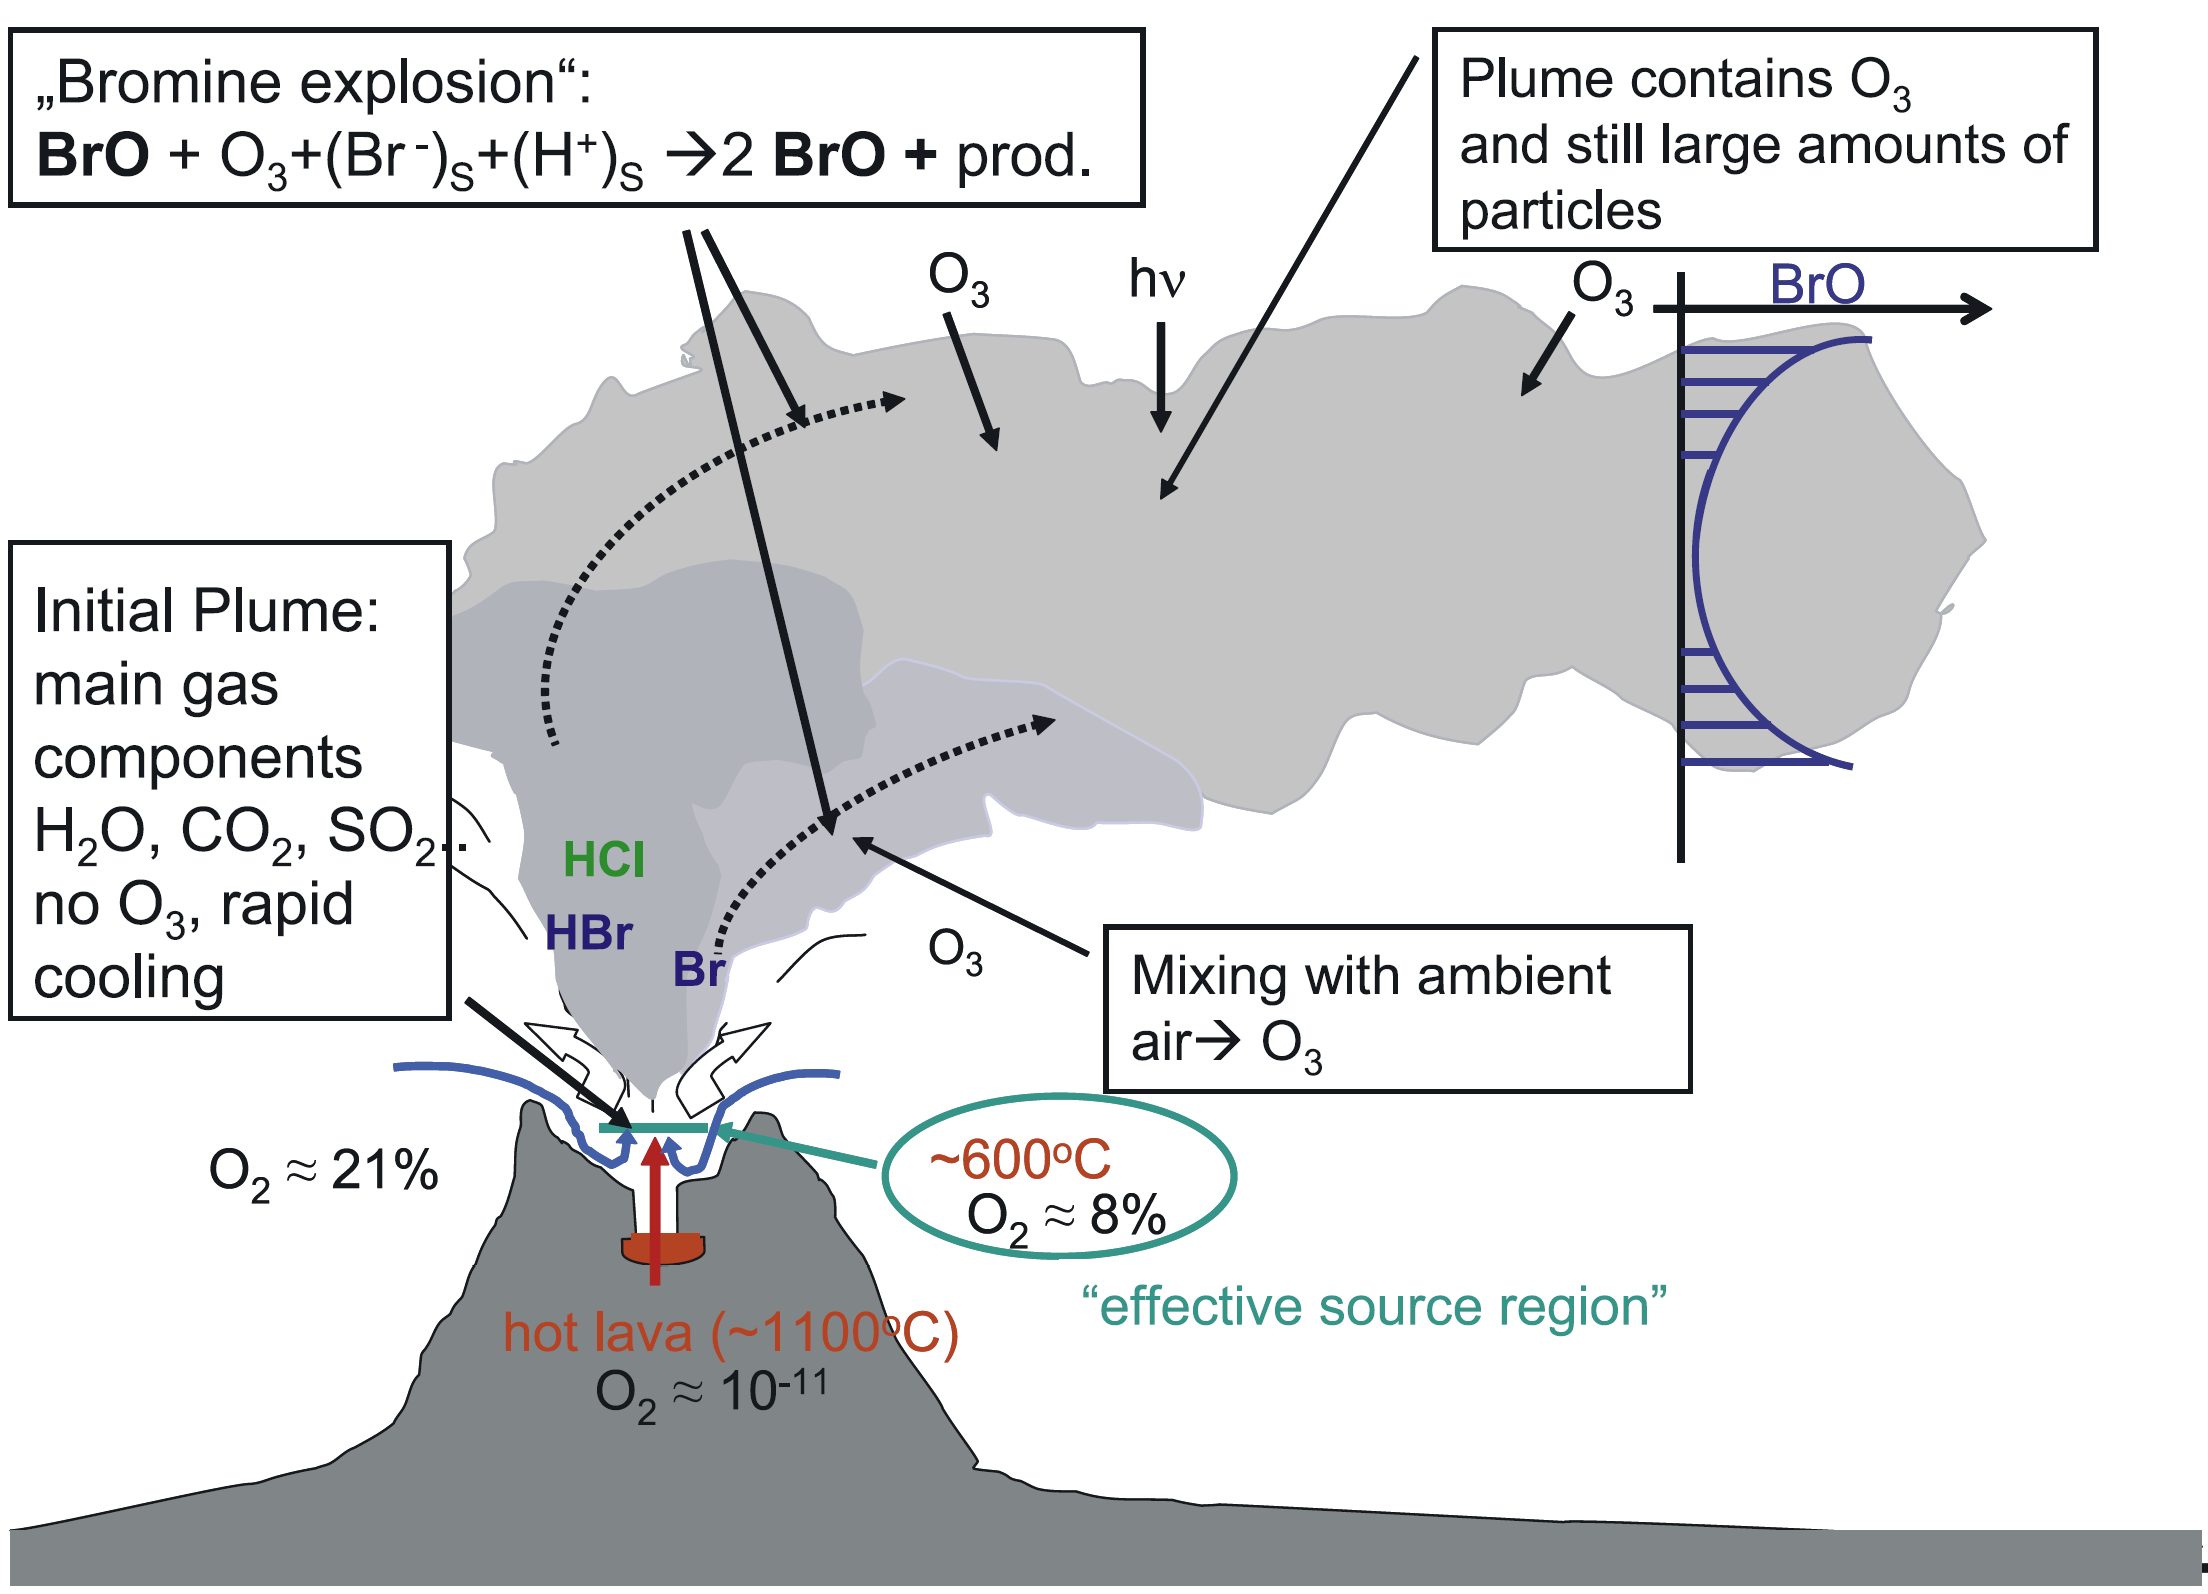
\includegraphics[width=0.7\linewidth]{Bilder/Simon/Bilder_Tung/BrO_Plume}
		\caption{schematic sketch of a Bromine Explosion.
			Release of \ce{HBr} at the volcanic vent. Mixing with ambient air in the effective source region leads to \ce{Br} formation. This resulting Bromine species react to \ce{BrO} with ozone from the plume. Adapted from \cite{bobrowski2007reactive}}
		\label{fig:broplume}
	\end{figure}
	\subsection{Volcanic gases and their impact on the climate}
	Volcanoes emit large amounts of gases into the atmosphere. In descending
	magnitude the most important gases are H2O, CO2, various sulphur species led
	by \ce{SO2} and H2S and halogen compounds (see Table 2.1). While water vapour is
	the most abundant gas in a volcanic plume, and responsible for the condensation
	of the plume that can be observed at many quietly degassing volcanoes from
	large distances, the total abundance is negligible when compared to evaporation
	from oceans. CO2 emissions are thought to have played an important role
	during the formation of Earth’s atmosphere. However, today CO2 emission
	from volcanoes are several orders of magnitude smaller than anthropogenic CO2
	emissions. While anthropogenic CO2 emissions were roughly 35 Gt (gigatons)
	in 2010, volcanic CO2 emission estimates ranged between 0.13 - 0.44 Gt per
	year, comparable to the CO2 emissions from countries as Pakistan (0.18Gt),
	Kazakhstan (0.25 Gt) or South Africa (0.44 Gt) (Gerlach, 2011, and references
	therein). However, on time scales of 105 a CO2 degassing has an important role
	in the Earth system, since it offsets CO2 burial in the sediments. \ce{SO2} is the
	third most abundant gas and can be measured by remote sensing in the UV. It
	is therefore often measured as a proxy for volcanic activity. The yearly global
	\ce{SO2} emissions by volcanoes range between 7.5 - 10.5TgSyr–1 (Halmer et al.,
	2002) and are therefore of the same magnitude as anthropogenic \ce{SO2} emissions
	(55TgSyr–1 for the year 2000 were given in IPCC, 2013).
	\ce{SO2} and \ce{BrO} are the two trace gases in volcanic plumes that are the main topic
	of this thesis. This chapter therefore gives a brief overview over the chemistry
	of \ce{SO2} and \ce{BrO} in the atmosphere after emission from the volcanic vent. The
	impacts of volcanic gas emissions on the environment and especially the influence
	of \ce{SO2} on the Earth’s climate will be discussed following Robock (2000). The
	part about \ce{SO2} summarizes parts of the review paper by Oppenheimer et al.
	(2011) and the chemistry of \ce{BrO} is based on the papers of Bobrowski et al. (2007)
	and von Glasow (2010). Both parts also contain ideas from von Glasow et al.
	(2009).
	Regardless of the path of \ce{SO2} scavenging,
	dry or wet deposition or oxidation
	to sulfuric acid, the molecule
	can influence the environment in several
	ways. A local effect, especially
	compared to the influences on the
	Earth’s climate, are direct influences
	of \ce{SO2} on humans (respiratory problems,
	asthma) and plants in the areas
	affected by volcanic gases. Acid rain
	caused by volcanic plumes can prevent
	the growth of plants. Darrall (1989)
	reviewed the influences of \ce{SO2} on photosynthesis,
	and found that long-term
	exposures with \ce{SO2} concentrations between
	100 - 250 ppb can inhibit photosynthesis
	of plants. Delmelle et al.
	(2002) measured \ce{SO2} concentrations
	around Masaya volcano, Nicaragua.
	The authors found concentrations of
	up to 230 ppb and an area downwind
	of the volcano with a decreased number
	of plant communities. Similar
	studies were done by Longo et al.
	(2005), who studied \ce{SO2} concentrations
	and fine aerosol downwind of Kilauea
	volcano on Hawaii. The authors
	found high \ce{SO2} concentrations of over
	61.9 ppb with atmospheric sampling in the Kau desert south of Kilauea crater.
	Despite these lower \ce{SO2} concentrations, plant growth is largely diminished in the
	Kau desert. Fig. 2.4 gives an impression of plants in the Kau desert. It should be
	noted, though, that while \ce{SO2} certainly has negative effects on plant life other
	species in the volcanic plume (e.g., HF) are most likely deposited within close
	proximity of \ce{SO2} on the ground as well.
	Sulphur influences on the Earth’s climate
	On a global scale, \ce{SO2} and especially its oxidation product sulphuric acid have
	a large impact on Earth’s climate. The total annual \ce{SO2} emissions are low
	compared with anthropogenic emissions. Halmer et al. (2002) estimated mean
	annual S emitted as \ce{SO2} by volcanoes between 1972 and 2000 to be in the range
	between 7.5 - 10.5TgSyr–1. The estimates for anthropogenic \ce{SO2} emissions for
	the year 2000 have a mean value of 55TgSyr–1 (IPCC, 2013). However, Graf et al.
	(1997) suggested that the impact of volcanic \ce{SO2} emissions is higher, since they
	are released into the free troposphere or into the stratosphere during eruptions,
	whereas most anthropogenic emissions are released into the planetary boundary
	layer. After emission into the atmosphere SO2, is oxidised to sulphuric acid. The
	lifetime of sulphuric acid in the troposphere is only about 1 week compared with
	up to one year in the stratosphere (IPCC, 2013).
	Sulphuric acid directly influences the climate by backscattering radiation
	from the sun and thus increasing the Earth’s albedo. Even more importantly
	it serves as additional cloud-condensation nuclei (CCN), which results in more
	and finer condensed particles and therefore in whiter, more-stable clouds and
	also an increased albedo of Earth (Twomey, 1974, and Fig. 2.5). This leads
	to more back-scattered radiation (see Fig. 2.5) and more diffusively scattered radiation. The net result of the back-scattered radiation is cooling of the Earth
	atmosphere, which is the dominating radiative effect of volcanic gases (Robock,
	2000). Additionally, aerosol particles can also act as surfaces for heterogeneous
	reaction cycles that destroy ozone, especially in the stratosphere, which leads to
	an increased solar flux to the Earth. Larger aerosol particles can backscatter IR
	radiation emitted from the Earth’s surface and the lower atmosphere and thus
	slightly reduce the net cooling effect in the lower troposphere. Absorption of
	direct UV and IR radiation from the sun as well as of radiation emitted by the
	Earth leads to net heating of the stratosphere. The 2013 IPCC report (IPCC,
	2013) states that the radiative forcing caused by volcanoes was -0.11 Wm-2
	between the years 2008 and 2011 (for comparison, the radiative forcing of CO2
	was given as 1.68Wm–2). Another, counter-intuitive effect is the winter warming
	in the Northern Hemisphere, which is caused by changes of the stratospheric and
	tropospheric circulation patterns due to strong temperature gradients between
	the Arctic and equatorial regions (Robock, 2000).
	\begin{figure}
		\centering
		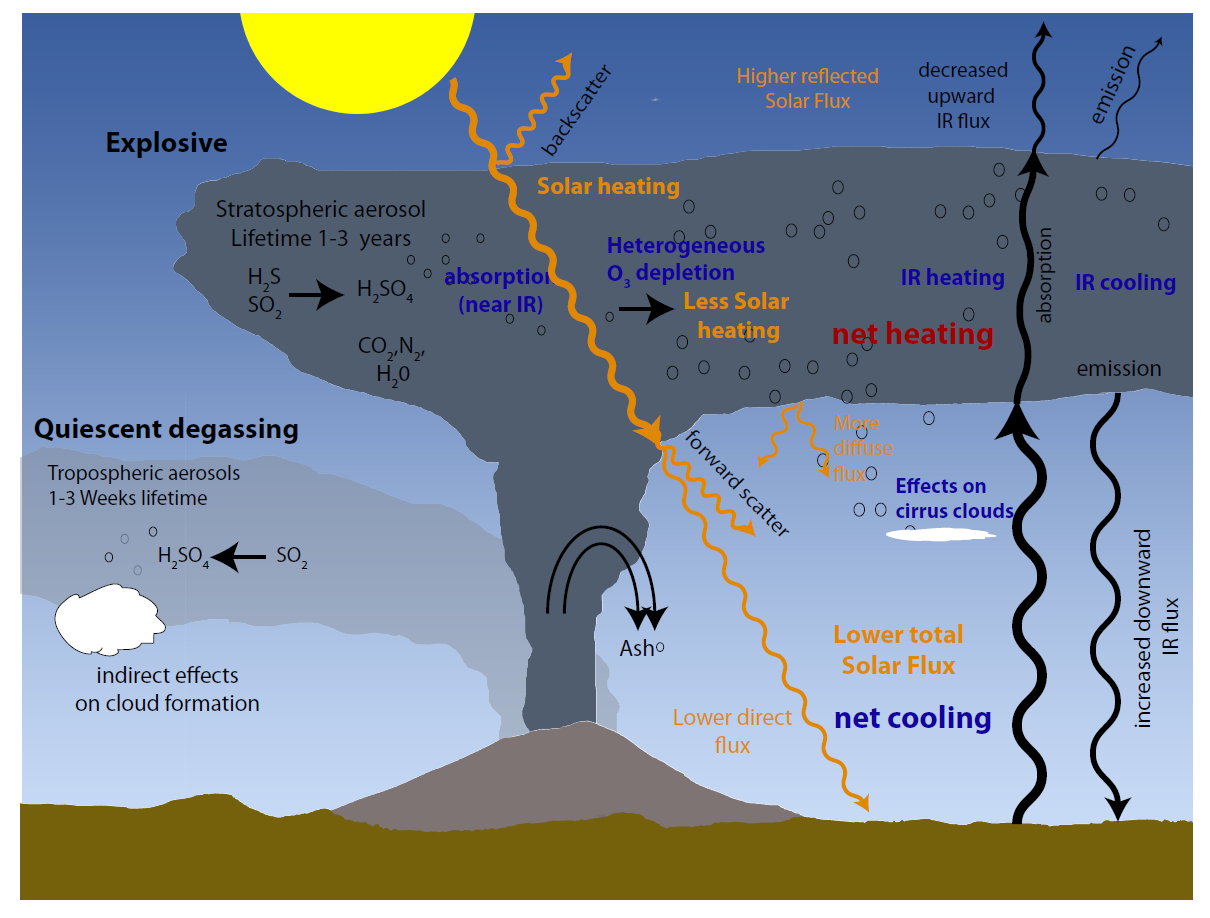
\includegraphics[width=0.7\linewidth]{Bilder/Simon/Bilder_Tung/Climate_Influence}
		\caption{Influence of volcanic eruptions and quiet degassing on earth climate. Redrawn on the basis of \cite{robock2000volcanic}}
		\label{fig:climateinfluence}
	\end{figure}
	\subsection{Volcanic plume chemistry}
	\begin{figure}
		\centering
		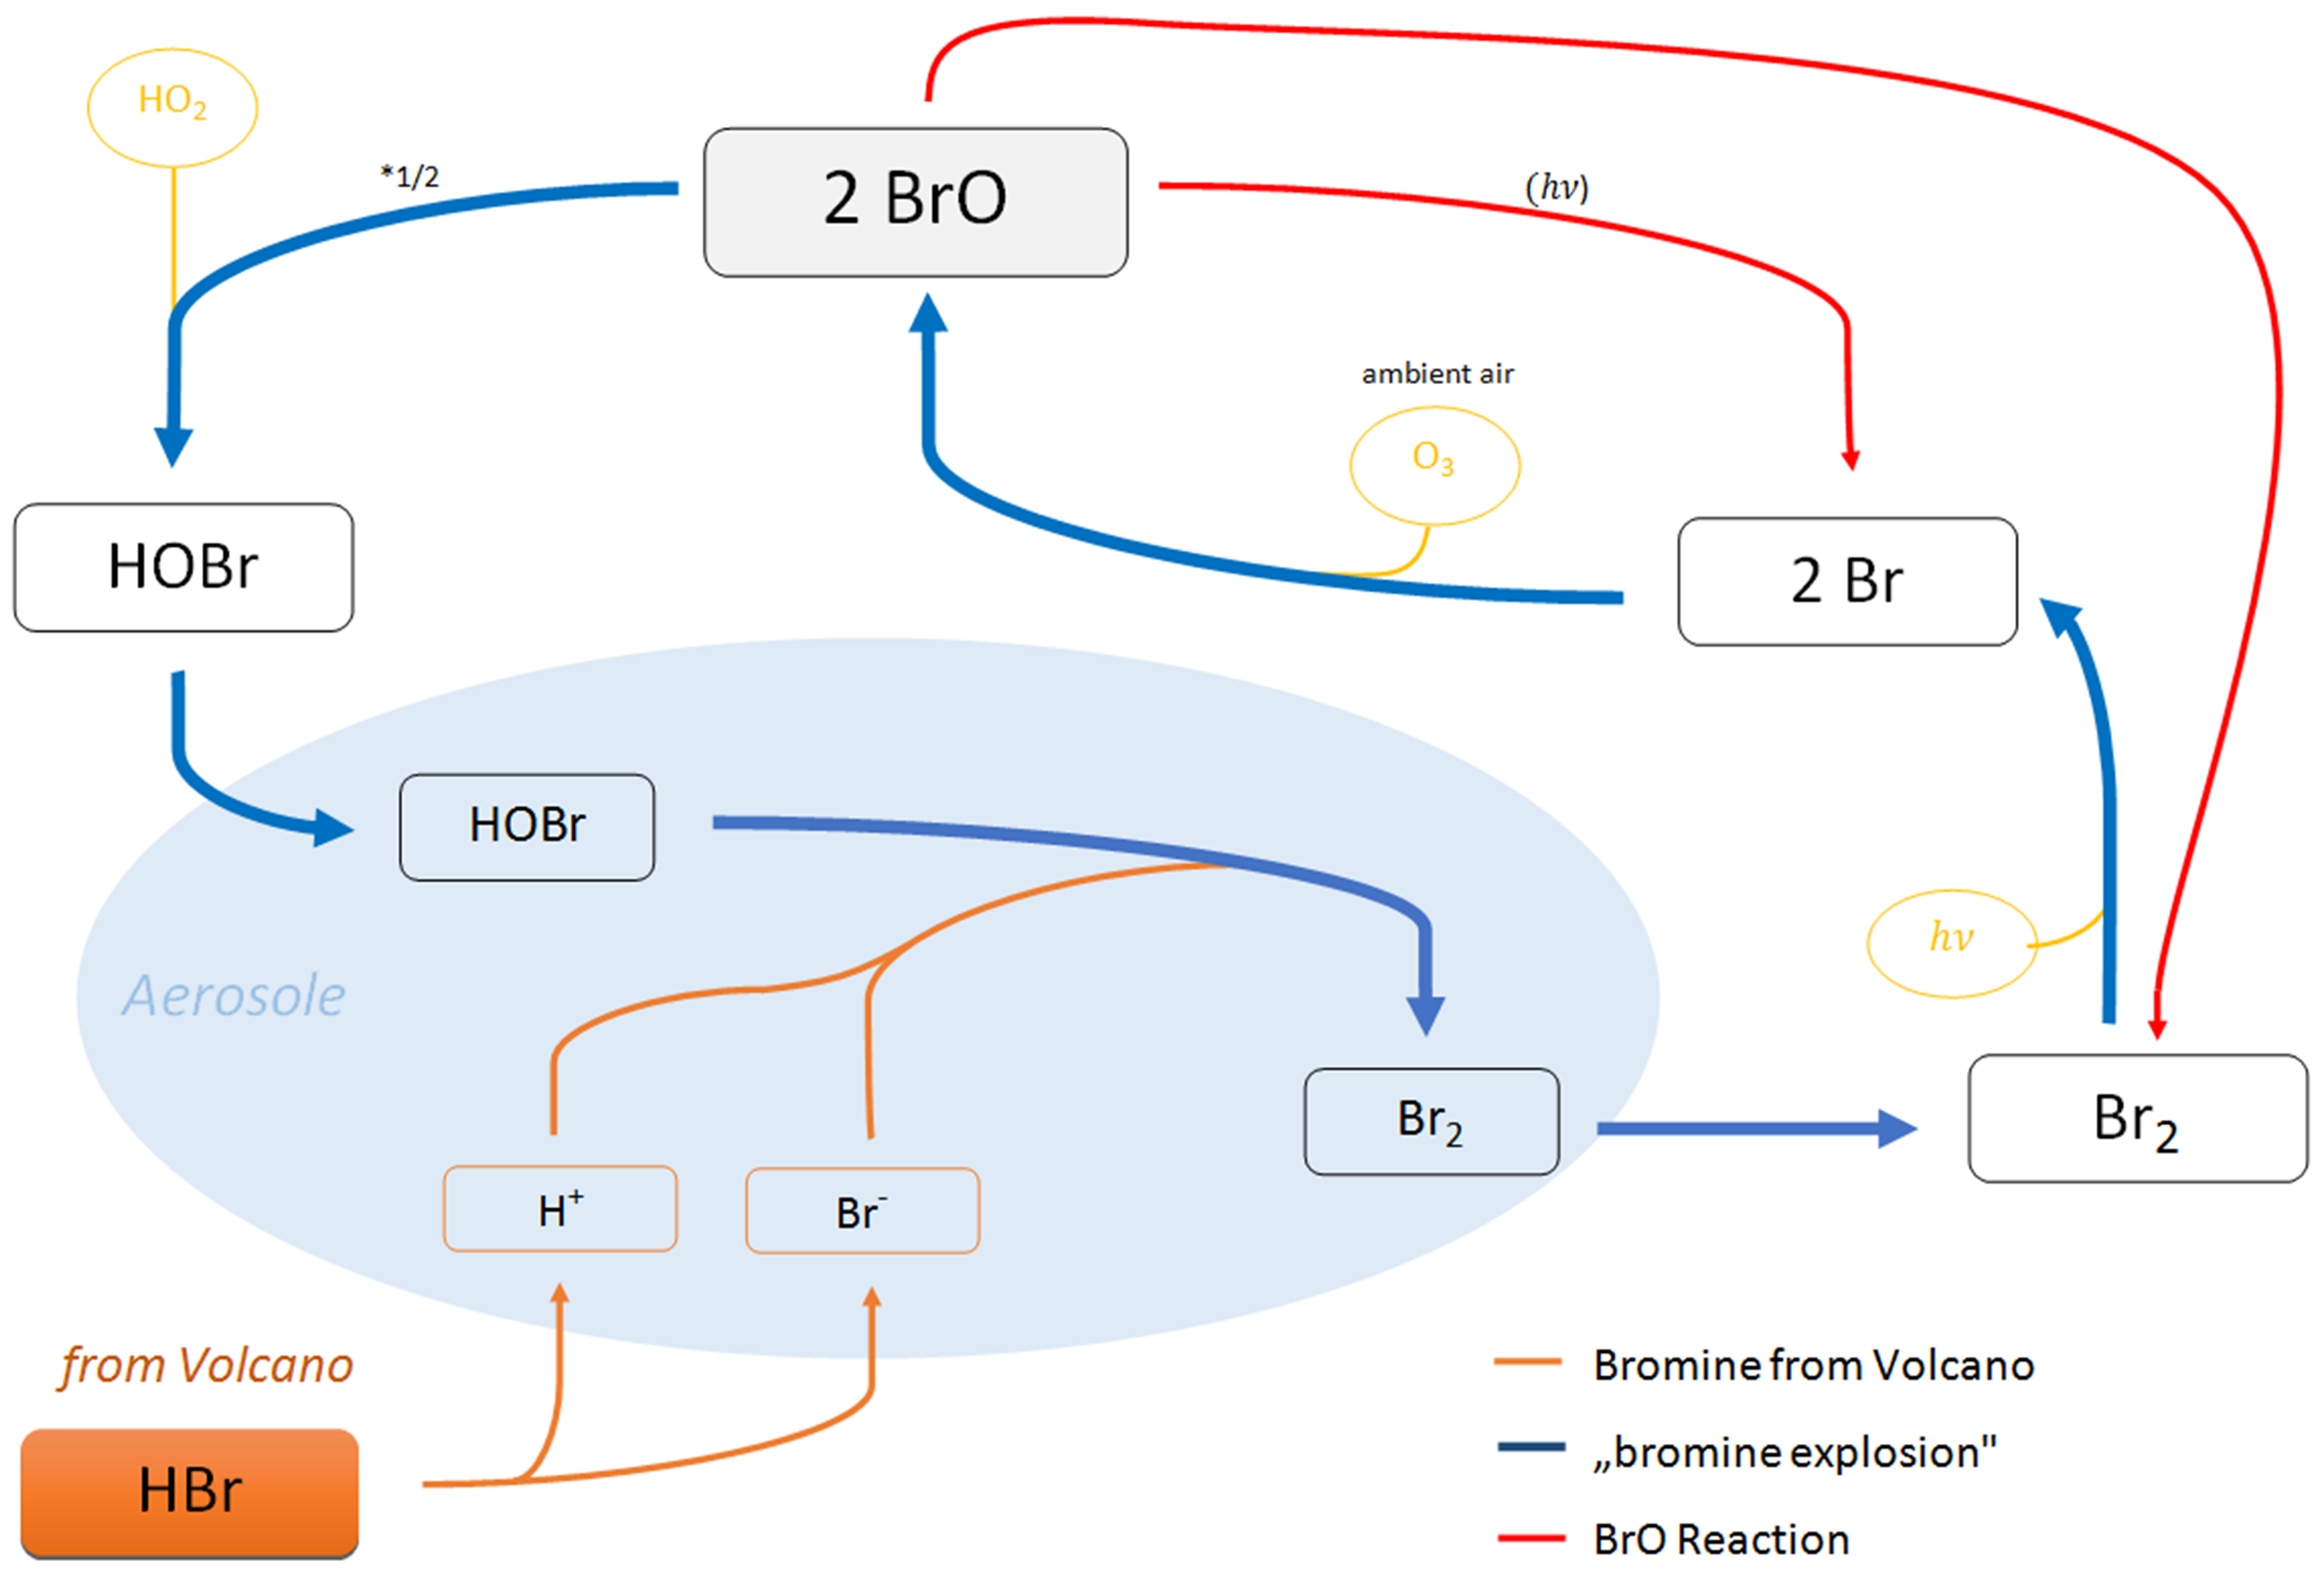
\includegraphics[width=0.7\linewidth]{Bilder/Simon/Bilder_Tung/BrO_Explosion}
		\caption{}
		\label{fig:broexplosion}
	\end{figure}}
	\subsection{Sulphur species}
	Sulphur species are the third most abundant gases in volcanic plumes, hereby contributes SO2 with about 25\% and \ce{H2S} with 1 to 10\%. Only \ce{H2O} and \ce{CO2} have a larger share on the volcanic gases in the plume.
	
	
	
	
	
	
	
	
	
	
	
	
	
	
	
	
	
	
	
	
	
	
	
	\textcolor{red}{
	2.3.1 Sulphur species
	Sulphur species, mainly \ce{SO2} and H2S are the third most abundant species in
	volcanic plumes after H2O and CO2. \ce{SO2} contributes up to 25% of the total
	volume of the volcanic plume and H2S ranges between 1 - 10% (see Table 2.1).
	As opposed to the two most dominant species, \ce{SO2} does not have considerable
	background levels in the atmosphere. The \ce{SO2} concentration in the atmosphere
	is usually below 1 ppb while the concentration in a volcanic plume can easily
	achieve levels of 1 ppm (Oppenheimer, 2003a). The low background values
	together with the stability and the relatively strong UV absorption make SO2
	an easily accessible tracer for volcanic gas emissions (see next Section 2.4).
	After their release from the reducing conditions in the volcanic vent the gases
	enter the atmosphere, which is an oxidising environment. H2S is slowly oxidized
	to \ce{SO2} when released into the atmosphere. The first step is the reaction of SH
%	with OH:2
%	H2S + OH −−−−−−−!
%	k=4.7×10−12 H2O + SH (C 2.1)
	The SH radical then undergoes a series of reactions in the atmosphere that
	lead to the formation of \ce{SO2} (Seinfeld and Pandis, 2006). Theoretically H2S
	can react with the halogen radicals Cl and Br to form SH, which results in H2S
	lifetimes of only a few seconds (Aiuppa et al., 2007). However, Aiuppa et al.
	(2007) could not reproduce these low H2S lifetimes in measurements that showed
	a constant SO2/H2S ratio at distances up to several kilometres from the vent.
	\ce{SO2} is removed from the atmosphere by wet and dry deposition or oxidized to
	sulphuric acid. In the gaseous phase the reaction with OH to sulphuric acid is
	rather slow:
%	SO2 + OH M
%	−−−−−−−!
%	k=1.3×10−12 HSO3 (C 2.2)
%	HSO3 + O2 −−−−−−−!
%	k=4.3×10−13 HO2 + SO3 (C 2.3)
%	SO3 + H2O M
%	−−−−−−−−!
%	k=5.7×104 s−1 H2SO4 (C 2.4)
	The rate constant k in Eq. C2.4 is given for 50% humidity in Atkinson
	et al. (2004). Möller (1980) calculated an \ce{SO2} loss rate of k = 1.2 10-6 s-1 for
	homogeneous reactions in the gas phase, or converted to hours a loss of 0.43%
	\ce{SO2} per hour. In heterogeneous reactions, such as reactions of \ce{SO2} on particles
	or in the liquid phase of particles, the oxidation process is much faster. Möller
	(1980) gave loss rates of k = 0.1- 1 10-5 s-1 for reactions of \ce{SO2} on aerosol
	particles and k = 5 10-5 s-1 for liquid phase oxidation. The equations for the reaction of \ce{SO2} in the liquid phase are (Möller, 1980):
%	SO2,g + H2Oaq −)−−*− (SO2 · H2O)aq (C2.5)
%	(SO2 · H2O)aq + H2O −−* )−− HSO−3,aq + H3O+
%	aq (C 2.6)
%	HSO−3 + H2O −)−−*− SO2−
%	3 + H3O+ (C 2.7)
%	HSO–3 and SO2–
	3 can be further oxidized to sulphuric acid or sulphate, e.g. by a
	reaction with OH (Platt and Stutz, 2008). The oxidation of SO2 can also take
	place on aerosol particles by reactions with O3, H2O2, HOCl, HOBr or oxygen if
	catalysts (iron, manganes) are available (von Glasow et al., 2009).
	Considering these different pathways and regarding the importance of \ce{SO2} as
	a tracer for volcanic activity and for the comparison of \ce{SO2} with other trace
	gases, it is worthwhile to compare measured \ce{SO2} loss rates with the values given
	above. There are only a few reports of high \ce{SO2} loss rates. Jaeschke et al.
%	(1982) and Oppenheimer et al. (1998) reported loss rates between 110−3 s−1
	and 7  10-4 s-1, which would lead to an e-folding time between only 16 and
	23 minutes. However, older data listed in Oppenheimer et al. (1998) showed
%	loss rates between 5  10−5 s−1 and 210−7 s−1, therefore leading to e-folding
	times between 5 hours and several weeks. McGonigle et al. (2004) studied the
	depletion rate of \ce{SO2} using the DOAS technique at Masaya volcano, Nicaragua.
	The authors found that there are negligible variations of up to 500 s - 2000 s
	after release from the volcano. Furthermore, the authors argue that Jaeschke
	et al. (1982) had problems with using CO2 as a tracer to compare the SO2
	concentration. Meanwhile Oppenheimer et al. (1998) based the calculated loss
	rates on only a few traverse measurements, thus being influenced by variations
	in the total emission rate from the volcano as well as errors from wind speed and
	direction. Oppenheimer et al. (1998) measured ash plumes during the wet season
	at Soufriere Hills, Montserrat. Repeated measurements at the same volcano with
	more traverses during the dry season and ash-free volcanic plumes, found an one
	order of magnitude slower \ce{SO2} loss rate (Rodríguez et al., 2008). Recent studies
	from satellites by Beirle et al. (2013) investigated the \ce{SO2} loss rates at Kilauea,
	Hawaii. The authors found mean monthly \ce{SO2} life times between 16 and 57 h,
	with the longer lifetimes in summer, when the cloud coverage is lower. While
	satellites are not able to assess potential \ce{SO2} loss close to the volcanic vent due
	to restrictions of their spatial and time resolution, this study still shows slow
	\ce{SO2} loss rates with robust observations over a long time-scale.
	In this work it is assumed that \ce{SO2} is stable during the time frame that usually
	occurs during ground-based remote sensing measurements (a few up to several
	tens of minutes during this thesis).
	\subsection{Bromine oxide}
		2.3.2 Bromine oxide
	Bromine oxide (BrO) was detected for the first time at Soufriere Hills volcano
	(Montserrat) by Bobrowski et al. (2003). Since then, \ce{BrO} has been detected
	at many volcanoes by ground-based measurements (e.g., Bobrowski and Platt,
	2007; Bobrowski et al., 2007; Oppenheimer et al., 2006; Vogel, 2011) or from
	airborne platforms (Heue et al., 2011; Kelly et al., 2013). Theys et al. (2009)
	were able to detect \ce{BrO} from satellite after the Kasatochi eruption in 2008, and
	Hörmann et al. (2013) were able to find \ce{BrO} in volcanic plumes from 11 erupting
	volcanoes with data from the GOME-2 instrument.
	However, it is actually mainly HBr, not BrO, that is emitted from volcanoes.
	\ce{BrO} is formed after the volcanic gas mixes with ozone-rich ambient air. Gerlach
	(2004) and Martin et al. (2006) used thermodynamical equilibrium calculations
	to assess the source of bromine and found that there is not enough Br or BrO
	in hot magmatic gases to explain the \ce{BrO} concentration measured, e.g. at
	Soufriere Hills by Bobrowski and Platt (2007). Instead, the volcanic gases mix
	with atmospheric air at high temperatures, in the so-called effective source region
	(Bobrowski et al., 2007), see Figure 2.6. This can be compared to a chimney,
	where hot air released from the volcano pulls in atmospheric air through the
	permeable edifice (Gerlach, 2004). The mixing process at high temperatures
 changes the gas composition and leads to an increase in bromine
	species other than HBr such as Br, Br2 and \ce{BrO} (Martin et al., 2006; von Glasow,
	2010). Further mixing with atmospheric air leads to cooling down to ambient
	temperatures where the so-called Bromine Explosion starts. The term Bromine
	Explosion originates from \ce{BrO} observations in polar regions, where a similar
	non-linear increase in \ce{BrO} concentration has been observed (Hönninger and
	Platt, 2002; Lehrer et al., 1997; Wennberg, 1999).
	The Bromine Explosion mechanism can be summarized as:
%	HBrgas −−! Br−
%	aq + H+
%	aq (C 2.8)
%	HOBr(gas) −−! HOBr(aq) (C 2.9)
%	HOBr(aq) + Br−
%	(aq) + H+
%	(aq) −−! Br2(aq) + H2O (C 2.10)
%	Br2,aq −−! Br2,gas (C 2.11)
%	Br2 + h −−! 2 Br (C 2.12)
%	Br + O3 −−! \ce{BrO} + O2 (C 2.13)
%	\ce{BrO} + HO2 −−! HOBr + O2 (C 2.14)
%	\ce{BrO} + \ce{BrO} −−! 2 Br + O2 (C 2.15)
%	\ce{BrO} + \ce{BrO} −−! Br2 + O2 (C 2.16)
	C2.8 and C2.9 describe the uptake of HBr and HOBr on the surface of an
	aerosol particle and subsequent transformation into the liquid phase. At low pH
	< 6.5 (Fickert et al., 1999) or at cold temperatures H+, Br– and HOBr react to
	form Br2 (C 2.10) that is then released back into the gas phase (C 2.11). Br2
	reacts to Br via photolysis if sunlight is available (C 2.12). The necessity of solar
	radiation for the Bromine Explosion in volcanic plumes was verified by Kern et al.
	(2009), who could measure elevated \ce{BrO} during daytime, but not at night at
	Masaya volcano, Nicaragua. In the next step Br that was formed from Br2 and
	O3 reacts to \ce{BrO} (C 2.13). The role of O3 in Eq.C2.13 was shown by Bobrowski
	et al. (2007) and Louban et al. (2009) who measured higher \ce{BrO}/\ce{SO2} ratios at
	the edges of the volcanic plume rather than in the middle of the plume, where
	less ambient (ozone-rich) air is available. Kelly et al. (2013) was able to measure
	the evolution of ozone depletion in volcanic plumes from an airborne platform.
	\ce{BrO} can react with HO2 to form HOBr again leading back from C2.15 to C2.9.
	The result of this reaction cycle is the formation of \ce{BrO} and the destruction of
	O3. \ce{BrO} can also react with another \ce{BrO} molecule to form Br2 or Br (C. 2.15
	and 2.16), which in turn would react again to BrO. The Bromine Explosion
	reaction cycle is schematically shown in Figure 2.7.
	Considering the multitude of chemical reactions that take part in the formation
	of \ce{BrO} and because \ce{BrO} is a secondary volcanic gas, there is some discussion as to
	whether \ce{BrO}/\ce{SO2} ratio can be a useful indicator of volcano activity. If \ce{BrO}/\ce{SO2} ratios are used as an indicator of volcanic activity, influences from the formation
	of \ce{BrO} in the atmosphere have to be ruled out or characterized carefully. \ce{SO2} can
	be regarded as stable during times that are typically observed in ground-based
	remote sensing observations (see above). Perspectives on the time scales of BrO
	formation have changed over the last couple of years. Bobrowski et al. (2007)
	and Roberts et al. (2009) estimated an increase in the \ce{BrO}/\ce{SO2} ratio up to
	several tens of minutes after release from the vent. Newer publications and an
	improving dataset led Bobrowski and Giuffrida (2012) to the conclusion that the
	\ce{BrO}/\ce{SO2} ratio increases in the first minutes after release from the volcano, and
	then stays constant for some time (see Figure 2.8). Vogel (2011) and Gliß (2013)
	were able to measure the evolution of the \ce{BrO}/\ce{SO2} ratio in the young plume of
	Pacaya volcano and Etna volcano respectively using horizontal DOAS scanning
	measurements and found a strong increase within the first five minutes after
	release. Vogel (2011) also measured the \ce{BrO}/\ce{SO2} ratios in ageing plumes at Mt.
	Etna and found a constant ratio for plume ages of up to two hours. It has not
	been sufficiently examined if the \ce{BrO}/\ce{SO2} ratio depends on the ratio of Br/S
	exsolved from the magma. Nevertheless, it is import to rule out influences of
	atmospheric chemistry in order to find a meaningful interpretation of \ce{BrO}/SO2
	ratios. The influence of the time following the mixing of volcanic gas with the
	ambient atmosphere will be discussed in Chapter 5.
	\subsection{Using volcanic gases to study volcanic activity}
	\begin{figure}
		\centering
		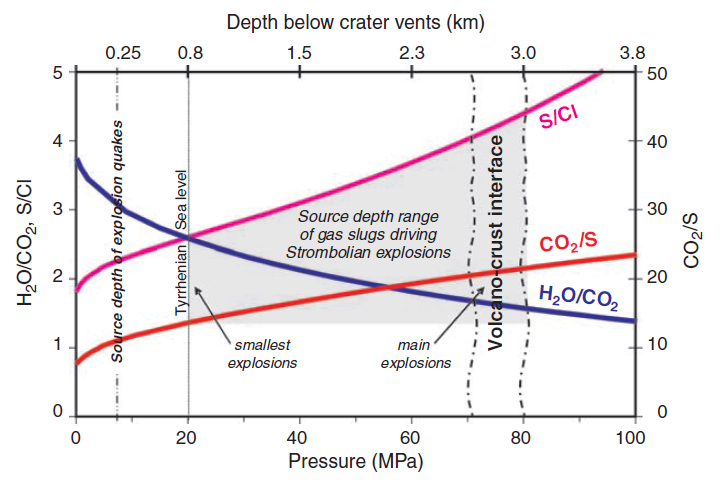
\includegraphics[width=0.7\linewidth]{Zwischenbericht2018/Bilder/so2_bro}
		\caption{Dependency of the ratios of different volcanic trace gases on depth. Data originate from Stromboli volcano. From \cite{lubcke2014optical} reproduced from Burton et al. (2007)}
		\label{fig:so2bro}
	\end{figure}	
	2.4 Using volcanic gases to study volcanic activity
	There are many factors influencing the degassing of volatiles and the composition
	of gases after and during the release from the volcanic vent. Furthermore the
	plume composition changes when it reacts with the oxidizing atmosphere. Therefore
	interpreting volcanic degassing data is complex. For example, Oppenheimer
	et al. (2011) reported in their review paper on \ce{SO2} degassing, that decreasing
	\ce{SO2} fluxes have been ascribed to:
	• depletion of volatiles in a magma body
	• decreased permeability of the magma in the conduit
	The first process can be regarded as an indicator of decreasing volcanic activity.
	The second process can be caused by, for example, the formation of a plug when
	degassed magma starts crystallization. The plug leads to a build up of gas
	pressure and ultimately might lead to an eruption (Clarke, 2013). Therefore the
	observation of decreasing \ce{SO2} emission rates can indicate an increase as well as
	a decrease of volcanic activity.
	Despite these complications, measurements of volcanic gases can be an important
	additional tool for the forecasting of volcanic activity to accompany
	the classic monitoring techniques like seismicity or deformation measurements.
	The remote sensing of volcanic gases started with the correlation spectrometer
	COSPEC (Moffat and Millan, 1971; Stoiber et al., 1983) in the 1970 s. COSPEC 
	measurements together with fumarolic sampling helped, for instance, predict the
	eruptions of Mount St. Helens, USA, in August 1980 and June 1981 (Casadevall
	et al., 1983) or Pinatubo, Philippines, in 1991. The remote sensing of volcanic
	\ce{SO2} experienced further spreading world-wide with the availability of miniature
	spectrometers (Galle et al., 2003) that measure the \ce{SO2} column density by
	using Differential Optical Absorption Spectroscopy (DOAS, Platt and Stutz,
	2008). Besides being smaller and cheaper, these miniature spectrometers using
	the DOAS technique have additional advantages for fieldwork in rugged
	environments, as they are lighter and consume less power. Additionally the
	availability of more spectral information allows for the correction of radiative
	transfer problems (Kern, 2009, and also Chapter 3) and to retrieve other trace
	gases (e.g. O3, NO2 or BrO). An important step towards continuous monitoring
	of volcanic \ce{SO2} emission rates was made with the Network for Observation
	of Volcanic and Atmospheric Change (NOVAC, Galle et al., 2010). During
	this EU-funded project scanning DOAS instruments were installed at several
	volcanoes world-wide. The spectroscopic data for the \ce{BrO}/\ce{SO2} ratios evaluated
	within this thesis were recorded by the NOVAC network, which will be discussed
	in more detail in Chapter 5. Besides the monitoring instruments and the network
	itself, the detection of abnormally high \ce{SO2} emission rates at Santa Ana volcano
	(El Salvador) before the eruption in 2005 was the first big success of the project
	(Olmos et al., 2007). These measurements helped to plan the evacuation of
	thousands of people living in the vicinity of Santa Ana volcano. Scanning DOAS
	instruments need approximately 5 – 15 minutes for one scan across the complete
	sky. These techniques are therefore rather suited to measure long-term variations
	in the \ce{SO2} emission rates.
	A lot of additional information can be gained when using instruments that
	allow emission rate measurements with a higher time resolution. Boichu et al.
	(2010) used two spectrometers with an optical system that led to a wide fieldof-
	view covering the complete volcanic vent at Mount Erebus, Antartica. This
	set-up allowed \ce{SO2} emission rate measurements with a time resolution of the
	order of 1 Hz. Frequency analysis of the data revealed patterns with periods
	between 11 and 24 minutes that allowed discussion of different models for the
	degassing at Mt. Erebus. The \ce{SO2} camera, which is also used in large parts of
	this thesis, makes \ce{SO2} emission rate measurements with a similar time resolution
	possible. Holland et al. (2011) used \ce{SO2} camera measurements at Santiaguito,
	Guatemala to identify shear-fracturing as the main process leading to cyclic
	patterns of explosive eruptions rather than building of a viscous plug. Tamburello
	et al. (2013) applied \ce{SO2} cameras at Etna, Italy, using a similar approach as
	Boichu et al. (2010), and suggested that periodic signals with periods between
	40 – 250 s and 500 – 1200 s are caused by bursting of rising gas bubbles. First
	steps in the direction of the analysis of high time resolution \ce{SO2} camera data
	are presented in Chapter 4 of this thesis.
	In addition to the \ce{SO2} emission rate, the ratio between different trace gases can
	be indicative of volcanic activity as well. The solubility of volatiles depends, e.g.
	on depth and chemical composition of the magma (see Chapter 2.1), therefore
	the composition of volcanic gases has been studied in depth. A good introduction
	to gas compositions and their interpretation can be found in Giggenbach (1996).
	A more recent review article about halogens in volcanic system was published by
	Aiuppa et al. (2009). Initial studies (e.g. Noguchi and Kamiya, 1963) investigated
	the Cl/S ratio by direct sampling. The authors found a decrease of the Cl/S
	ratio before an eruptive period (Noguchi and Kamiya, 1963; Stoiber and Rose,
	1970). Later Pennisi and Le Cloarec (1998) found that Cl and F degas in a
	similar manner, while the Cl/S ratio varied between non-eruptive and eruptive
	periods. The authors argue that chlorine is exsolved from the magma at deeper
	levels (Cl/S > 1) while at shallower levels sulphur degassing dominates (Cl/S
%	 0.1). Burton et al. (2007) measured volcanic gas composition (H2O, CO2,
	CO, \ce{SO2} and HCl) by remote sensing using an open-path Fourier transform
	infrared spectrometer (OP-FTIR) at Stromboli, Italy. The authors found that
	the ratio of CO2/\ce{SO2} and SO2/HCl were 3-5 times higher during explosions than
	during quiescent degassing. These observations paired with higher equilibrium
	temperatures lead the authors to the conclusion that the explosions are driven by
	gas slugs that originate from a deeper level than gas observed during quiescent
	periods. The authors then used melt inclusion data and a chemical model
	simulating degassing of magma to interpret the data. The S/Cl and H2O/CO2
	ratios show that bigger explosions originate from a depth of approximately
	2.7 – 3km while smaller eruptions originate from depths as shallow as 0.8 km
	below the crater at sea level.
	The \ce{BrO}/\ce{SO2} ratio has been measured using DOAS remote sensing measurements
	by several authors (e.g., Bobrowski and Platt, 2007; Bobrowski et al.,
	2003, 2007; Hörmann et al., 2013; Kelly et al., 2013; Oppenheimer et al., 2006;
	Theys et al., 2009; Vogel, 2011). However, despite naming the possibility to
	use \ce{BrO}/\ce{SO2} ratios as an additional tracer for volcanic activity, most of these
	studies focused on the formation of \ce{BrO} in the atmosphere. First long-time
	measurements at Etna, Italy, were published by Bobrowski and Giuffrida (2012).
	The authors measured the \ce{BrO}/\ce{SO2} ratio covering the years 2005 - 2009 and
	found higher ratios during non-eruptive periods. During four eruptive periods
	\ce{BrO}/\ce{SO2} ratios were higher three months before the eruption compared to the
	ratios observed one month before the eruption. Studies on the seasonal variability
	and the influence of humidity did not reveal obvious correlations. The authors
	suggested a model in which bromine is released earlier than sulphur during the
	magma’s ascent to explain the observed behaviour.}
	\subsection*{Tungurahua}
	Tungurahua is a subduction zone volcano located in the Ecuadorian Andes (Lat: 01$^{\circ}$,28$^{'}$S; Long:78$^{\circ}$,27$^{'}$W). 2014 Tungurahua was one of the most active volcanoes in southern America, since then the activity was decreasing. Tungurahua is 5023m high and is one of the defining volcanoes of the eastern volcanic rows in Ecuador. \cite{hall1999tungurahua}
		
	\subsection*{Nevado Del Ruiz}
	Nevado Del Ruiz is also a subduction zone volcano. 	Nevado Del Ruiz  is located in the Central Cordillera of Colombia, 140 km west of Bogota.
	(Lat: 04$^{\circ}$,53$^{'}$S; Long:75$^{\circ}$,19$^{'}$W) 
	The hight of Nevado Del Ruiz is 5389 m.
	 
	\chapter{Remote sensing of volcanic gases}
	In this thesis we are interested in the volcanic trace gases \ce{SO2} and BrO, both measured with the Differential Optical Absorption Spectroscopy (DOAS) a remote sensing technique proposed by \cite{platt2008differential}\\
	

	\section*{Beer-Lambert Law}
	The Lambert-Beer law describes the attenuation of light when traveling through a material.\\
	This section will give an overview about the reasons for decreasing light intensity when going through a medium.\\
	Atoms and Molecules exists in several energy states, depending on the different electron configuration. Moreover Molecules have additionally rotation and vibration states, also enclose to the energy states. If a photon matches the energy gap between two possible energy states, this includes, that the lower energy state is occupied and the selection rules are fulfilled  the molecule could absorb the photon, remaining in a higher energy state.\\
	The additional photon energy could be loosed by collision with another molecule or by emission. But since the direction of the emitted photon is mostly not the same direction of the absorbed photon the intensity I$_{0}$ of the light before passing the medium is higher than the intensity I after traveling the distance L through the medium.\\
	This can be described as:\\ 
	\begin{equation}
	I\left(L,\lambda\right) = I_{0}\left(\lambda\right)\cdot expt\left(-\int^{L}_{0}\sigma\left(\lambda,p,T\right)\cdot c\left(l\right)dl\right)
	\end{equation}
	where $c\left(l\right)$ is the location-dependent concentration of the trace gas of interest. $\sigma\left(\lambda,p,T\right)$ is the absorption cross section, $\sigma\left(\lambda,p,T\right)$ is unique for each molecule and depends on pressure p and on the temperature T.\\
	%
	An important quantity used in many optical remote sensing techniques is the optical density $\tau$. The optical density is a measure for the weakening of radiation when going through a material. $\tau$ can be calculated using the lambert beer law:
	\begin{equation}
	\tau = -ln\left(\frac{I\left(\lambda\right)}{I_{0}\left(\lambda\right)}\right) = \sigma\cdot S
	\end{equation}
	Hereby is $S$ the column density. The column density is the concentration of the trace when integrating along the light path, the dimension of $S$ is therefore the number of molecules divided by an area: $\frac{molec}{cm^2}$.
	\begin{equation}
	S = \int_{0}^{L}c\left(l\right)dl
	\end{equation}
	%
	When measuring at a volcano, that means measuring in the atmosphere the situations gets more complex, since we need to deal with several absorbers and scattering processes have to be taken into account. One possibility is to treat scattering effects as pseudo absorbers with the respective extinction coefficients for Rayleigh ($\epsilon_R$) and  Mie ($\epsilon_M$) scattering
	\begin{equation}
	I\left(L,\lambda\right) = I_{0}\left(\lambda\right)\cdot expt\left(-\int^{L}_{0}\sum_{j}\sigma_{j}\left(\lambda,p,T\right)\cdot
	c_{j}\left(l\right)+\epsilon_R\left(\lambda,l\right)+\epsilon_{M}\left(\lambda,l\right)dl\right)
	\label{eq:lbe}
	\end{equation}
	The first term of \cref{eq:lbe} in the exponential function, multiple absorbers $j$ are considered, the corresponding concentration depends on the position l of the light path.
	The last two terms in describe the extinction due to Rayleigh and Mie scattering in the atmosphere.\\
	Inelastic scattering (for example the Ring effect) and effects due to turbulences in the atmosphere are neglected here.

	\section{Differential Optical Absorption Spectroscopy(DOAS)\label{DOAS}}
		\begin{figure}
			\centering
			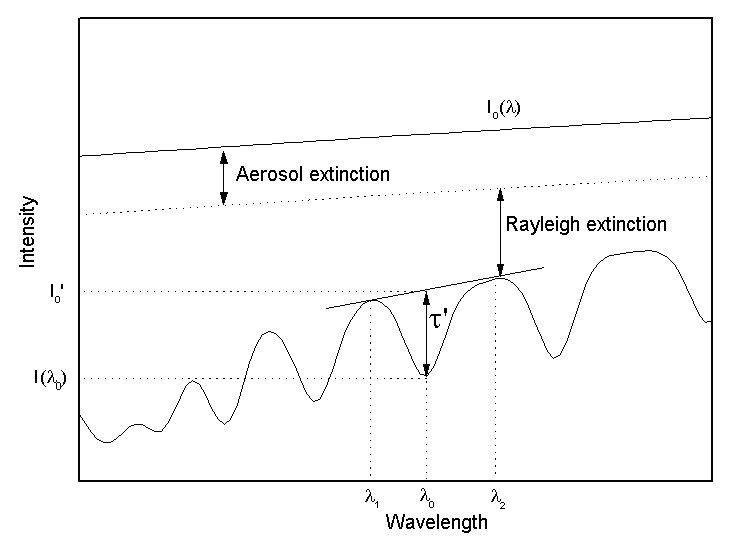
\includegraphics[width=0.7\linewidth]{Bilder/Simon/Bilder_Tung/DOAS_Intensity}
			\caption{Basic idea of the DOAS principle: Light attenuate due to broad band and narrow band effects. The broad band extinction is caused by aerosols and Raylight scattering $\left(I_0\rightarrow I^{'}\right)$. The measured intensity $I$ is formed by narrow band effects due to differential absorption structures by trace gases with the optical density $\tau^{'}$. Adapted from \cite{kern2009spectroscopic}}
			\label{fig:doasintensity}
		\end{figure}
		
	It is impossible to distinguish between various broad-band effects, like scattering in the atmosphere or instrument effects which influence the measured spectra \cite{lubcke2014optical}. Therefore \cref{eq:lbe} cannot be applied to real measurements.\\
	Differential Optical Absorption Spectroscopy (DOAS) was invented in the late 1970s by \cite{perner1979detection}. This section will give an overview about the DOAS technique. More detailed information ca be found in the work of \cite{platt2008differential}\\
	\newline
	Differential Optical Absorption Spectroscopy uses the fact, that absorption can be divided into broad-band parts and narrow-band parts. Broad band parts are effects that only changes weakly with the wavelength,  i.e. scattering and instruments effects have a broad-band structure. 
	The narrow band part includes effects that strongly depends on the wavelength.
	Within the DOAS-Method only narrow-band absorption features of molecules are used to obtain their column densities.
	The absorption cross section of trace gases $j$ have broad-band ($\sigma_b\left(\lambda \right)$) and narrow band ($\sigma{'}\left(\lambda \right)$) features, only the narrow-band structures are used in DOAS.
	\begin{equation}
	\sigma\left(\lambda \right) = \sigma_b\left(\lambda \right) + \sigma{'}\left(\lambda \right)
	\end{equation}
	%
	With this considerations the Lambert-Beer law \cref{eq:lbe} can be rewritten
	dividing the exponential part into a narrow-band part and a broad-band part:

	\begin{align}
	I\left(\lambda,L\right) = &\overbrace{I_{0}\left(\lambda\right)\cdot exp\left(-\int^{L}_{0}\sum_{j}\sigma_{b,j}\left(\lambda,p,T\right)\cdot c_{j}\left(l\right)+\epsilon_R\left(\lambda,l\right)+\epsilon_{M}\left(\lambda,l\right)dl\right)}^{=I^{'}_0\left(\lambda\right)} \cdot \nonumber \\
	&exp\left(-\int^{L}_{0}\sum_{j}\sigma_{j}^{'}\left(\lambda,p,T\right)\cdot c_{j}\left(l\right)dl\right)
	\label{eq:bb}
	\end{align}	
		%
	The so defined $I^{'}_0\left(\lambda\right)$ differs from $I_0\left(\lambda\right)$ only by broad band effects. With $I^{'}_0\left(\lambda\right)$ a differential optical density $\tau^{'}$ can be defined:
	\begin{equation}
	\tau^{'} = ln\left(\frac{I^{'}_0\left(\lambda\right)}{I\left(\lambda\right)}\right) = \int_{0}^{L} \sum_{j} \sigma^{'}_{j} \cdot \left(\lambda\right) \cdot c_{j}\left(l\right)dl = \sum_{j}\sigma^{'}_{j}\left(\lambda\right)\cdot S_{j}
	\label{eq:taustrich}
	\end{equation}
	
	The optical density can now be calculated by using the difference of the column density $S_{M}$ in the measurement spectrum to the column density $S_{R}$ of a reference spectrum. From \Cref{eq:bb} we know:	
	\begin{equation}
	I_{P,R} = I^{'}_{0}\cdot exp\left(-S_{P,R}\cdot\sigma\left(\lambda\right)\right)
	\label{eq:smr}
	\end{equation}
	In general the obtained column density $S_{M}$ is called differential slant column density: "dSCD". If the reference spectrum does not contain the trace gas of interest (is not contaminated with trace gases) that means $S_{R} = 0$, $S_{M}$ is called the slant column	density (SCD). 
	With \Cref{eq:smr} the optical density can be derived by:
	\begin{equation}
	\tau\left(\lambda\right) = -ln\left(\frac{I_{M}}{I_{R}}\right) = \sigma\left(\lambda\right)\cdot\left(S_{M}-S_{R}\right)
	\end{equation}
	%

	
	
	\subsection{Technical Implementation of the DOAS Approach}
	The theory explained above only describes the ideally situation. In real measurements more problems occur due to instrument limitations inelastic scattering causing the Ring effect and due to impacts of external parameters like temperature.\\
	In the following a short overview about these problems and their consequences for our retrieval is given. Further information can be found in \cite{lubcke2014optical}.\\
	\subsubsection*{Optical and spectral resolution of the spectrometer}
	The resolution of the spectrometer is finite, thus, the detector receives a spectrum $I^{*}\left(\lambda\right)$ which can be retrieved with a convolution of the incident spectrum $I\left(\lambda\right)$ with the instrument function H$\left(\lambda\right)$:
	\begin{equation}
	I^{*}\left(\lambda\right) = I\left(\lambda\right)*H\left(\lambda\right)=\int I\left(\lambda-\lambda{'}\right)\cdot H\left(\lambda-\lambda{'}\right)d\lambda{'}
	\end{equation} 
	For the evaluation all $\sigma_{j}$  of the trace gases of interest need to have the same spectral resolution as the instrument used for recording the spectra. In this work we will use high resolution cross sections and convolute them with the instrument function H:
	\begin{equation}
	\sigma{*}\left(\lambda\right) = \sigma\left(\lambda\right)*H\left(\lambda\right)
	\end{equation}
	The instrument function H can be approximated by using a the spectral lines of an mercury lamp since the width of those lines is only a few pm, they could be treated as delta peaks when comparing it to the resolution of the spectrometers.
	
	\subsubsection*{Effects of the detector}
	The detector only has discrete pixels, therefore a wavelength interval is mapped to a pixel $i$.
	
	\begin{equation}
	I^{'}\left(i\right) = \int_{\lambda(i)}^{\lambda(i+1)}I^{*}\left(\lambda{'}d\right)d\lambda{'}
	\end{equation}
	For the retrieval the relationship between the detector channels and the wavelength of the spectrum need to be known.
	The wavelength to pixel mapping (WMP) for a detector with q channels can be calculated as:

	\begin{eqnarray}
	\lambda(i) = \sum_{k=0}^{q-1}\gamma_{k}\cdot i^{k}
	\end{eqnarray}
	Hereby, is $\gamma_{0}$ a shift of the spectrum and $\gamma_{1}$ is a squeeze (respectively stretch) of the spectrum.
	The wavelength to pixel mapping can be discovered by using a mercury lamp again and compare pixel-position with the well known wavelength of the individual HG-lines of the mercury lamp.\\
	The wavelength to pixel mapping depends on the instrument temperature as well as on the ambient pressure \cite{lubcke2014bro}.
	\subsubsection*{Ring effect}
	As mentioned above inelastic scattering causes the Ring effect (named after Grainger and Ring, 1962).
	The Ring effect is observable through a filling of the Fraunehofer lines in spectra of scattered solar radiation, (e.g. if the sunlight travels through the earth atmosphere). When compared to direct sunlight measurements (e.g. outside of the earth atmosphere).
	(\cite{bussemer1993ring},\cite{solomon1987interpretation}) proposes that the Ring effect is a result of  rotational Raman scattering mainly of
	$O_2$ and $N_2$ in the atmosphere.
	\cite{solomon1987interpretation} suggested to treat the Ring effect as a pseudo-absorber. 


	
	\part{Evaluation of the Data of Tungurahua and Nevado Del Ruiz}
	
	
	\chapter{Network for Observation of Volcanic and Atmospheric Change \label{NOVAC}}
	%	
	

%% NOVAC
%% =============
%%
		\begin{figure}[h]
			\centering
			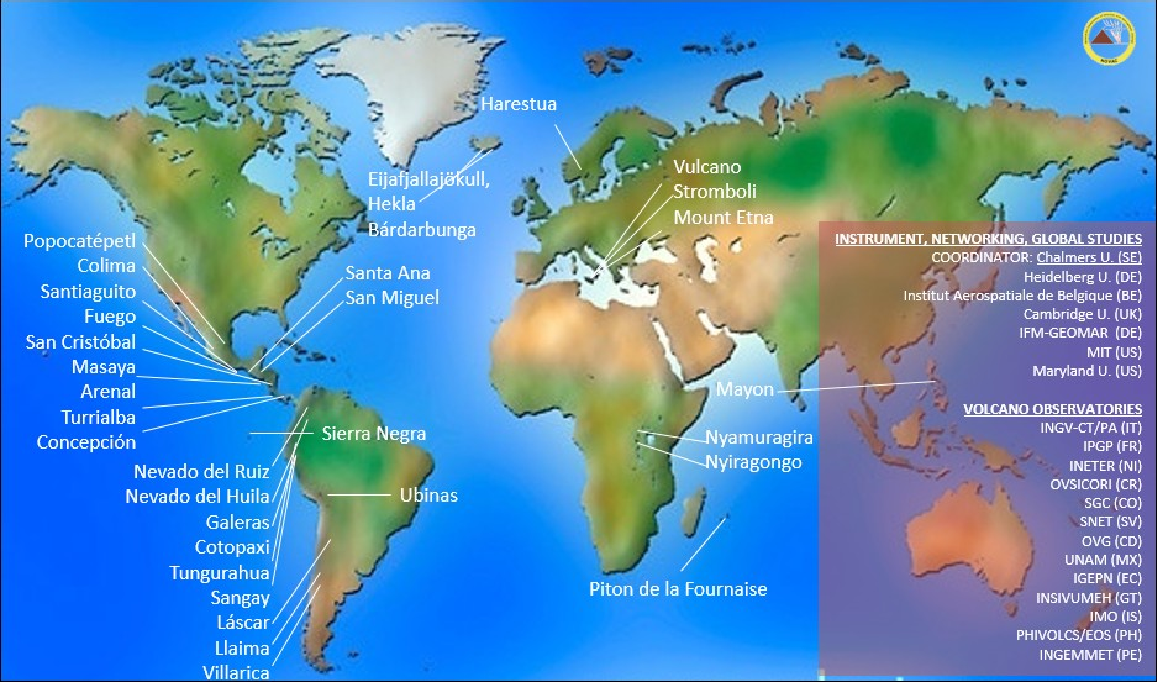
\includegraphics[width=0.8\linewidth]{Bilder/NOVAC2015}
			\caption{Global map of the volcanoes monitored by NOVAC. Used with friendly permission of Santiago Arellano.}
			\label{fig:novac2015}
		\end{figure}
		Network for Observation of Volcanic and Atmospheric Change (NOVAC) is a network of instruments monitoring volcanoes over the whole world. 
		%
		The aim of NOVAC is to gain another tool for risk assessment, for gas emissions and geophysical researches. Also many other scientific purposes are build on the data from NOVAC.\\
		%
		NOVAC was originally funded by the European Union on the first October in 2005. The aim of NOVAC is to  establish  a  global  
		network  of  stations  for  the  quantitative  measurement  of  volcanic gas  emissions. At the beginning, NOVAC encompassed observatories of 15 volcanoes in Africa America and Europe, including some of the most active and strongest degassing volcanoes in the world. Although the EU-funding has stopped, the network has been constantly growing since it was founded. In 2017 more than 80 Instruments are installed at over 30 volcanoes in more than 13 countries.
		\Cref{fig:novac2015} shows a map, with all volcanoes of the Network for Observation of Volcanic and Atmospheric Change.\\
		
		The great advantage of the data monitored in NOVAC is the fact
		that NOVAC provides continues gas emission data over many years. This ensures statistically meaningful results for the data evaluation.\\
		The instruments used in NOVAC are scanning UV-spectrometer named Mini Doas instruments. \\
		The  Mini DOAS  instrument  represents  a  major  breakthrough  in  volcanic  gas	monitoring as it is capable of real-time semi-continuous unattended measurement of the total emission fluxes of  \ce{SO2} and BrO from a volcano. Semi-continues in this case means that the measurement is only possible during daytime when enough Sunlight is there.\\
		%
		\begin{figure}
			\subfigure[Bezeichnung der linken Grafik]{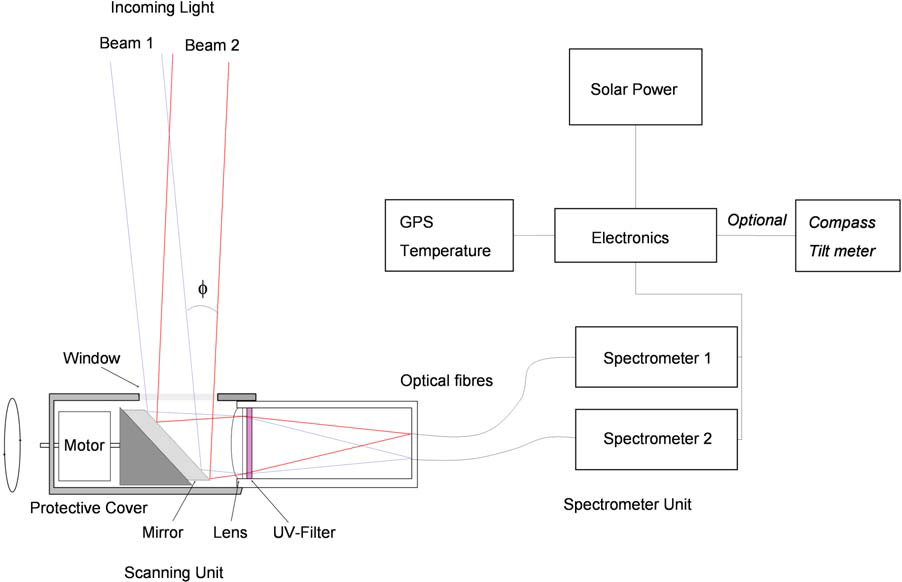
\includegraphics[width=0.49\textwidth]{Bilder/Simon/Bilder_Tung/NOVAC_Instrument}}
			\subfigure[Bezeichnung der rechten Grafik]{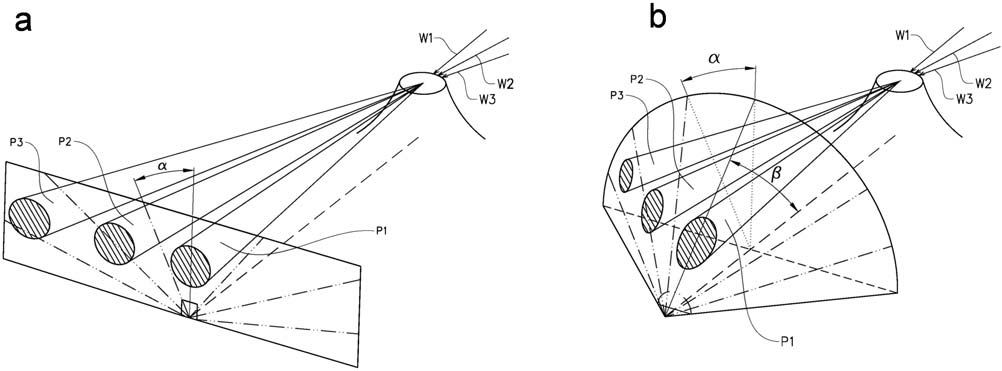
\includegraphics[width=0.49\textwidth]{Bilder/Simon/Bilder_Tung/NOVAC_scan_geo}}
			\caption{Titel unterm gesamten Bild}
		\end{figure}
		The  basic  Mini DOAS  system  consists  of  a  pointing  telescope  fiber-coupled  to  a  spectrograph.  
		Ultraviolet light from the sun, scattered from aerosols and molecules in the atmosphere, is collected by 
		means  of  a  telescope  with  a  quartz  lens  defining  a  field-of-view  of  12~mrad.
		\cite{NOVACsite} \\
		The spectrometers measure in the UV region in a wavelength range of 280 to 420~nm. In this range the differential structures of \ce{SO2} and BrO are dominant.
		\\
		The NOVAC-instruments need to be very robust to stand the conditions around volcanoes. Therefore the design of the instruments is rather simple, this means the instruments do not have internal stabilisation features like temperature stabilization to keep the measurement independent of external parameters.\\
		This comes with a reduced precision of the data, but the huge amount of data produced by NOVAC compensates for this limitation.  
		
		
		\section{Measurement Routine}
		\begin{figure}[h]
			\centering
			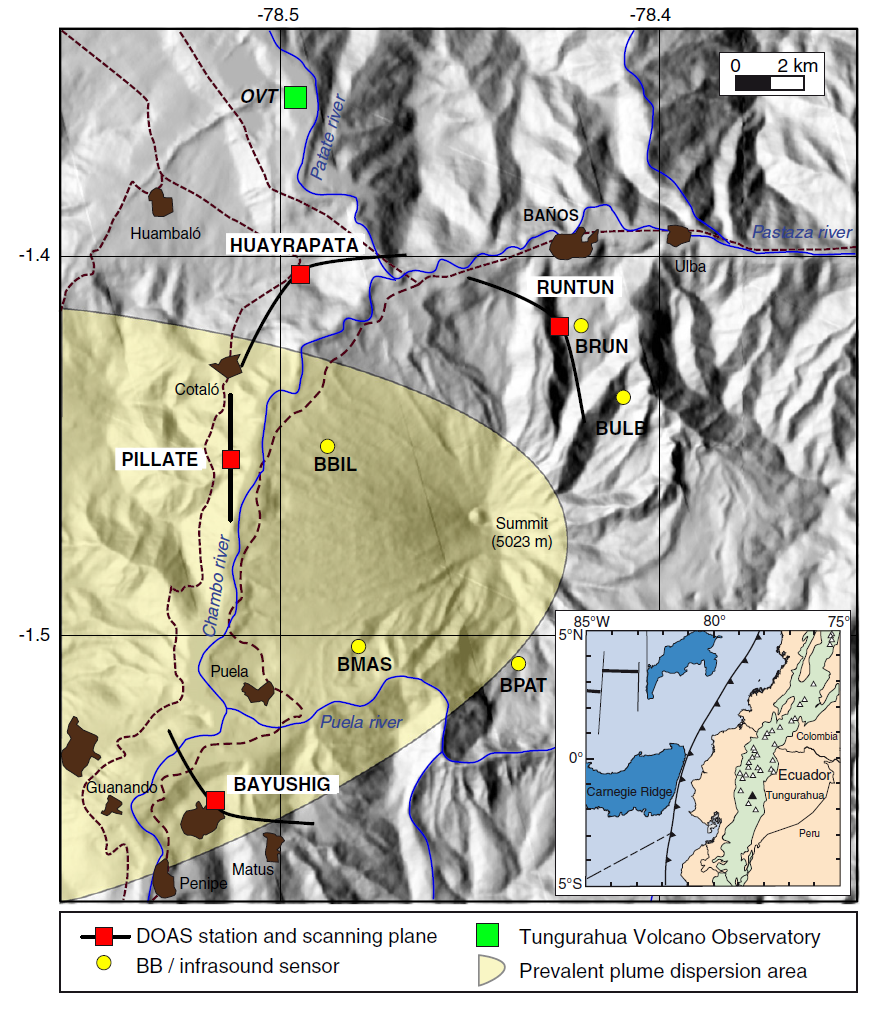
\includegraphics[width=0.6\linewidth]{Bilder/Simon/Bilder_Tung/Map_Tungurahua2}
			\caption{}
			\label{fig:maptungurahua2}
		\end{figure}
		The Instruments are set up five to ten km downwind of the volcano. To cover most of the occurring wind directions two to five instruments are installed at each volcano. Ideally, the measurement plane is orthogonal to the plume, to get the best measurement results. In reality, the measurement plane might be rotated.\\
		The Instruments record spectra in different viewing angles covering a the hole sky from horizon to horizon.\\
		The zenith is at 0$^{\circ}$.
		The measurement routine starts with a spectrum in zenith direction: the pre-reference.
		Afterwards, the dark current spectrum is recorded.\\
		Then the Instrument turns automatically to the side, recording spectra at the elevation angle from -90$^{\circ}$ to 90$^{\circ}$ with steps of 3.6$^{\circ}$. \\
		One hole measurement takes 6 to 15 minutes.
	
	\chapter{Evaluation Routine}
		\Cref{DOAS} gives an overview about the theory of the DOAS Method. This chapter will go through the algorithm which is used for the evaluation of the spectroscopic data recorded in NOVAC. 
		The occurring problem of contamination of the reference will be explained and possible solutions will be presented.
		 
	\section{NOVAC-Evaluation}
		The fitting routine used for this work is based on the DOASIS software \cite{kraus2006doasis}. 
		The equations of the DOAS retrieval of this work are slightly different from \cref{eq:taustrich}.
		\Cref{eq:lbe} can be rewritten to:
		\begin{align}
		ln\left(I\left(\lambda, L\right)\right) = &ln\left(I_0 \right) + P \left(\lambda\right) -	\int_{0}^{L}\sum_{j}\sigma_j \left(\lambda, p, T \right) \cdot c_j \left(l\right)dl \nonumber \\
		= &ln\left(I_0 \right) + P \left(\lambda\right)-
		\sum_{j}\sigma_j \left(\lambda, p, T \right) \cdot S_j
		\label{eq:lben}
		\end{align}
		%
		The term $ P \left(\lambda\right)$ is a polynomial that accounts for all broad-band effects that differ between the background spectrum $I_0\left(\lambda\right)$ and the measurement spectrum $I\left(\lambda\right)$.\\
		All Gases $j$ with relevant structures in the wavelength range used for the evaluation of SO2 (BrO) and the additional pseudo absorbers are listed in \cref{tab:gases}.\\
		The remaining task of the DOAS routing is to find a model function $F \left(\lambda\right)$ that minimizes $\chi^2$:
		\begin{equation}
		\chi^2 = \sum_{i=\lambda_1}^{\lambda_2}\left(ln(I(i))-F(i)\right)^2
		\end{equation}
		While $F\left(\lambda\right)$ can be expressed on the basis of \cref{eq:lben}:
		\begin{equation}
		F\left(\lambda\right) = ln\left(I_0 \right) + P \left(\lambda\right)-
		\sum_{j}\sigma_j \left(\lambda\right) \cdot S_j
		\end{equation}
	The DOAS fitting routine uses a combination of a standard least-squares fit and a Levenberg-Marquard algorithm to minimize $\chi^2$\\
	\\
	\begin{table}
		\begin{tabular}[|p{2cm}|p{2.5cm}|]{cc}
			\ce{BrO} Evaluation&\ce{SO2} Evaluation\\
			\toprule
			\ce{SO2}&\\
			O2&\\
			O3&\\
			O4&\\
			\bottomrule		
			\end{tabular}
			\label{tab:gases}
			\caption{All Gases used in NOVAC- Evaluation when retrieving the column densities of BrO and SO2}
		\end{table}
	
	The Network for Observation of Volcanic and Atmospheric Change provides Spectral Data for 50 different elevation angles. For the DOAS evaluation we need a reference and a measurement spectrum. To get the SCD's we need to get references without any amount of the volcanic trace gas of interest (This will be discussed more detailed in \cref{Chap:Cont}). With the so found $F\left(\lambda\right)$ the column density of  BrO and SO2 from the measurement spectrum relatively to the reference spectrum can be calculated using the calculations made above. 
	
	\begin{figure}
		\subfigure[\ce{SO2} SCD as a function of the elevation angle with error bars resulting from the DOASIS fitting routine]{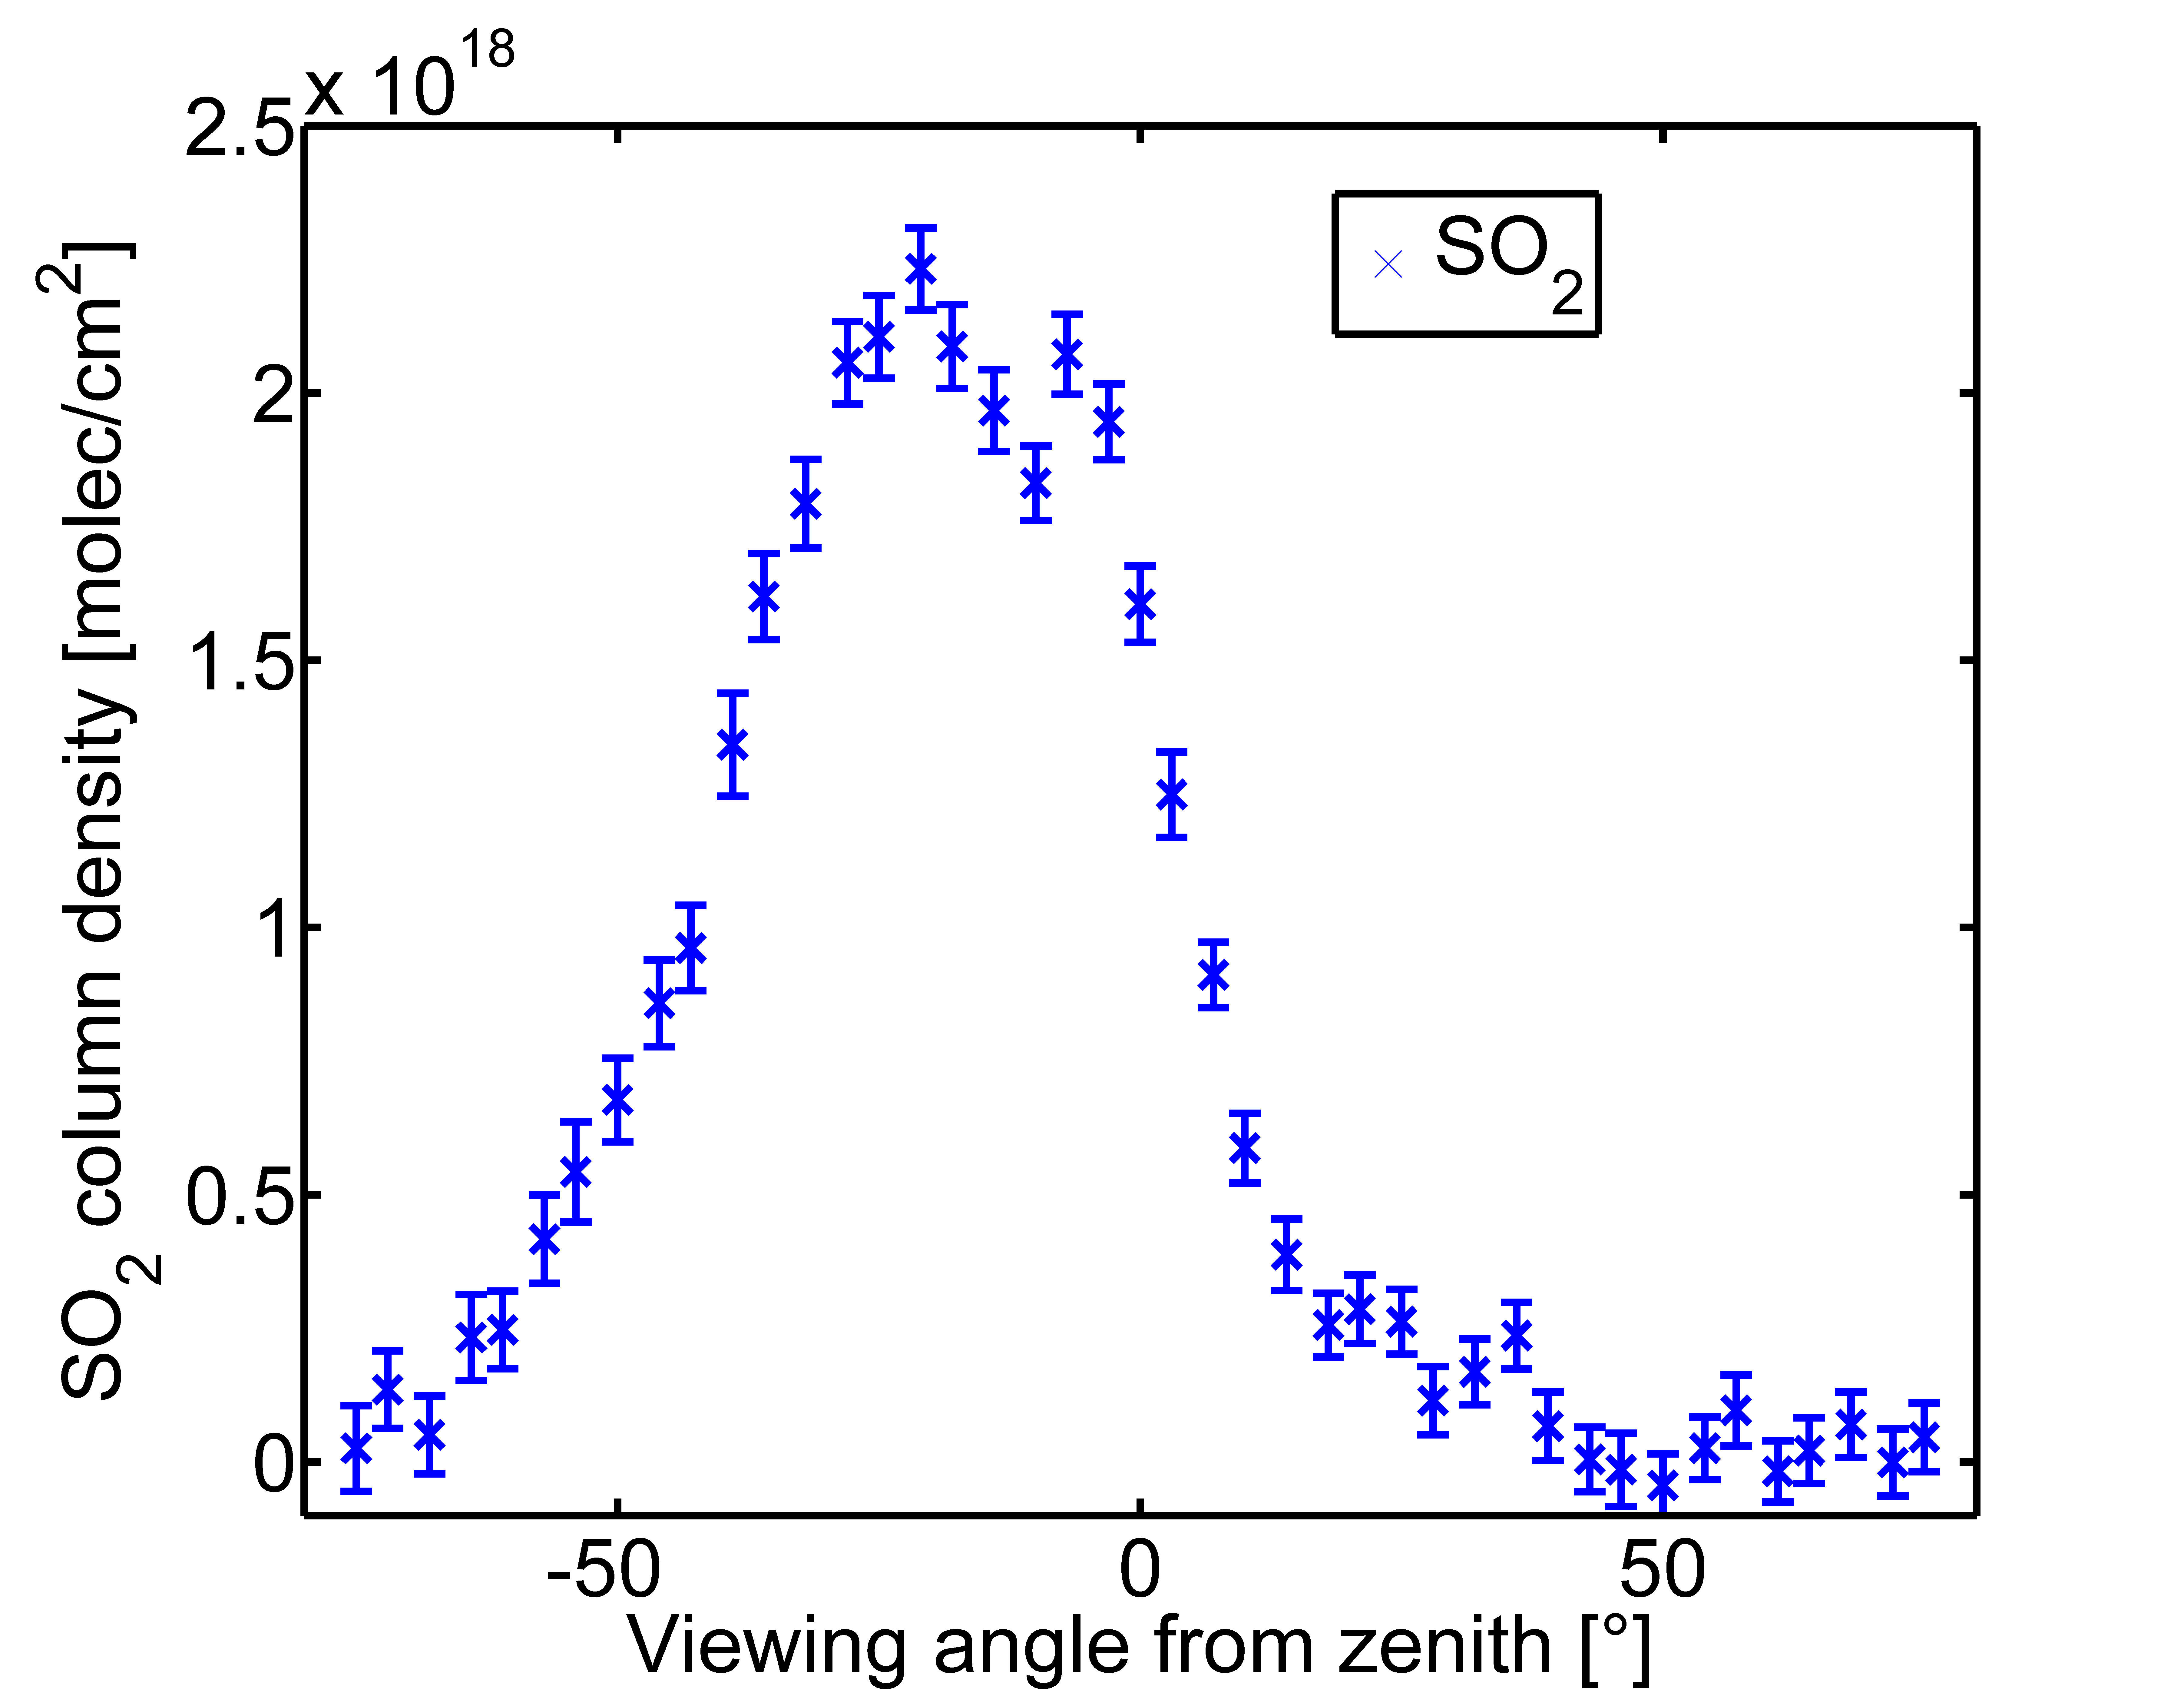
\includegraphics[width=0.49\textwidth]{Bilder/Simon/Bilder_Tung/SO2_Scan_0}}
		\subfigure[\ce{BrO} SCD as a function of the elevation angle with error bars resulting from the DOASIS fitting routine]{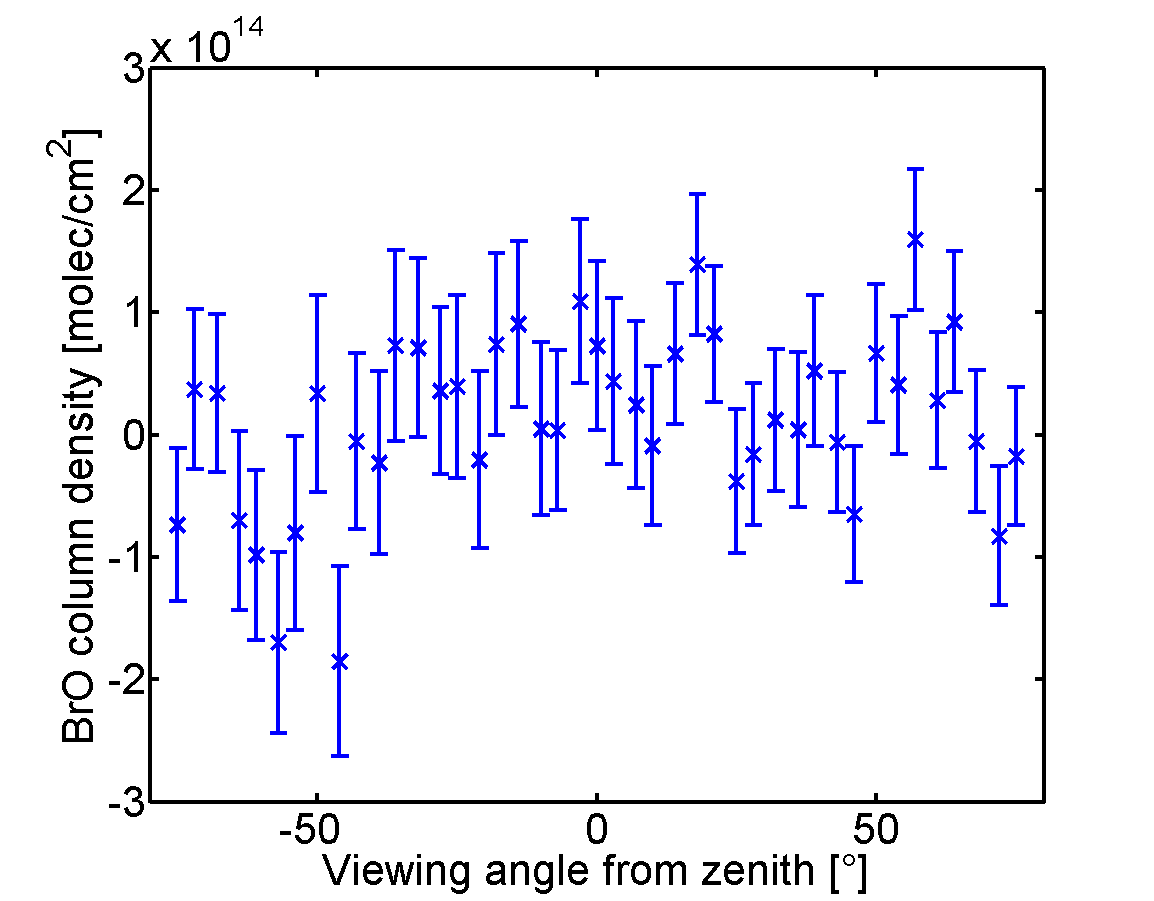
\includegraphics[width=0.49\textwidth]{Bilder/Simon/Bilder_Tung/BrO_Scan}}
		\caption{SCD's as a function of viewing angles. Adapted from \cite{WarnachSimon}}
		\label{fig:plumeref}
	\end{figure}
	%
	In the following we describe the technical implementation of the DOAS approach using the data of NOVAC instruments:\\
	\begin{figure}
		\centering
		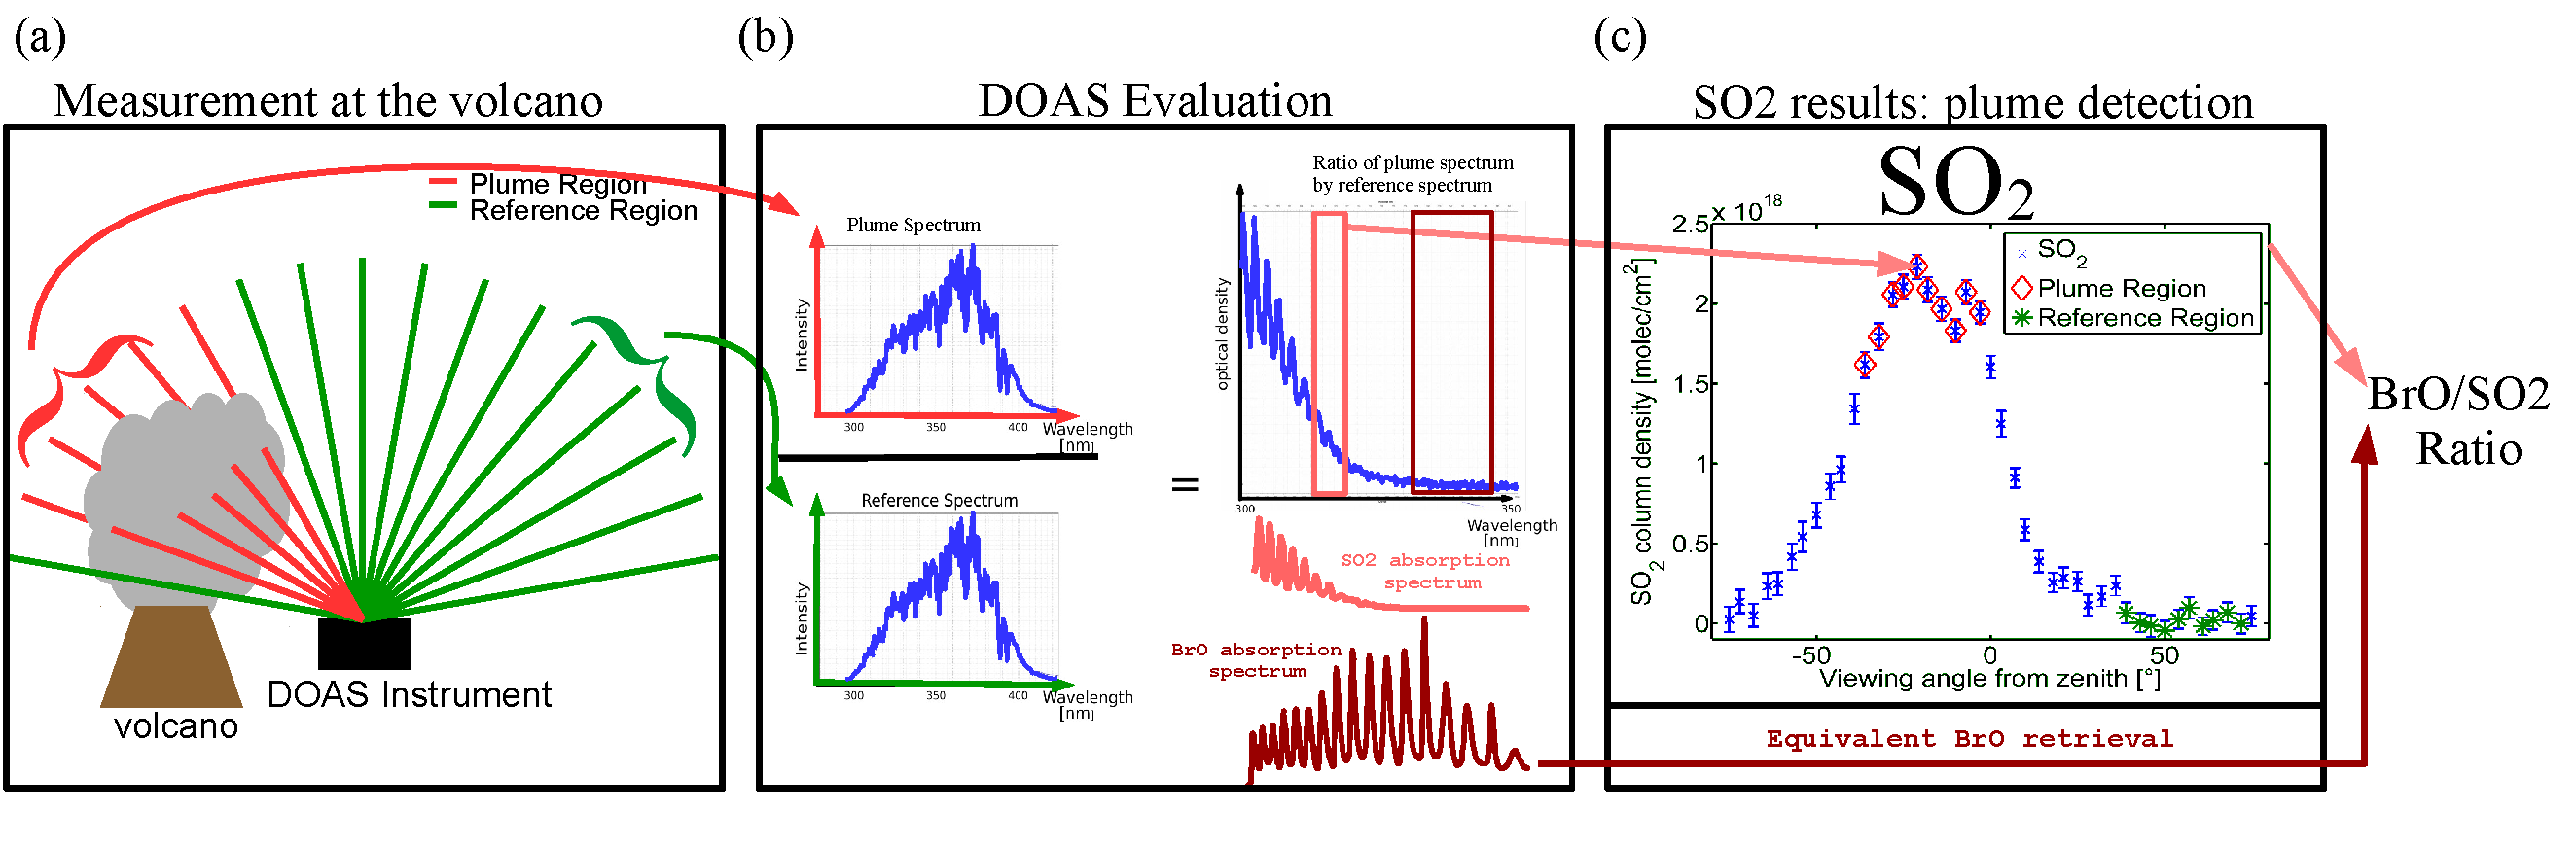
\includegraphics[width=1\linewidth]{Bilder/NOVAC_Eval}
		\caption{NOVAC Evaluation: (a) Measurement at the volcanoe (b) Evaluation of the spectral data with the DOAS routine using the absoption cross sections of BrO and SO2. (c) finding the location of the plume and reference (d) the ratios BrO/SO2 at Tungurahua }
		\label{fig:NOVAC_Eval}
	\end{figure}

	The first important task is to locate the measurement spetrum in the volcano plume and the reference region which need to be outside of the plume. 
	To do so we use the pre-reference (the spectra recorded at an elevation angle of  0$^{\circ} $) to evaluate spectra for \ce{SO2} at every elevation angle as described in chapter \ref{DOAS}, that means we divide each recorded spectra by the pre-reference and take the logarithm  to get rid of the Frauenhofer structures and to be able to just look at the important structures of the plume. The result is \ce{SO2} dSCD's as a function of the elevation angle. So we can localize the maximum and the minimum of \ce{SO2} amount, but not the SCD's.  To get the gas dSCD's of the evaluated spectra, one fits the absorption cross section of all important gases on the recorded spectrum. In our case we take all gases written in tab. \ref{tab: 1} into account.
	 Inside the plume the \ce{SO2} amount is much higher than outside the plume.  The location of the \ce{SO2} maximum match with the location of the plume. We assume that the minimum of the \ce{SO2} curve refers to a region outside of the plume which is in most times the case. The \ce{SO2} amount in the earths atmosphere is negligible so we take it as a region of zero \ce{SO2}. Now it is possible to locate the plume region as the \ce{SO2} maximum, whereas the minimum of the \ce{SO2} curve the reference region is. \\
	To technically detect the plume region we use a gauss fit of the \ce{SO2} curve.
	To increase the quality and to get a more robust result the sum over several plume spectra is taken. If the gauss curve is too wide we use only the 10 spectra with the highest \ce{SO2} amount. For the reference we use the sum of 10 spectra with the lowest \ce{SO2} amount.\\
	%
	\begin{figure}
		\centering
		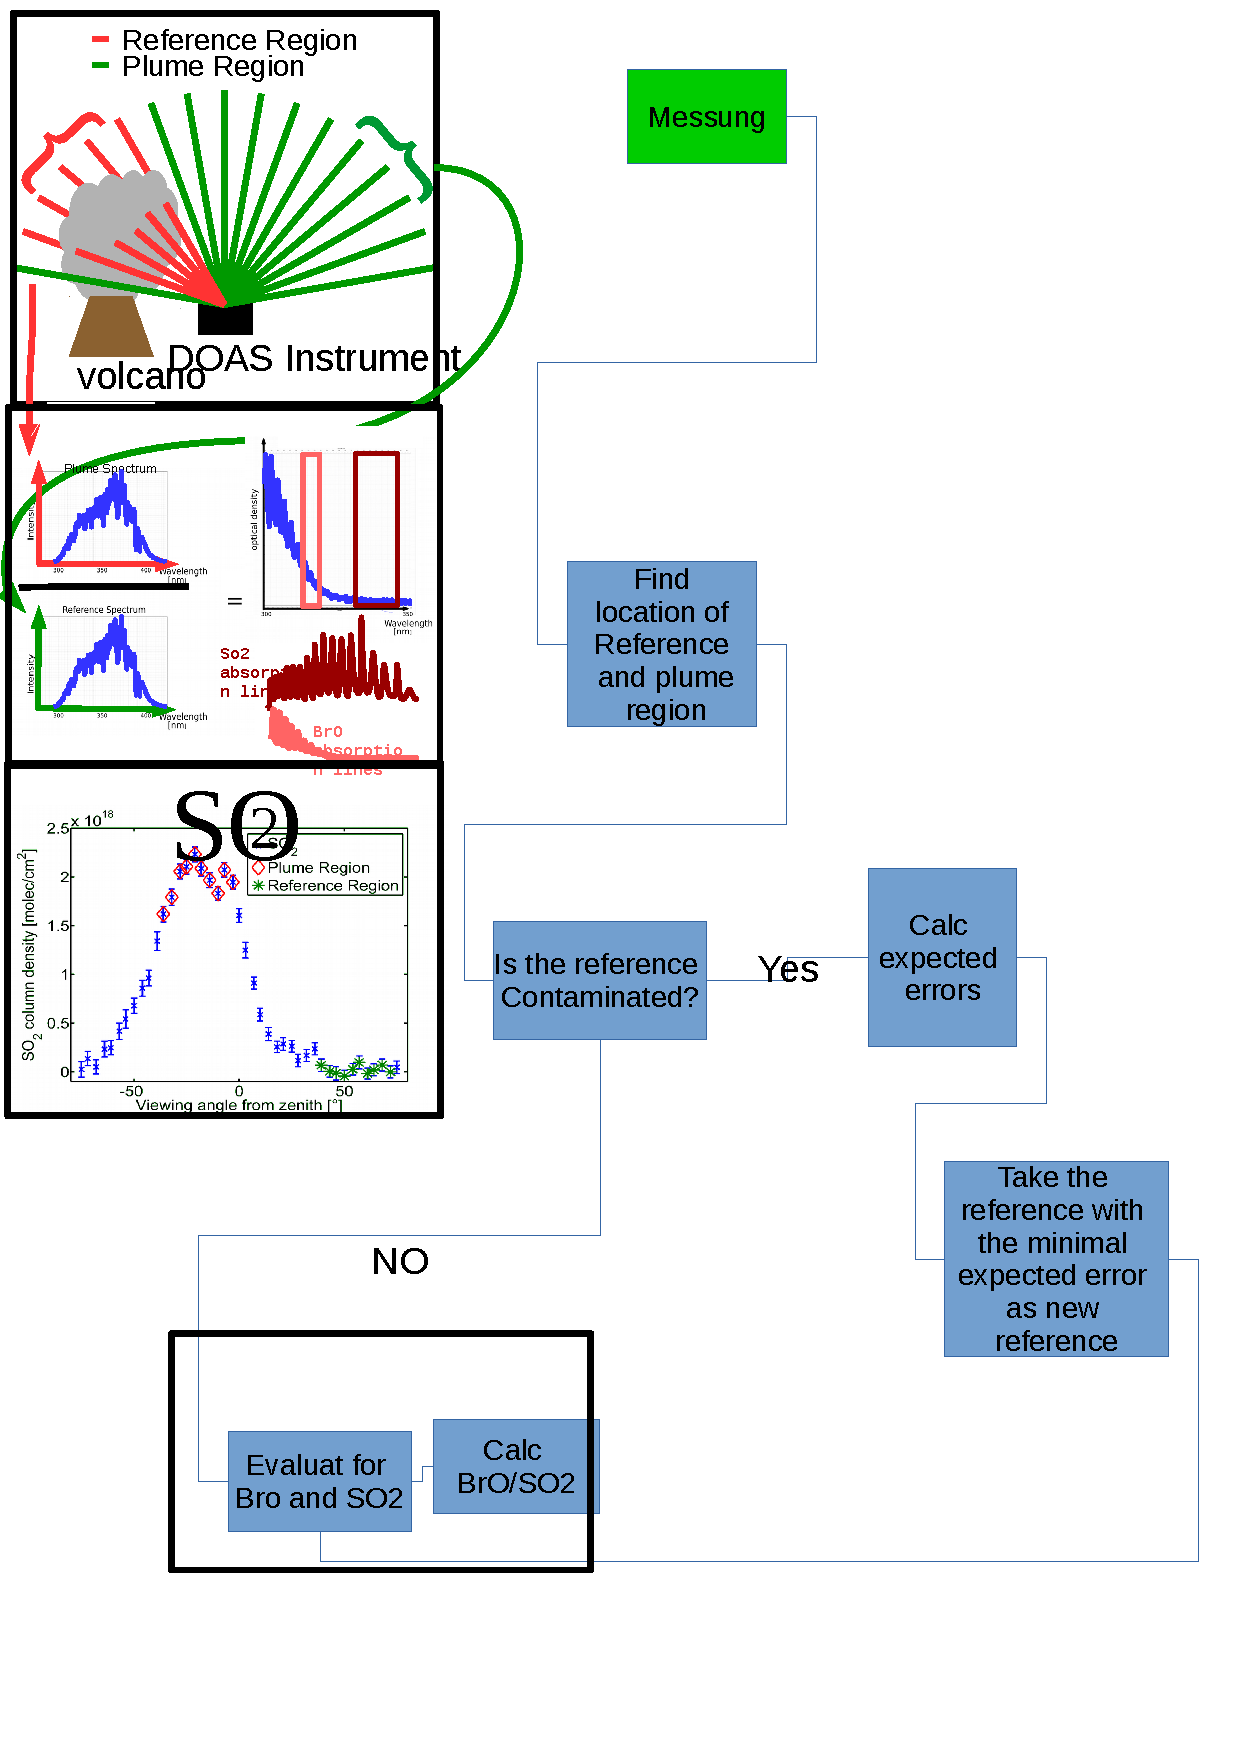
\includegraphics[width=0.7\linewidth]{Bilder/DOAS_Routine}
		\caption{Sketch of the DOAS Routine }
		\label{fig:FlussDiag}
	\end{figure}
	The so found reference spectrum is used to fit it on the \ce{SO2} absorption lines of Gases to get the absolute column densities of \ce{SO2} and \ce{BrO} in the plume spectrum\\
	In \cref{fig:plumeref} (a) the SO2 SCD as a function of the elevation angle is shown. The SO2 curve show a clear maximum at the position of the plume at an elevation angle of approximately $-30^{\circ}$ to $0^{\circ}$  and a reference region at an elevation angle of $40^{\circ}$ to $70^{\circ}$. (b): The extrema of the BrO curve are not as distinct as at the SO2 curve. \\
	Since the \ce{BrO} column density is much lower than the \ce{SO2} column density and lies just slightly above the detection limit the plume is hard to detect using the \ce{BrO} column density as it is shown in fig. \ref{fig:plumeref} (b). 
	Therefore we use plume location we found by using \ce{SO2} to evaluate the \ce{BrO} column density.\\
	For the evaluation we use the data of more than one measurement, to increase the fit quality.\\
	We are mainly interested in the \ce{BrO}/\ce{SO2} ratio, with the calculations described above it is now possible the get this ratio.
	In \cref{...} is the NOVAC Evaluation visualized.\\
	Taking the \ce{BrO}/\ce{SO2} ratio if the column densities are close to zero yields unpredictable and unrealistic results. Thus spectra measured outside of the volcano plume need to be excluded.
	This could be achieved by setting a \ce{BrO} or/and a \ce{SO2} threshold. A reasonable \ce{BrO} threshold need to be at least in the order of the DOAS fit error. But this could lead to elevated \ce{BrO}/\ce{SO2} ratios, since the \ce{BrO} error is often close to the detection limit, and thus exclude all low \ce{BrO} column densities from the evaluation.
	%
	\begin{figure}
		\subfigure[ ]{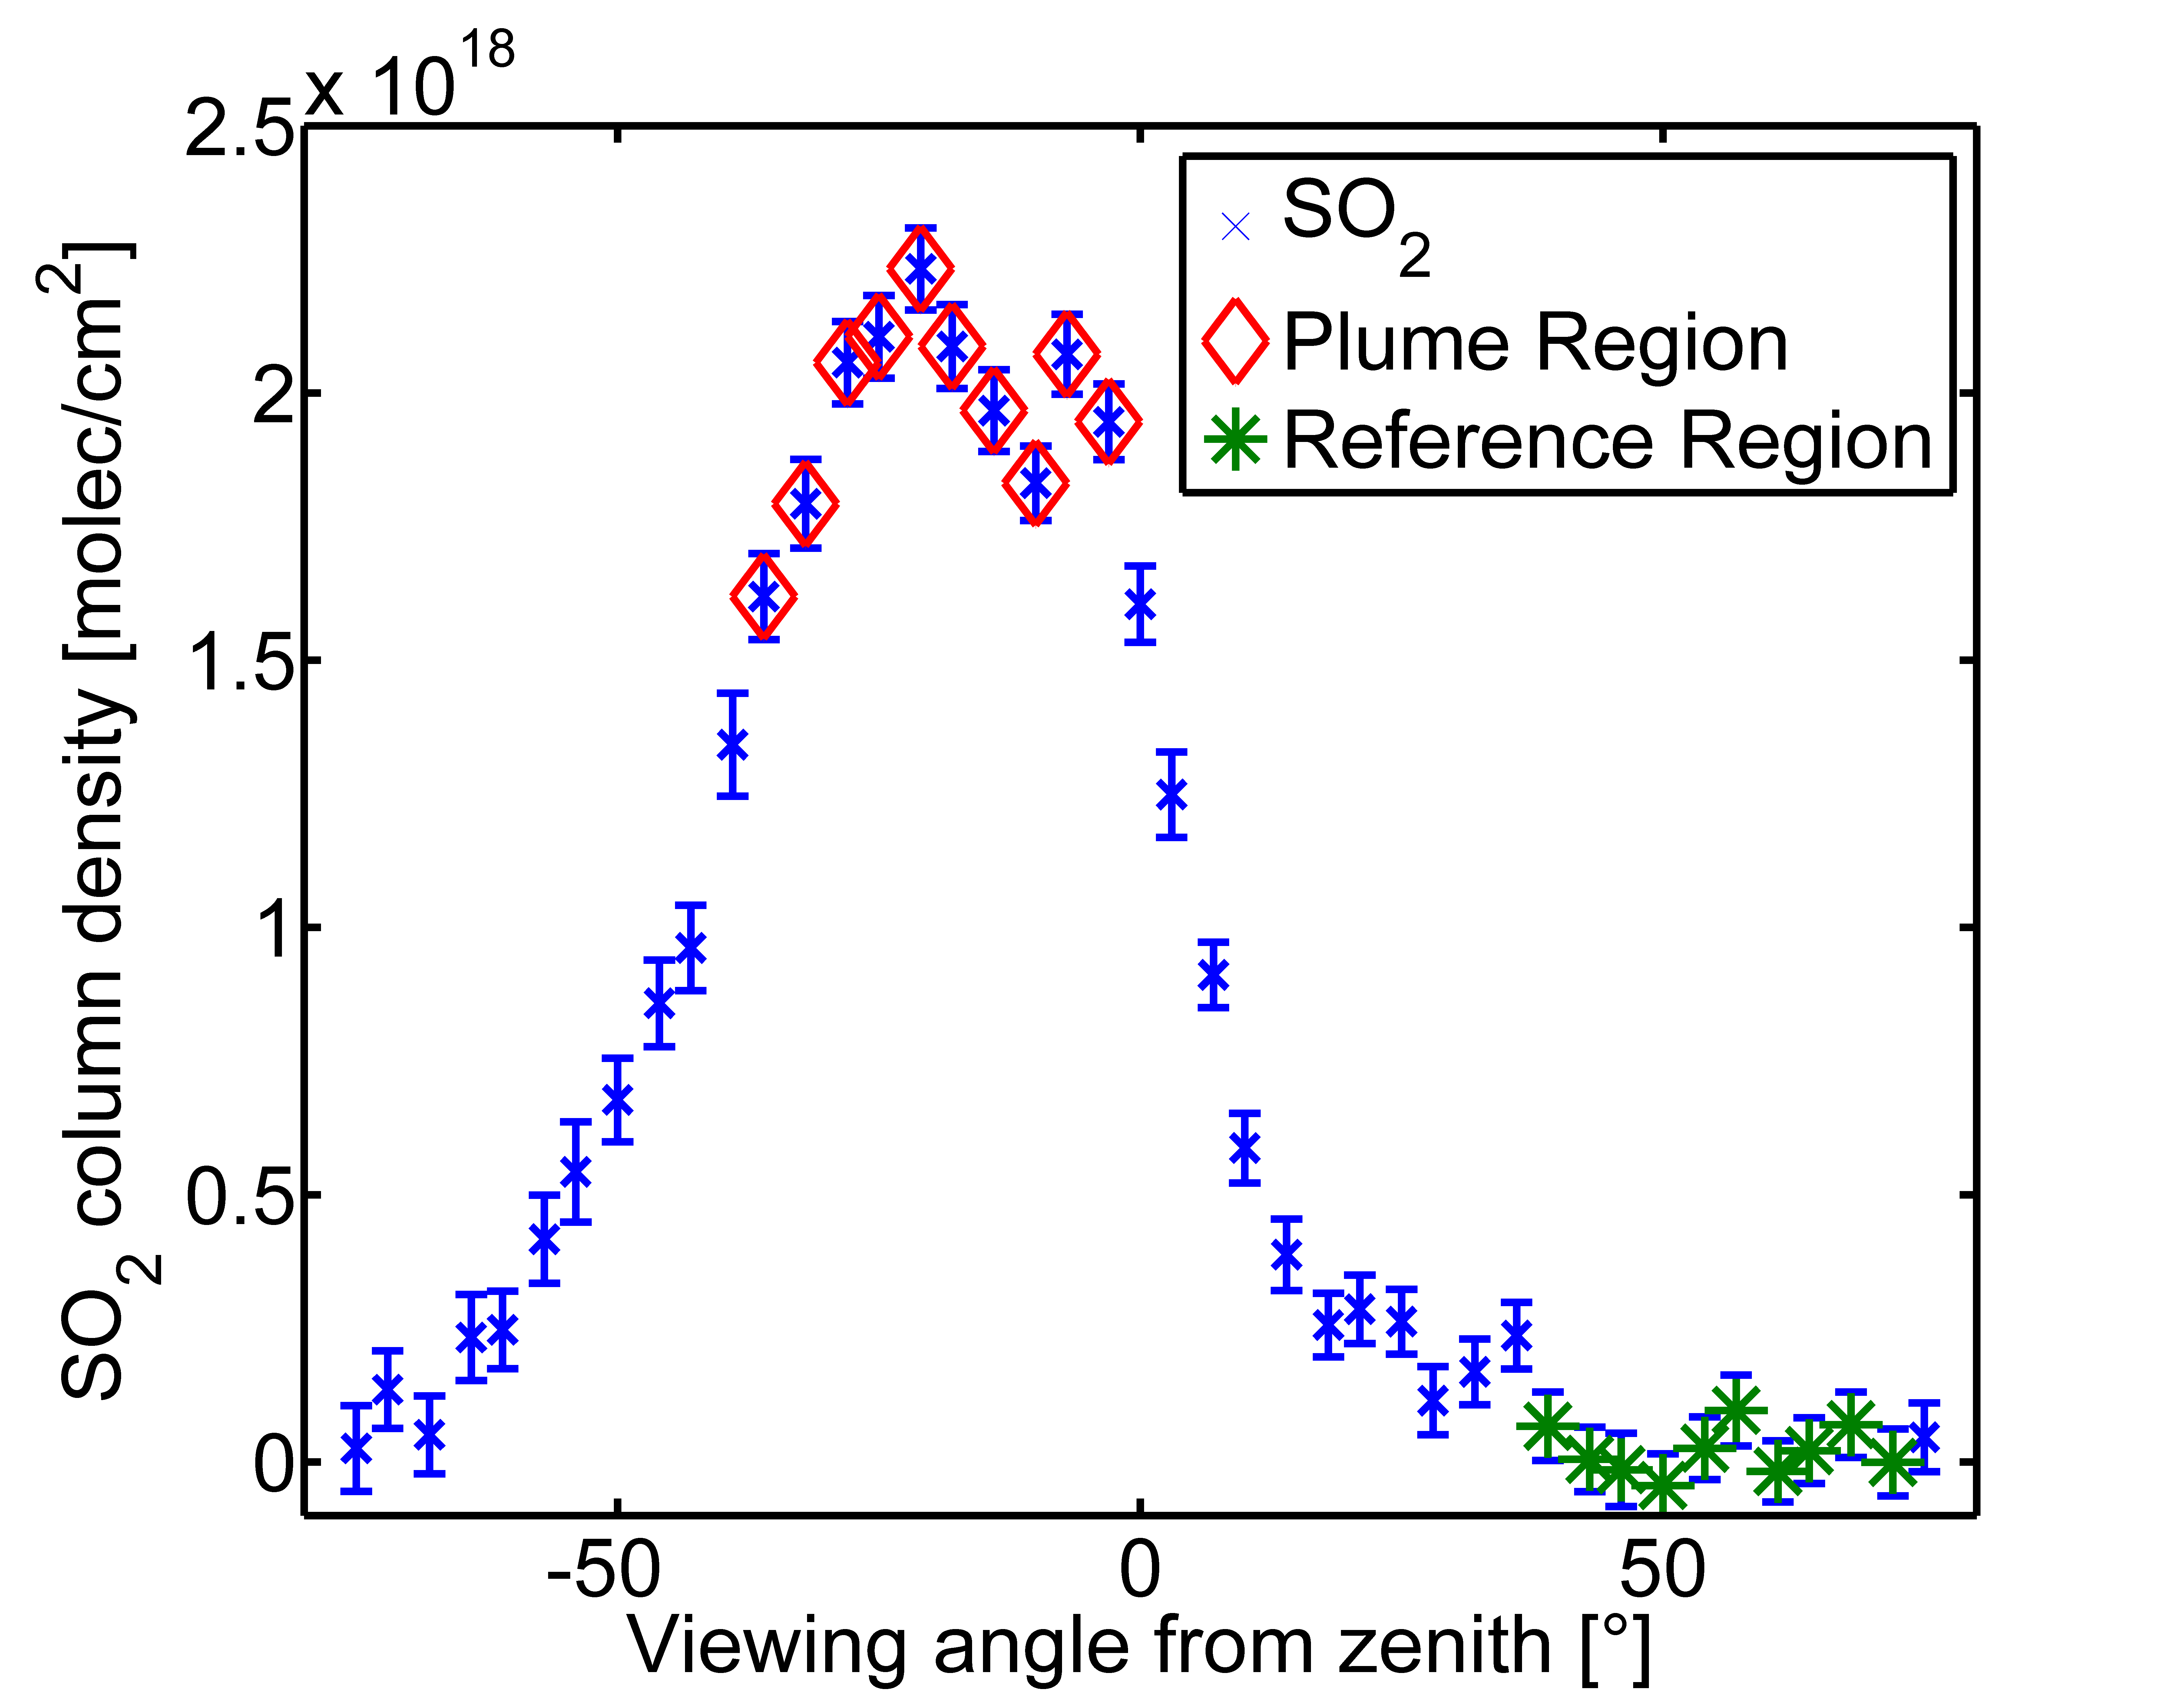
\includegraphics[width=0.5\textwidth]{Bilder/Simon/Bilder_Tung/SO2_Scan}}
		\subfigure[ ]{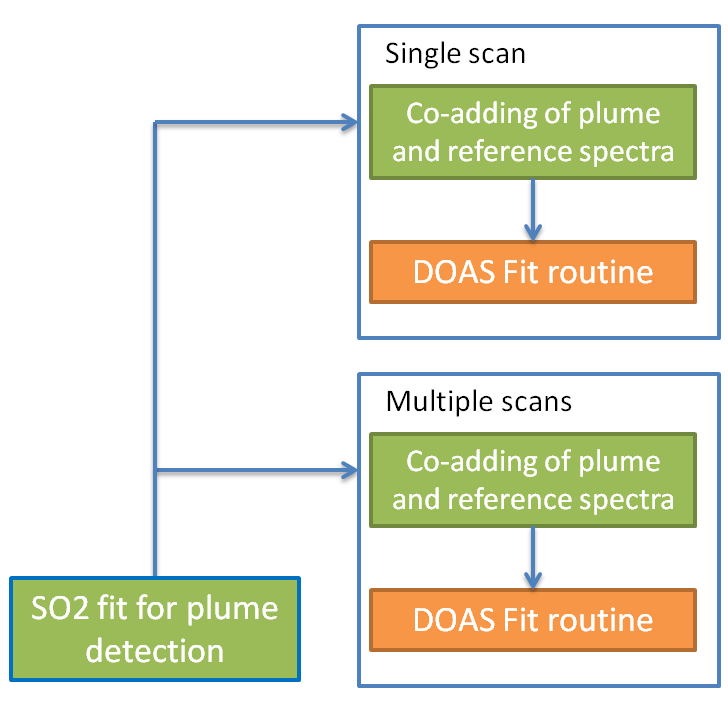
\includegraphics[width=0.47\textwidth]{Bilder/Simon/Bilder_Tung/Algorithm}}
		\caption{(a) \ce{SO2} SCD as a function of the elevation angle. The co-added Plume region is marked with red diamonds, and the co added reference region with green stars. From \cite{WarnachSimon}. (b) Flow chart of the BrO and SO2 evaluation. From \cite{lubcke2014optical}.}
		\label{fig:algorithm}
	\end{figure}
	The other possibility is to set a \ce{SO2} threshold. In this thesis an \ce{SO2} threshold of $7\cdot 10^{17} \frac{molec}{cm^2}$ was used for the selection of spectra for the evaluation of the \ce{BrO}/\ce{SO2} ratio. $7\cdot 10^{17} \frac{molec}{cm^2}$ is relatively high column density. However this this approach assures that no significant amount of gases will be filtered out, therefore the BrO/So2 will not be significantly influenced \citealp{lubcke2014bro} and that all accepted measurement spectra will be inside of the volcano plume. 
	
	\section{Contamination Problem\label{Chap:Cont}}	
	It might occur that in rare (ca. 10\% of the data) scenarios, the
	volcanic plume covers the whole scan region.
	This could happen if for example the volcanic plume of the day before still extend over the hole scan area as a consequence of windless conditions.
	In consequence, the reference	is contaminated with volcanic trace gases. Thus the gas amount is underestimated by the NOVAC-Evaluation: In \cref{fig:contaminated} we see an example from April 2011 (Tungurahua) where the reference region is contaminated by volcanic trace gases. The blue \ce{SO2} curve shows our calculations with the NOVAC-Evaluation, but since there is still \ce{SO2} in the reference region, therefore the assumption, that the \ce{SO2} amount could be set to zero in the reference region is wrong. The red curve shows the real \ce{SO2} curve, and we will underestimate the total \ce{SO2} amount of the plume. Contamination occur in approximately 10$\%$ of the data.\\
	\\
		\begin{figure}
			\centering
			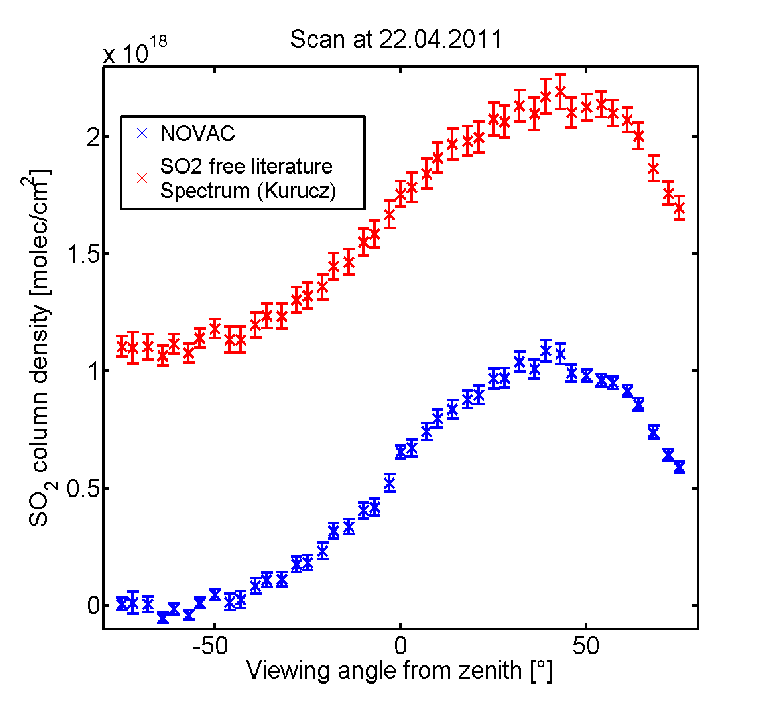
\includegraphics[width=0.7\linewidth]{Bilder/contaminated}
			\caption{Scan with a contaminated reference spectrum from April 2011. From \cite{WarnachSimon}}
			\label{fig:contaminated}
		\end{figure}
	If the reference region is for any reason
	contaminated by volcanic trace gases, the reference spectrum has to be
	replaced by a volcanic-gas-free reference. Alternative spectra are a
	theoretical solar atlas spectrum (the use of a solar atlas spectrum will be described in \cref{kuruz}) ore a a volcanic-gas-free reference
	spectrum recorded by the same instrument.\\ 
	%
	\\
	%
	In the following we will discuss both of these options:
	%
	\subsection*{Evaluation using a Solar Atlas Spectrum \label{kuruz}}
	An alternative to choose the region with the lowest column density as reference region is to use a theoretical high resolution solar atlas spectrum as reference \cite{chance2010improved}.
	The use of a theoretical solar atlas spectrum as a reference which is completely volcanic-trace-gases-free was first proposed by \cite{lubcke2014bro}.
	The advantage of using a solar atlas spectrum as reference is, that we know that there are no volcanic trace gases, we do not need to assume, that the minimum \ce{SO2} amount is zero. The disadvantage is, that using a solar atlas spectrum comes along with a drawback of precision: A theoretical solar atlas spectrum is far more precise than the spectra of the NOVAC instruments therefore the instrument functions need to be modeled and added to the retrieval.\\ 
	The reduction of precision is acceptable for the
	\ce{SO2} retrieval but not suitable for a \ce{BrO} retrieval because then most data would be below the detection limit.\\
%
\\
%
	Possible contaminations can be checked
	by a theoretical solar atlas spectrum to evaluate the \ce{SO2} amount in the reference.
	%
	\subsection*{Evaluation using a Spectrum of the same Instrument}
	An alternative reference spectrum could be a a volcanic-gas-free reference
	spectrum recorded by the same instrument. When using such a reference several problems occur:\\
	As described in \cref{NOVAC} the instruments used in NOVAC do not include features like temperature stabilisation due to that the measurements are not independent from external parameters. 
	So we need to choose a reference recorded at similar conditions with respect to meteorology and	radiation as well as in the temporal proximity due to instrumental changes with time and ambient conditions. Ideally the external conditions should be equal to the conditions when the plume was recorded.\\
	\\
	%
	\\
	In this work we will combine both options in order to
	achieve both, enhanced accuracy but still maximum possible precision of
	the \ce{SO2} and \ce{BrO} retrievals. So we use the solar atlas spectrum to check for 
	contamination and a reference spectrum recorded in temporal proximity by the same instrument as reference.\\
	\\
	%
	\\
	In the following we will discuss how to find the an optimal reference from another scan automatically.
	
	\begin{figure}
		\centering
	%	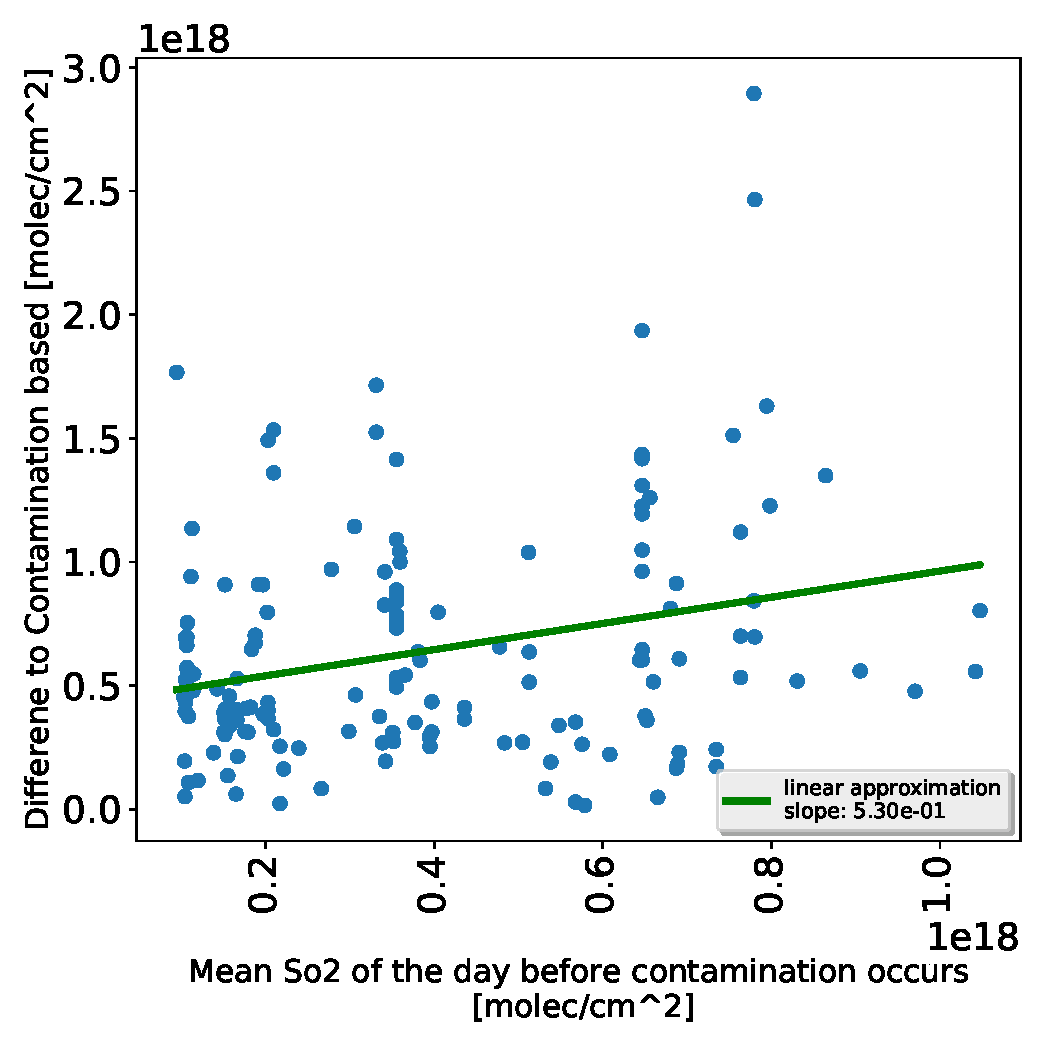
\includegraphics[width=0.7\linewidth]{E:/Masterarbeit/Analyse_Contamination/contaminationdependency_so2}
		\caption{}
		\label{fig:contaminationdependencyso2}
	\end{figure}
	\begin{figure}
		\centering
%		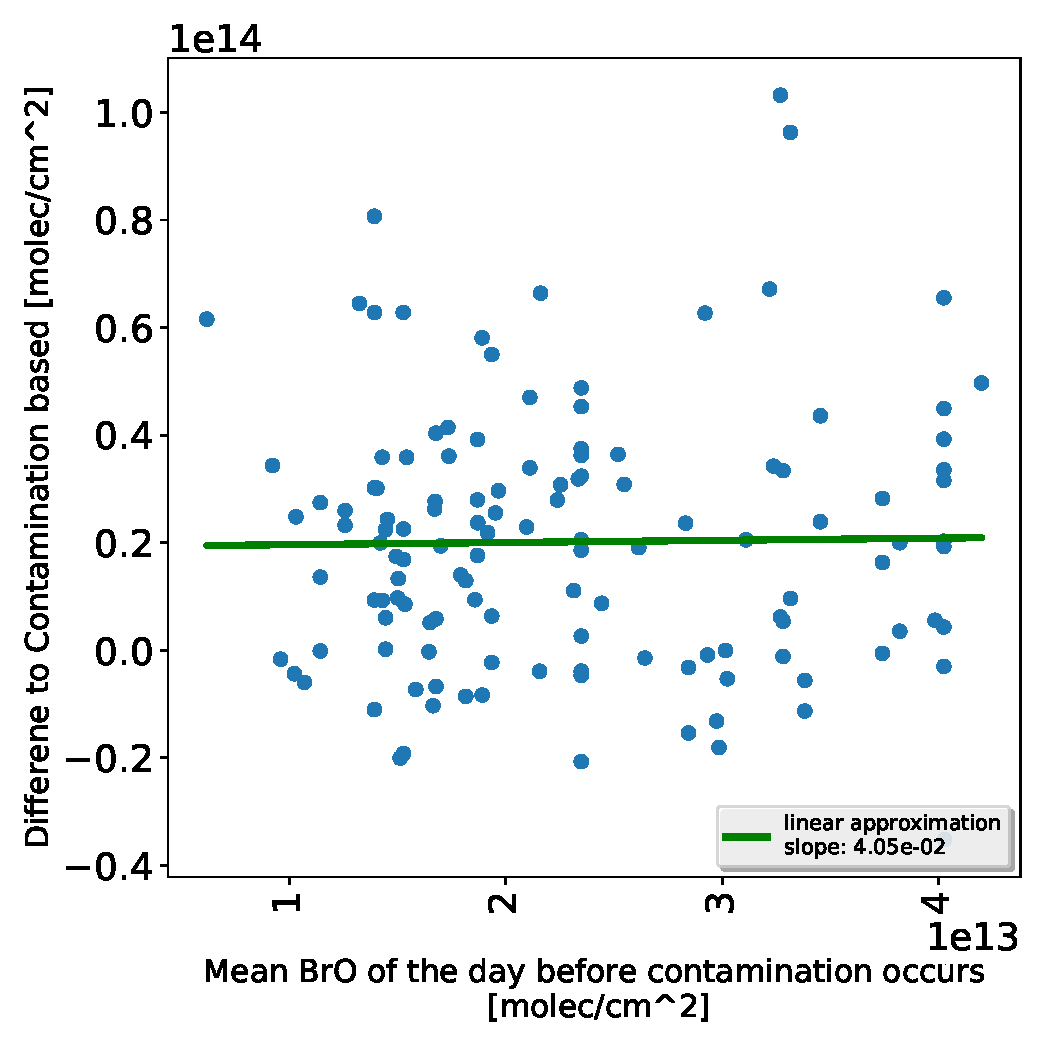
\includegraphics[width=0.7\linewidth]{E:/Masterarbeit/Analyse_Contamination/contaminationdependency_bro}
		\caption{}
		\label{fig:contaminationdependencybro}
	\end{figure}
	\begin{figure}
		\centering
%		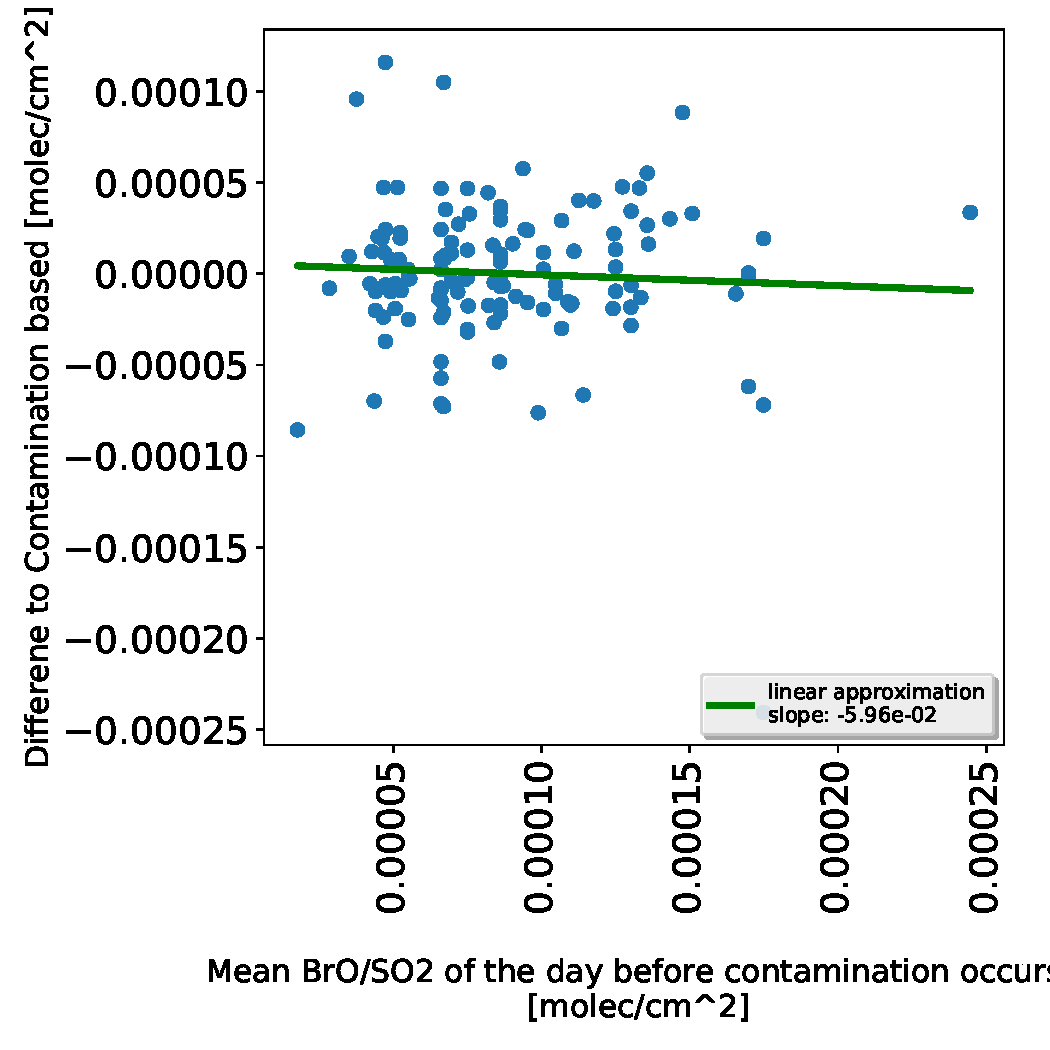
\includegraphics[width=0.7\linewidth]{E:/Masterarbeit/Analyse_Contamination/contaminationdependency_ratio}
		\caption{}
		\label{fig:contaminationdependencyratio}
	\end{figure}
	\chapter{Limitations for the evaluation of  BrO}
    Since the \ce{SO2} amount in a volcano plume is rather high (magnitude of \ce{SO2} at Tungurahua $\approx 1e^{18}$, \cite{WarnachSimon}) , the evaluation of \ce{SO2} is unproblematic compared to BrO.\\
	Evaluating \ce{BrO} is more difficult since the amount is much smaller and the measurement error relative to the column density much larger. Since we want to get the \ce{BrO}/\ce{SO2} we need to maximize the accuracy of BrO.
	Therefore the aim is to choose the reference with respect to the \ce{BrO} error, to minimize the \ce{BrO} Error and to increase the amount of reliable \ce{BrO}/\ce{SO2} ratio data.\\
	We figured out, that the \ce{BrO} Error depends strongly on the surrounding conditions when recording the plume and the reference. In the following, we will take a closer look at the dependence of the \ce{BrO} error on external parameters. 
	%
	\section{\ce{BrO} Error dependence on external parameters \label{Chap:BROErr}}
	%HOW IS THE ERROR CALCULATED AND WHY AND DETECTION LIMIT (PLATT \& STUTZ)
	The measurement and evaluation depends on the surrounding conditions like temperature or cloudiness \cite{lubcke2014optical}\\
	If choosing a new reference we need to take the surrounding conditions into account\\
	The better the surrounding conditions of the time where the reference is measured coincide with the conditions of the time when the plume is measured, the lower is the \ce{BrO} error \\
	The surrounding conditions we take into account are temperature, colorindex, exposure time, elevation-angle, daytime and the temporal difference.\\
	In almost all cases (99\%) the absolute \ce{BrO} Error is minimal when using the reference recorded at the same time as te plume spectrum. So we won't be able to get an \ce{BrO} Error which is smaller than the "Same Time Error".   

	
	\subsection{Time}
	Due to instrument drifts the fit quality decreases with the time difference between recording the plume and the reference. Therefore it is better to use an reference in temporal proximity.\\
	%
	\begin{figure}[h]
		\centering
		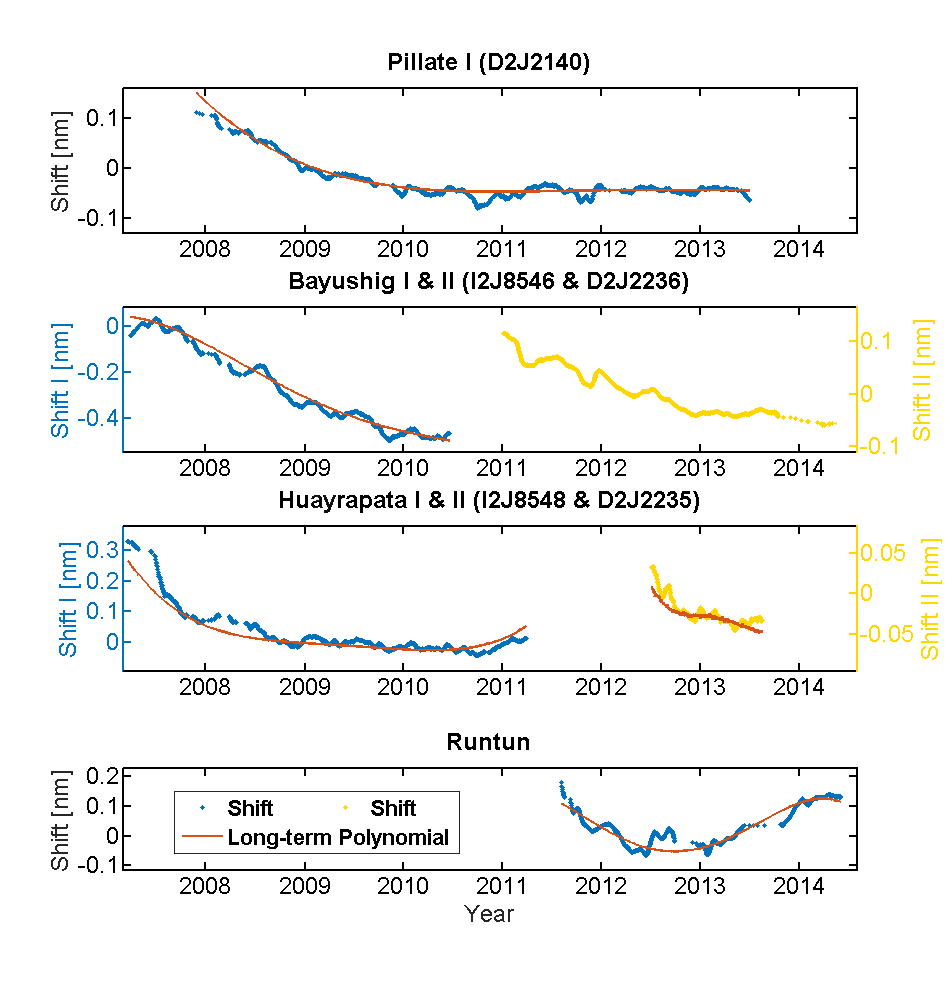
\includegraphics[width=0.7\linewidth]{Bilder/Simon/Bilder_Tung/Drift_Komplett_NEW}
		\caption{}
		\label{fig:driftkomplettnew}
	\end{figure}
	%
	\Cref{fig:driftkomplettnew} shows the instrumental drift as a function of time, to create \cref{fig:driftkomplettnew} we used Tungurahua data, 2008 from June to November. We can observe that the drift changes with time. If we use the reference and plume spectra of the same time, we do not need to care about these effects, since the shift is equal for the plume and reference spectrum, but if the recording time is not the same the quality of the fit changes with the differences in wavelength shift which increases with the time difference.\\
	In \cref{fig:dat} the \ce{BrO} Error as a function of the time difference between recording the plume and the reference is shown. The running mean is drawn with a black line. The \ce{BrO} Error increases with time difference.\\
	To evaluate the maximal time difference, were we still get reliable results we calculated for all possible reference-plume pairs the corresponding \ce{BrO} Error. With this data we are able to find for all plume spectra the associated reference where the \ce{BrO} Error is minimal. In \cref{Histogram} a histogram is plotted with the probability of picking the best reference as a function of the time difference. Obviously the best results are if the day of measuring the reference is the same day as measuring the reference that means, if the time difference is smaller than one day. We allow all time difference which are in one sigma area. 
	
	We found out that the time interval where it is still reasonable to use references is about 14 days. Therefore we only use references where the recording time difference between plume and reference is smaller than two weeks. When using a references with a temporal difference to the plume of more than 14 days the probability, that the fit quality and thus the \ce{BrO} error increases to much for our purposes. \\
	\\
	\begin{figure}
		\centering
		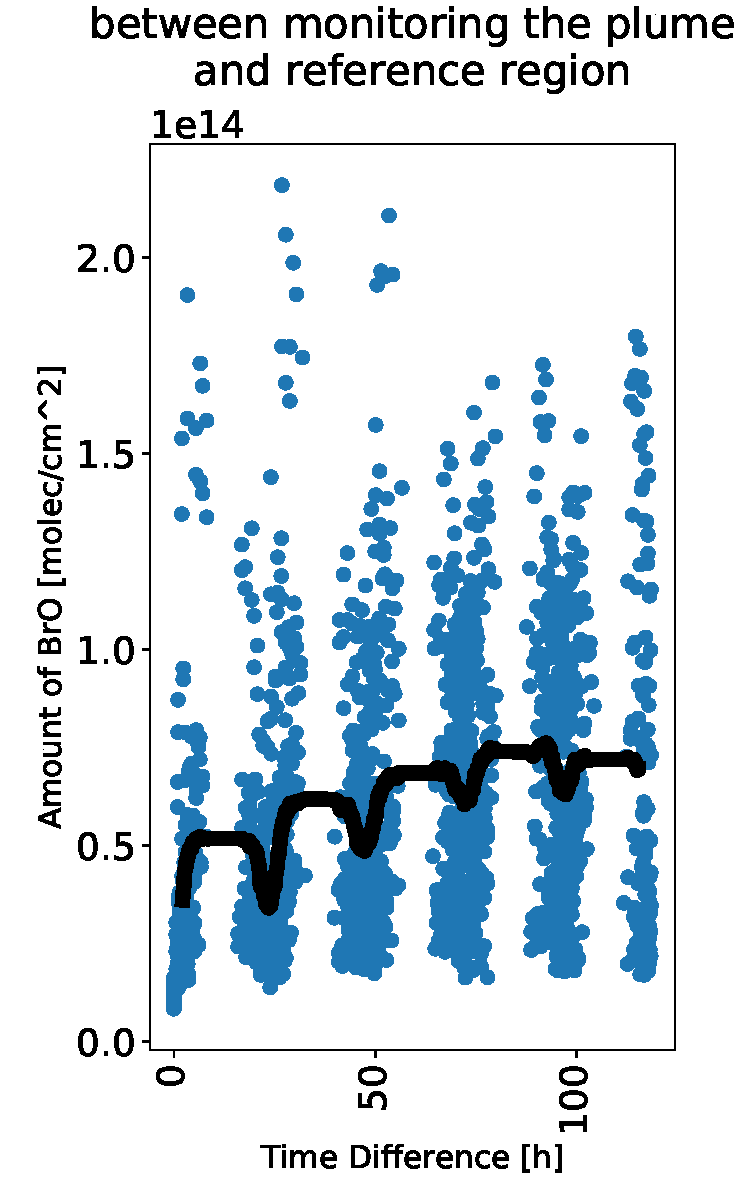
\includegraphics[width=0.7\linewidth]{Bilder/Datum_100h}
		\caption{}
		\label{fig:datum100h}
	\end{figure}	
	\begin{figure}[h!]
		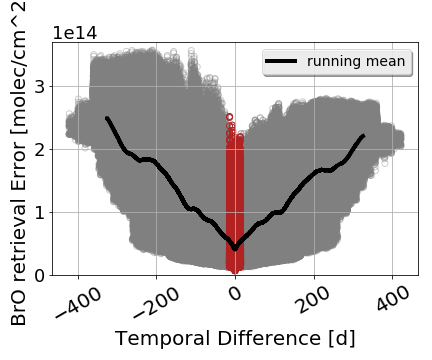
\includegraphics[width=1.1\linewidth]{Bilder/Datum}
		\caption{}
		\label{fig:dat}
	\end{figure}
	%
	\begin{figure}[h!]		
		\subfigure[Data of Tungurahua]{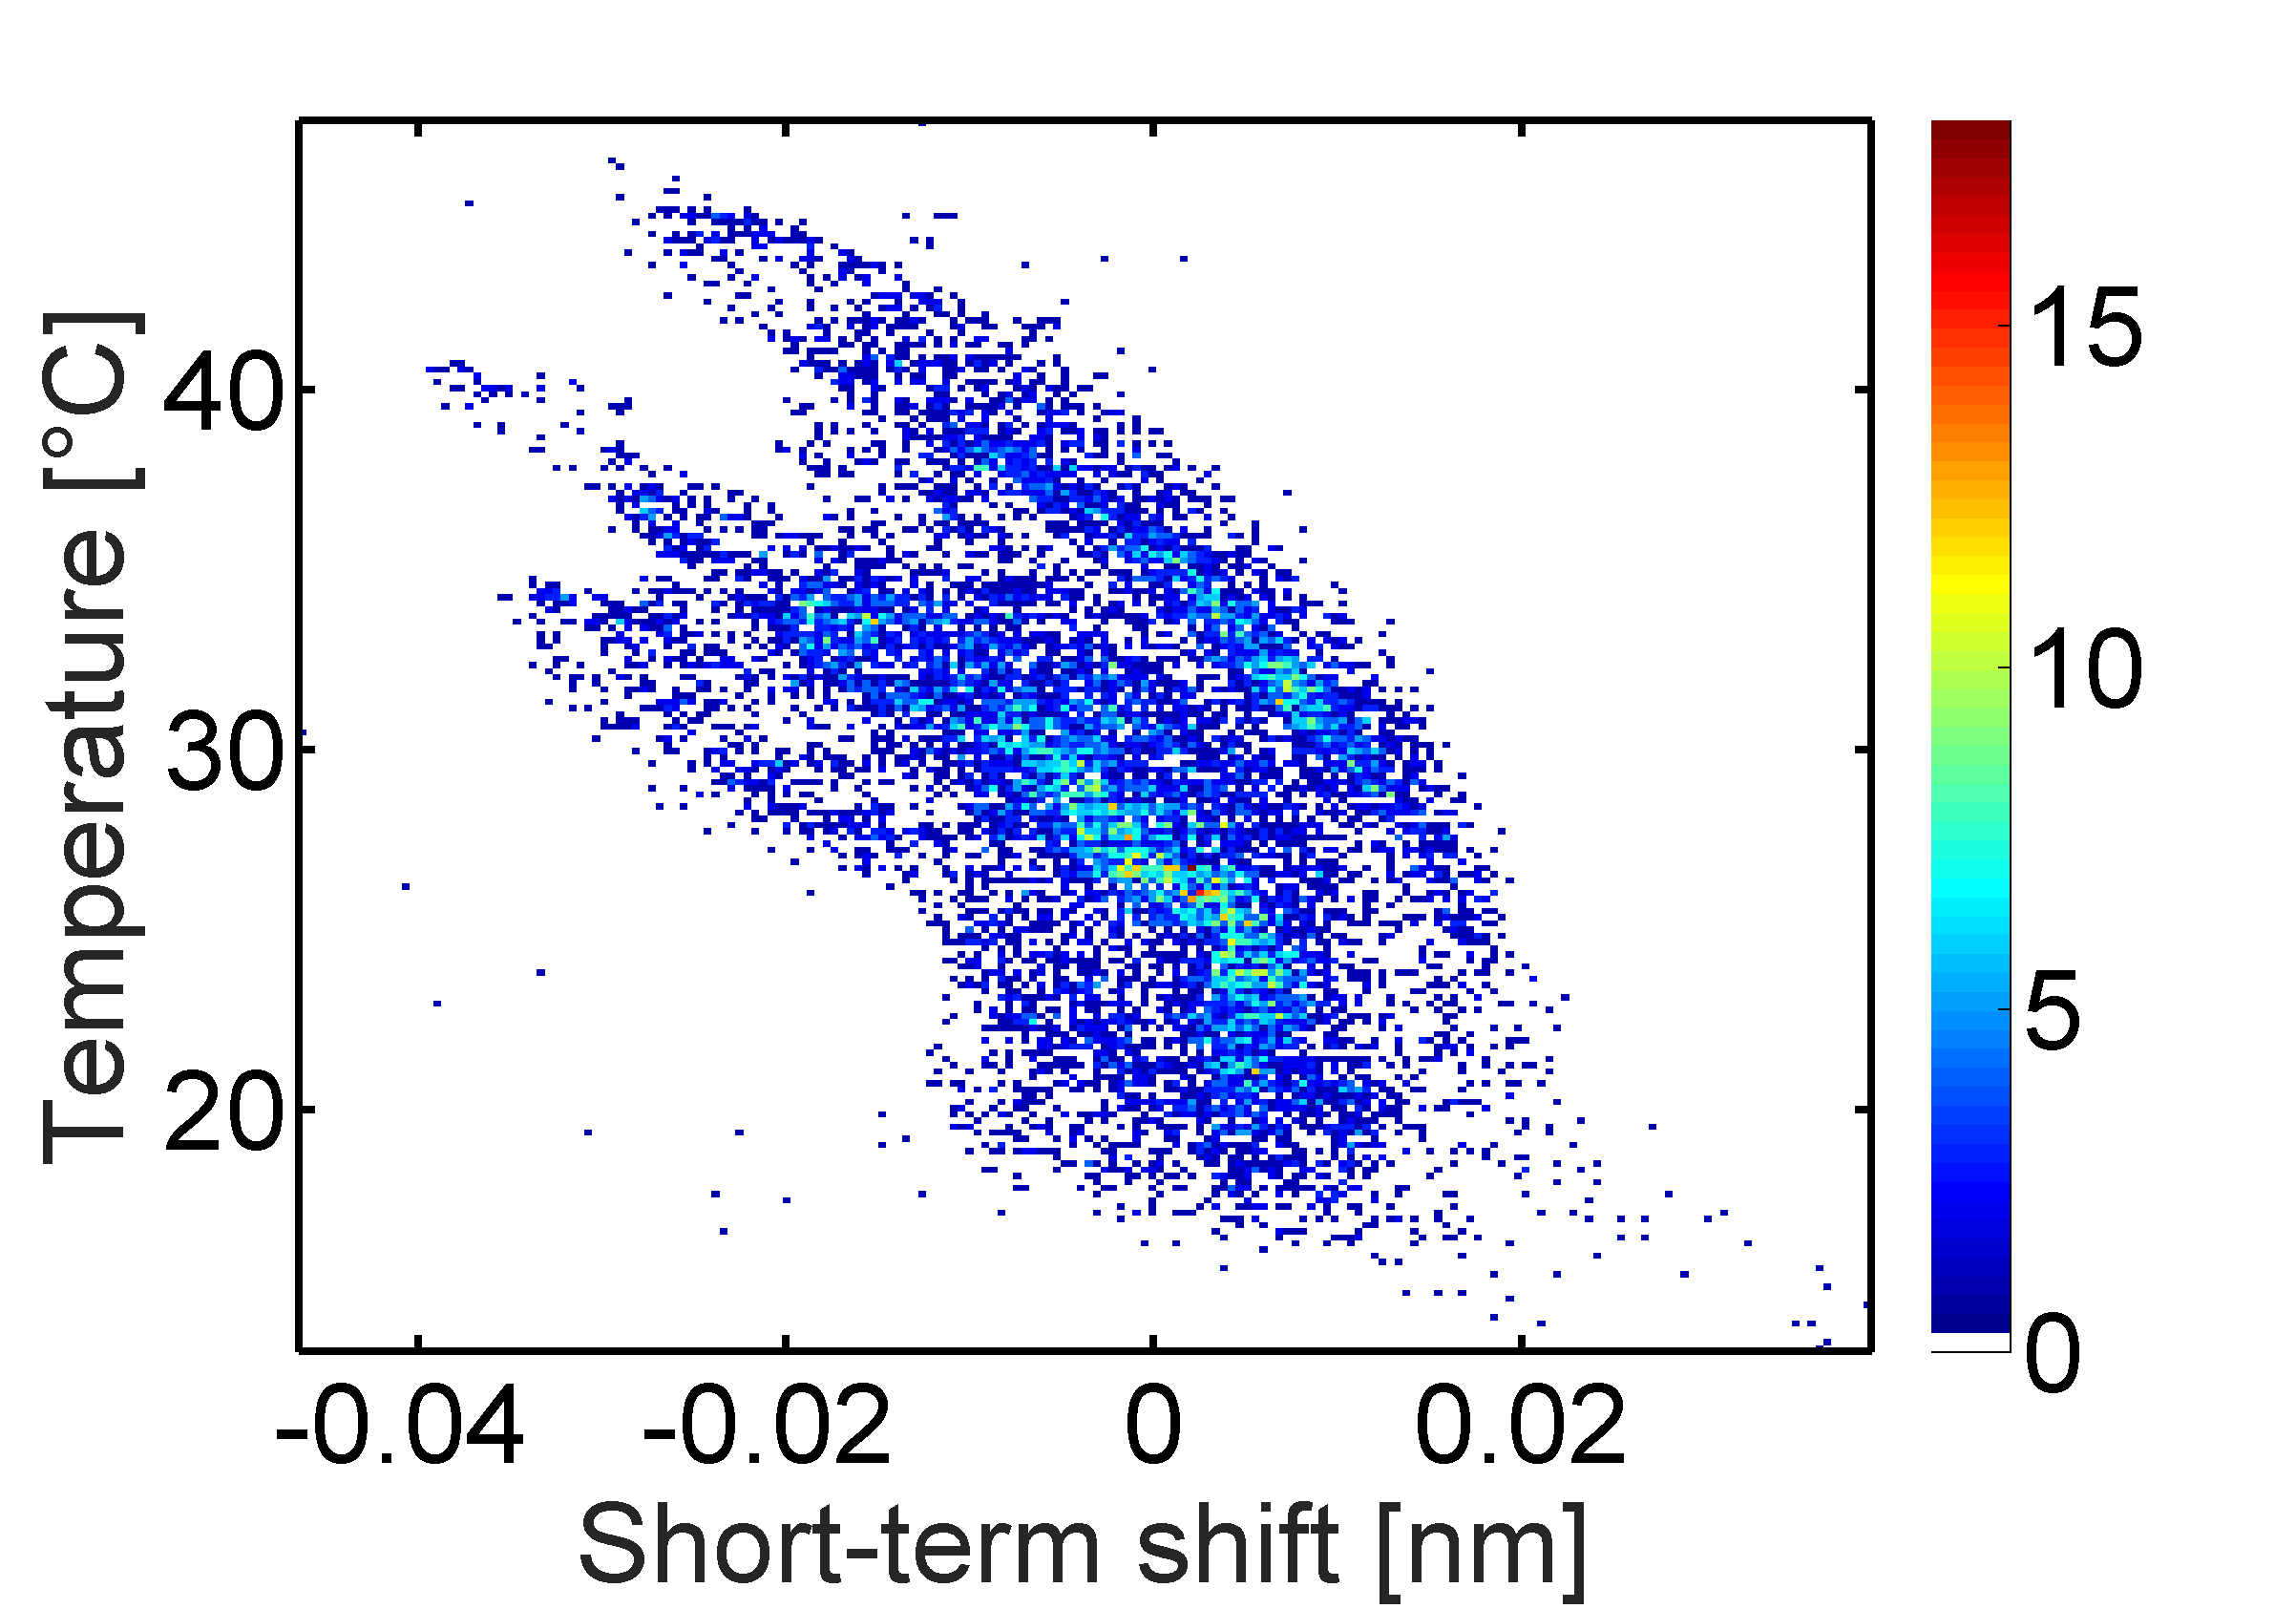
\includegraphics[width=0.49\textwidth]{Bilder/Simon/Bilder_Tung/D2J2140_Before}}
		\subfigure[Data of Nevado Del Riz]{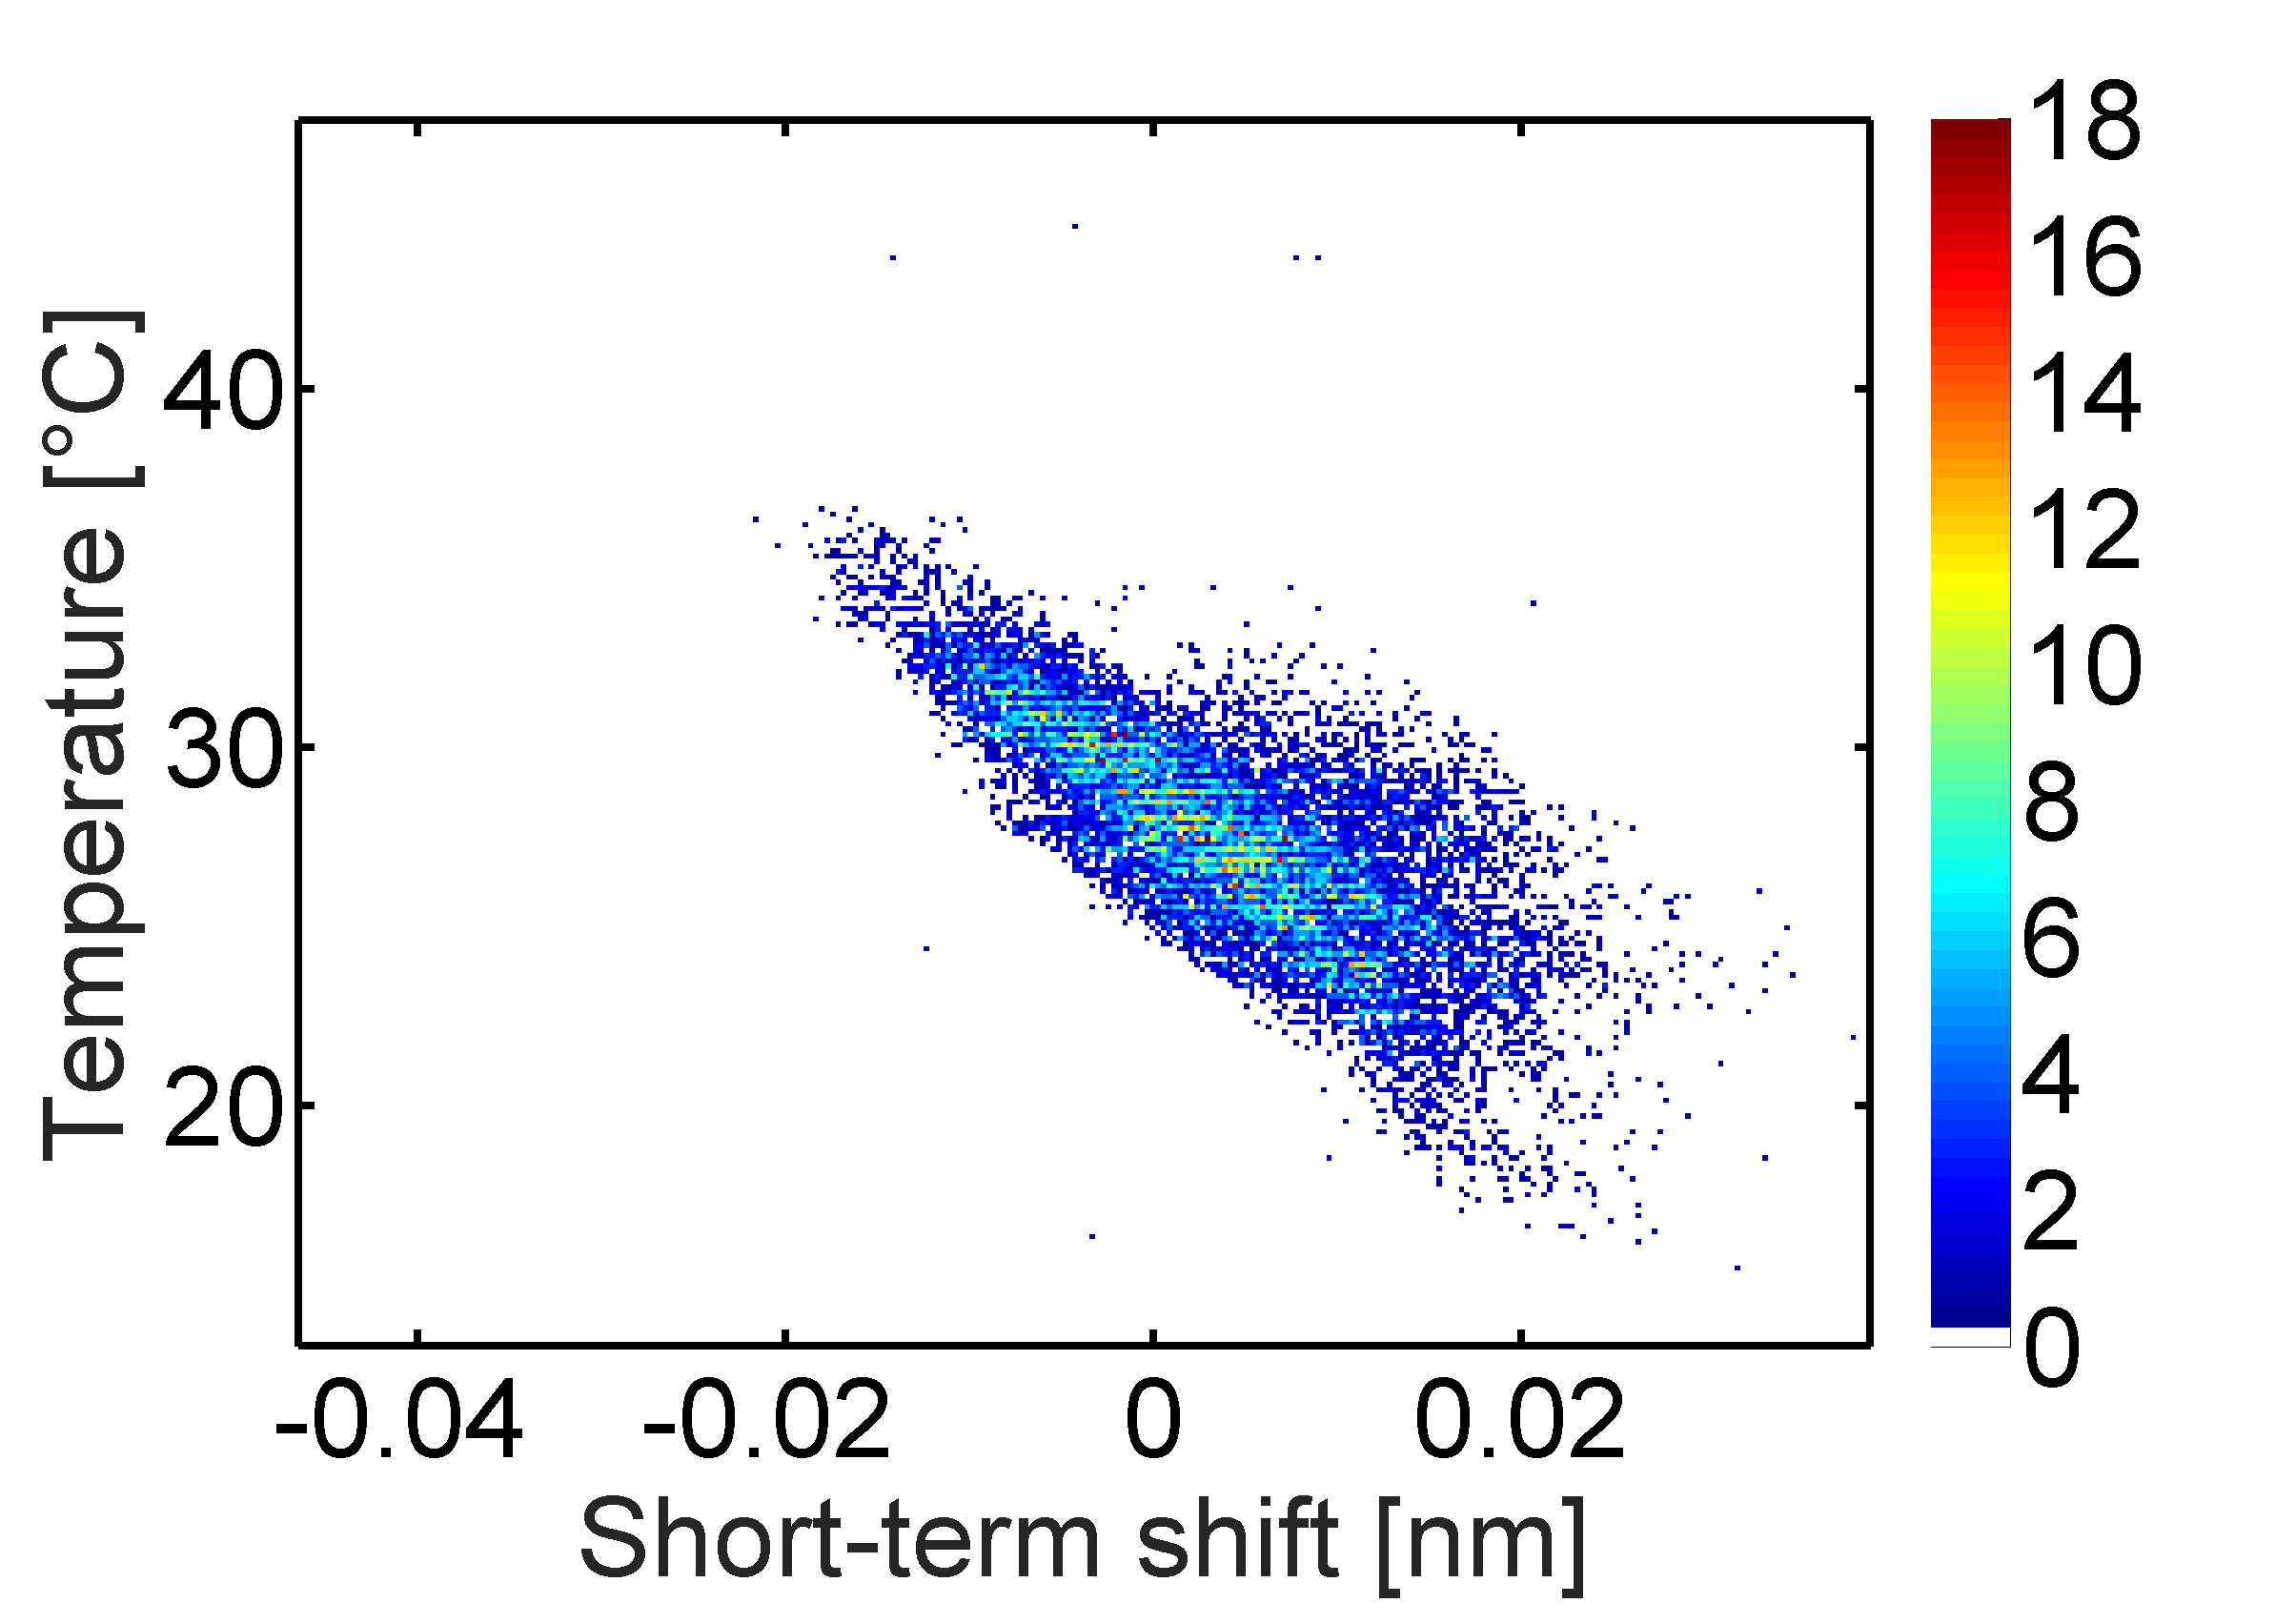
\includegraphics[width=0.49\textwidth]{Bilder/Simon/Bilder_Tung/D2J2140_After}}
		\caption{Titel unterm gesamten Bild}
		\label{fig:shorttermshift}
	\end{figure}
	\subsection{Temperature}
	The instrument design of the NOVAC instruments compromise between accuracy and longetivity as explained in \cref{NOVAC}. In particular there are no internal thermal stabilizations installed as an attempt to reduce the need for power. This can influence the recorded spectra.\\	
	Each pixel of the spectrometer, which is used for the DOAS experiment, collects photons of a certain wavelength range.\\
	The calibration for the wavelength to pixel mapping (WMP) is commonly done with a Mercury lamp or by the comparison with the high defined Kuruz spectrum.
	As the WMP depends on the optical alignment of the spectrometer, which itself depends on the temperature, it is not constant.
	Changes in the spectrometers temperature can cause changes in the instrument line function and shifts in the WMP (\cite{pinardi2007influence}). 
	Moreover, \cite{WarnachSimon} show that, short term shifts are related to the instrument temperature (see \Cref{fig:shorttermshift}).\\
	The above discussed temperature dependence of the WMP causes a reduction of the fitquality with increasing instrument temperature between plume and reference. Thus the \ce{BrO} Error increases as well with the temperature difference. To quantify the \ce{BrO} error dependency on the temperature all plume spectra of Tungurahua from August 2008 to August 2009 (Nevado del Ruiz from .... to ....) where evaluated with all plume spectra of the same time. In this time span 1647 "multi-add" spectra from tree different instruments where recorded, so we get approximately 1646$^2$ plume reference pairs and their corresponding \ce{BrO} error and temperature. The \ce{BrO} error as function of the temperature difference can be seen in \cref{fig:difftemp}. The blue dots shows the mean \ce{BrO} error at the specific temperature difference, the standard deviation is illustrated with gray bars.\\
	When compare the data of Tungurahua  and Nevado Del Ruiz it is noteworthy that the \ce{BrO} error on temperature dependence of the Data of Nevado Del Ruiz is stronger and the deviation is weaker than at Tungurahua, this may occur due to the larger temperature fluctuation at Nevado Del Ruiz. ?????????? quellen bitte!\\
	When looking at all discussed external parameters, temperature has  the strongest impact on the \ce{BrO} error due to the strong impact on the WMP.
	\begin{figure}[h!]			
		\subfigure[Data of Tungurahua]{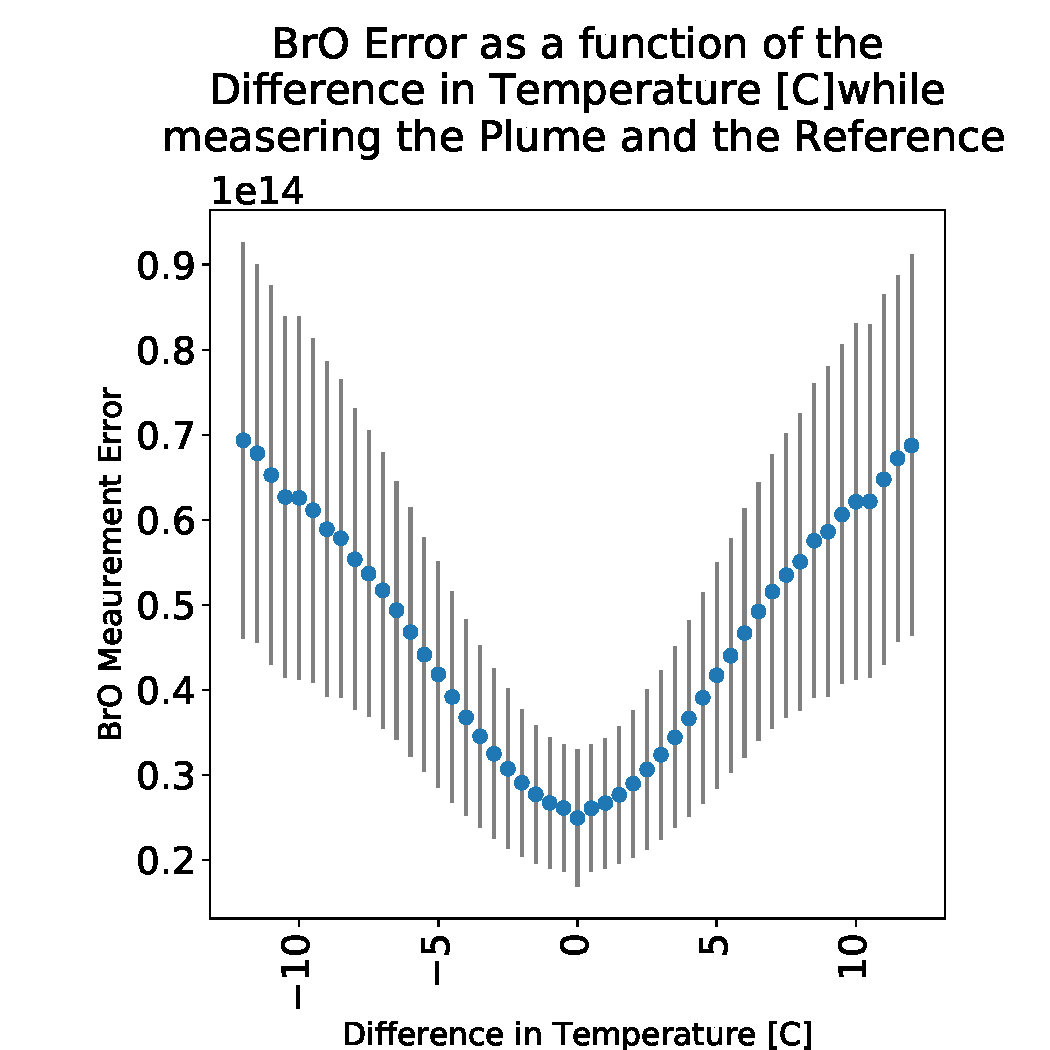
\includegraphics[width=0.49\textwidth]{Bilder/DiffTemp_Tungu}}
		\subfigure[Data of Nevado Del Riz]{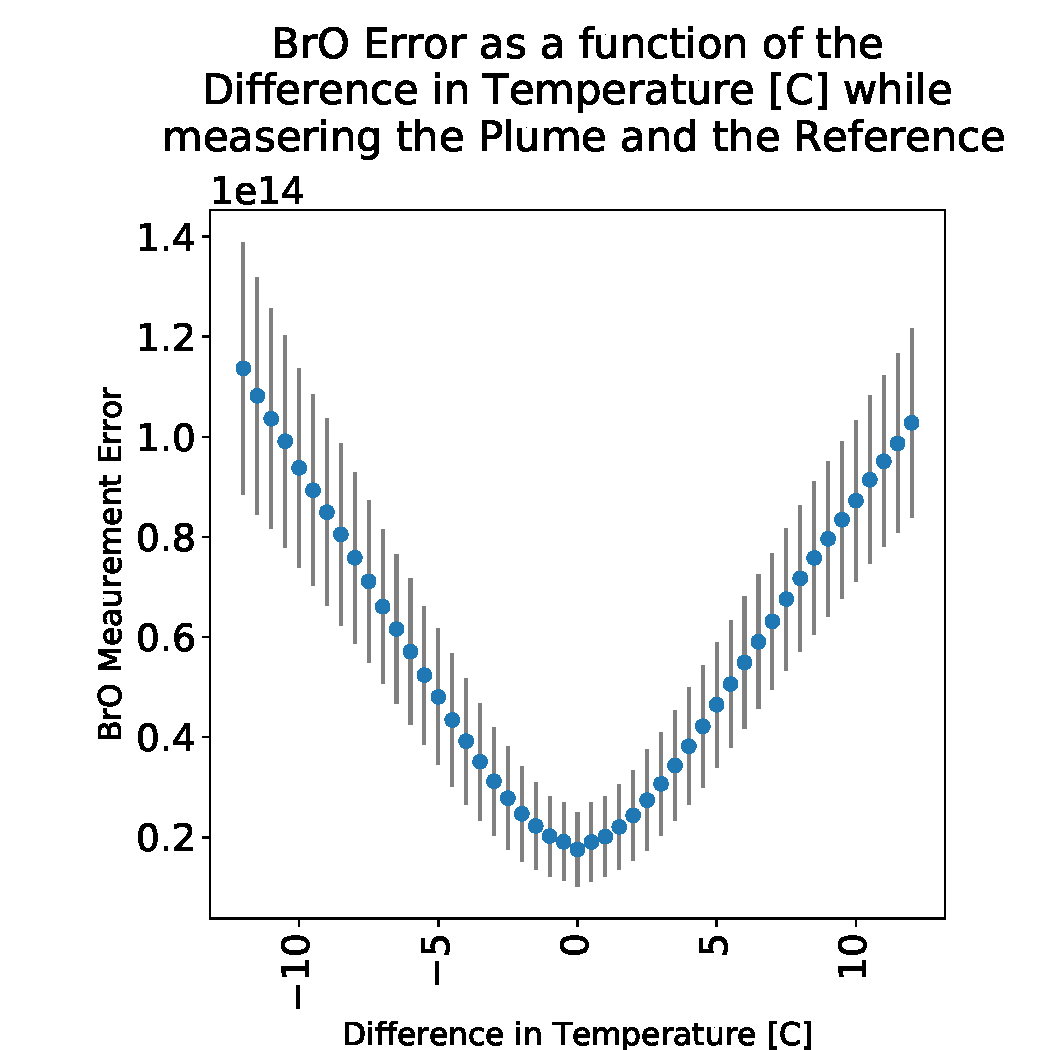
\includegraphics[width=0.49\textwidth]{Bilder/DiffTemp_Nevad}}
		\caption{The BrO Measurement Error as a function of the difference of temperature between measuring the reference and the plume are shown. To evaluate the plume spectra all reference spectra with a temporal distance of no longer than two weeks are used. A increase of the BrO Error with the distance in temperature is observable.}
		\label{fig:difftemp}
	\end{figure}[h!]
	\begin{itemize}
		\item The \ce{BrO} error has the strongest dependence on the temperature difference. At Tungurahua (Nevado Del Ruiz) the \ce{BrO} error increases by factor of $3.53\cdot10^{12}$  per degree.
		\begin{align*}
		\rightarrow&  BrO_{Error} = f(ext. P)+ 3.53\cdot10^{12}\cdot\frac{\Delta T}{1C^{\circ}} + \mathcal{O}\left(\right) & Tungurahua\\
		\rightarrow&  BrO_{Error} = f(ext. P)+7.56\cdot10^{12}\cdot\frac{\Delta T}{1C^{\circ}} + \mathcal{O}\left(\right) & Nevado Del Ruiz\\
		\end{align*}
	\end{itemize}
	\subsection{Daytime}
	During the day o al lot of external parameters like temperature, solar altitude etc. change. In particular the solar altitude could have an impact on the fit quality since the light path of the sun is much longer at the evening than at noon. \Cref{fig:diffdaytime} shows the dependency of the \ce{BrO} error on the daytime. The data are calculated as described for the temperature. As for the temperature the dependence of Nevado Del Ruiz is much larger than of Tungurahua, this might occur during the larger distance from the equator of Nevado Del Ruiz -> besser beschreiben

	\begin{figure}[h!]			
		
		\subfigure[Data of Tungurahua]{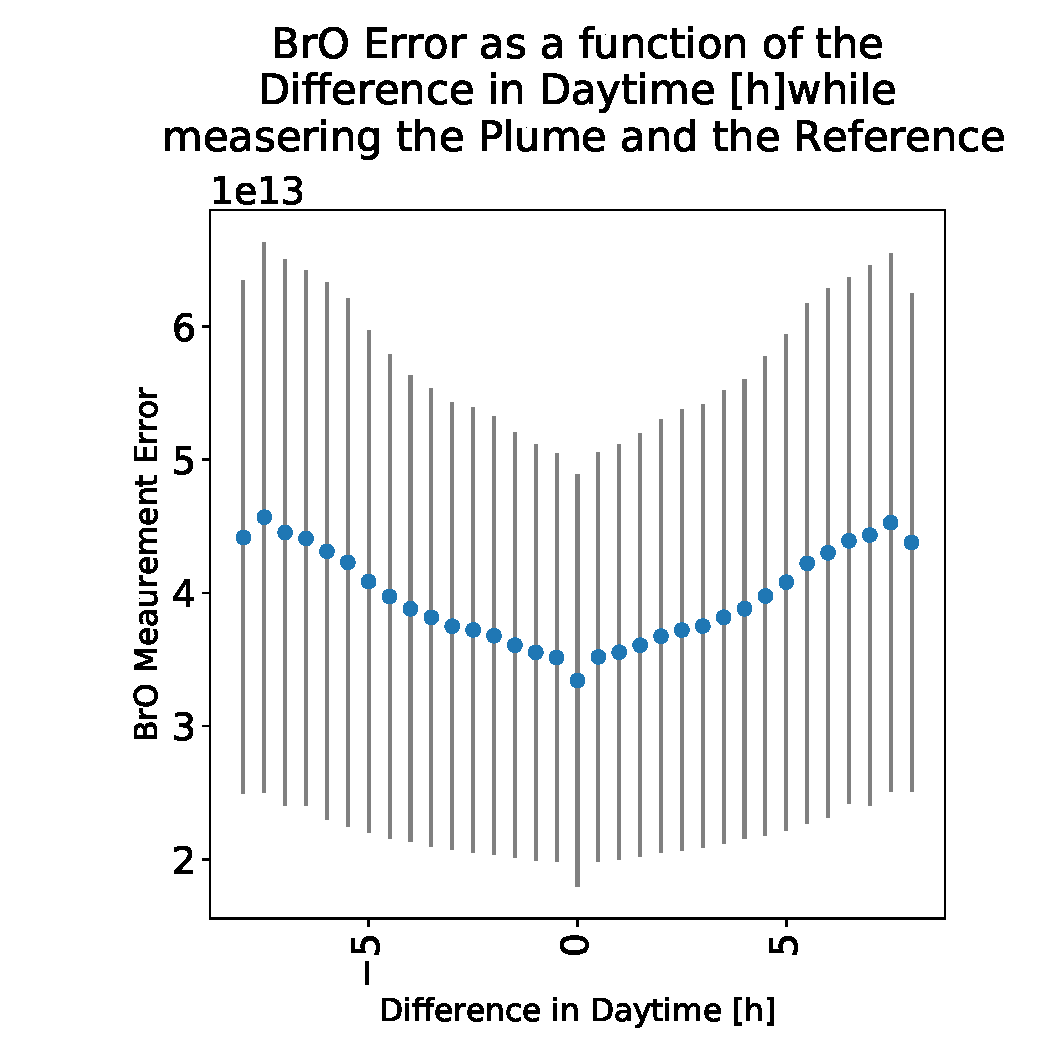
\includegraphics[width=0.49\textwidth]{Bilder/DiffDaytime_Tungu}}
		\subfigure[Data of Nevado Del Riz]{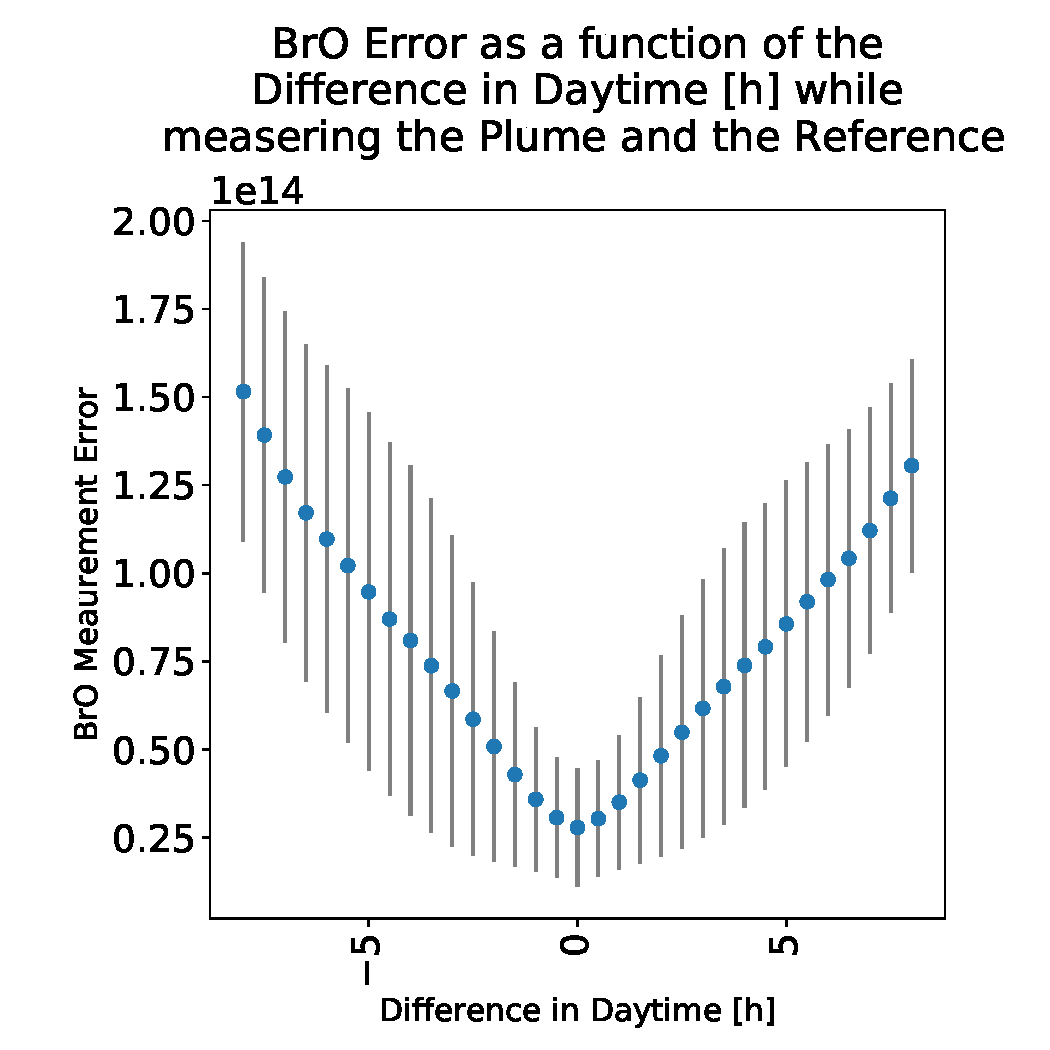
\includegraphics[width=0.49\textwidth]{Bilder/DiffDaytime_Nevad}}
		\caption{The BrO Measurement Error as a function of the difference of the day time between measuring the reference and the plume are shown. To evaluate the plume spectra all reference spectra with a temporal distance of no longer than two weeks are used. A increase of the BrO Error with the distance in day time is observable.}
		\label{fig:diffdaytime}
	\end{figure}
	\begin{itemize}
		\item We found a dependency of the \ce{BrO} error on the daytime. We assume, that this dependency comes from other external parameters which change during the day. 
		\item The \ce{BrO} Error increases with the daytime differences like: \\
		\begin{align*}
		\rightarrow&  BrO_{Error} = f(ext. P)+1.33\cdot10^{12}\cdot\frac{\Delta DT}{1h}  + \mathcal{O}\left(\right)& Tungurahua\\
		\rightarrow&  BrO_{Error} = f(ext. P)+1.58\cdot10^{13}\cdot\frac{\Delta DT}{1h} + \mathcal{O}\left(\right) & Nevado Del Ruiz\\
		\end{align*}
		
	\end{itemize}
	\subsection{Colorindex}
	\begin{figure}[h]		
		\subfigure[Data of Tungurahua]{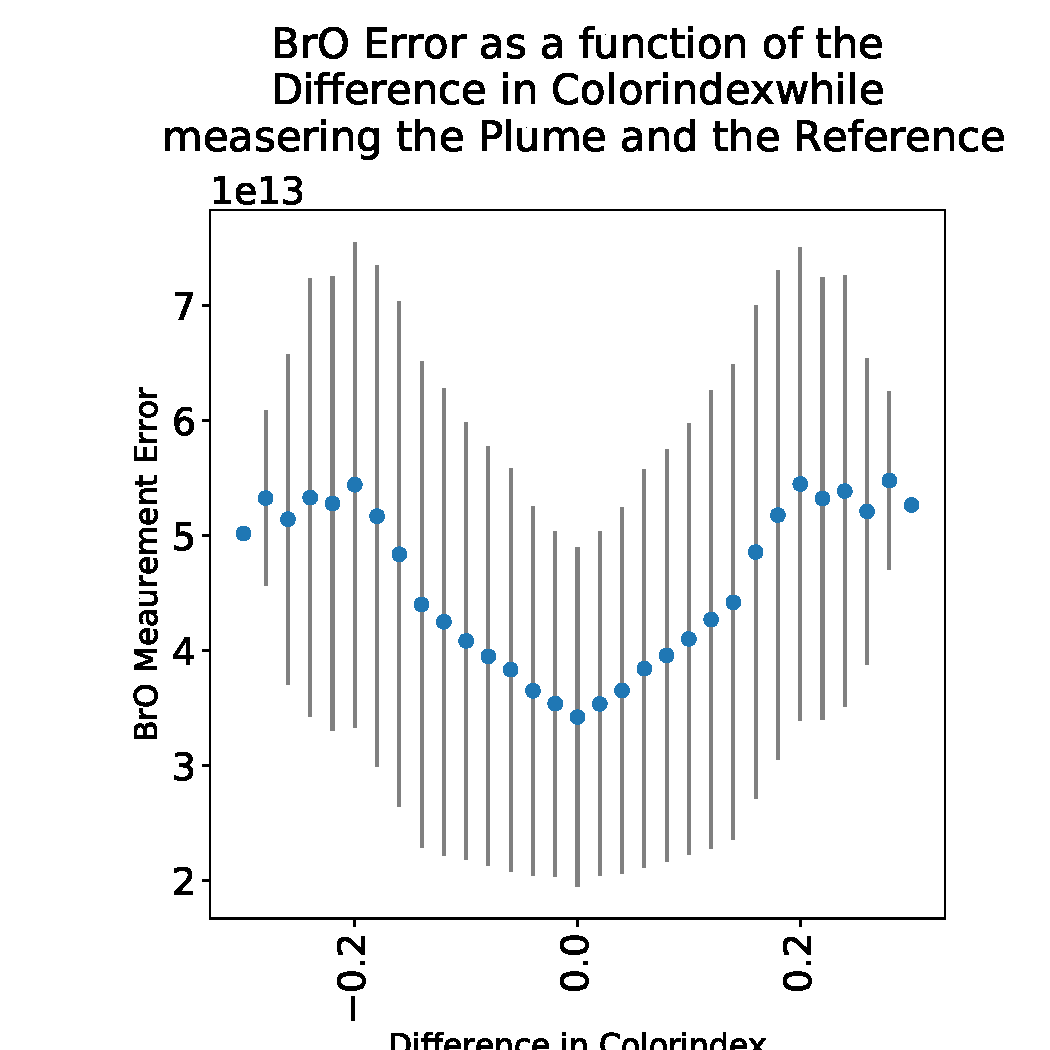
\includegraphics[width=0.49\textwidth]{Bilder/DiffColidx_Tungu}}
		\subfigure[Data of Nevado Del Riz]{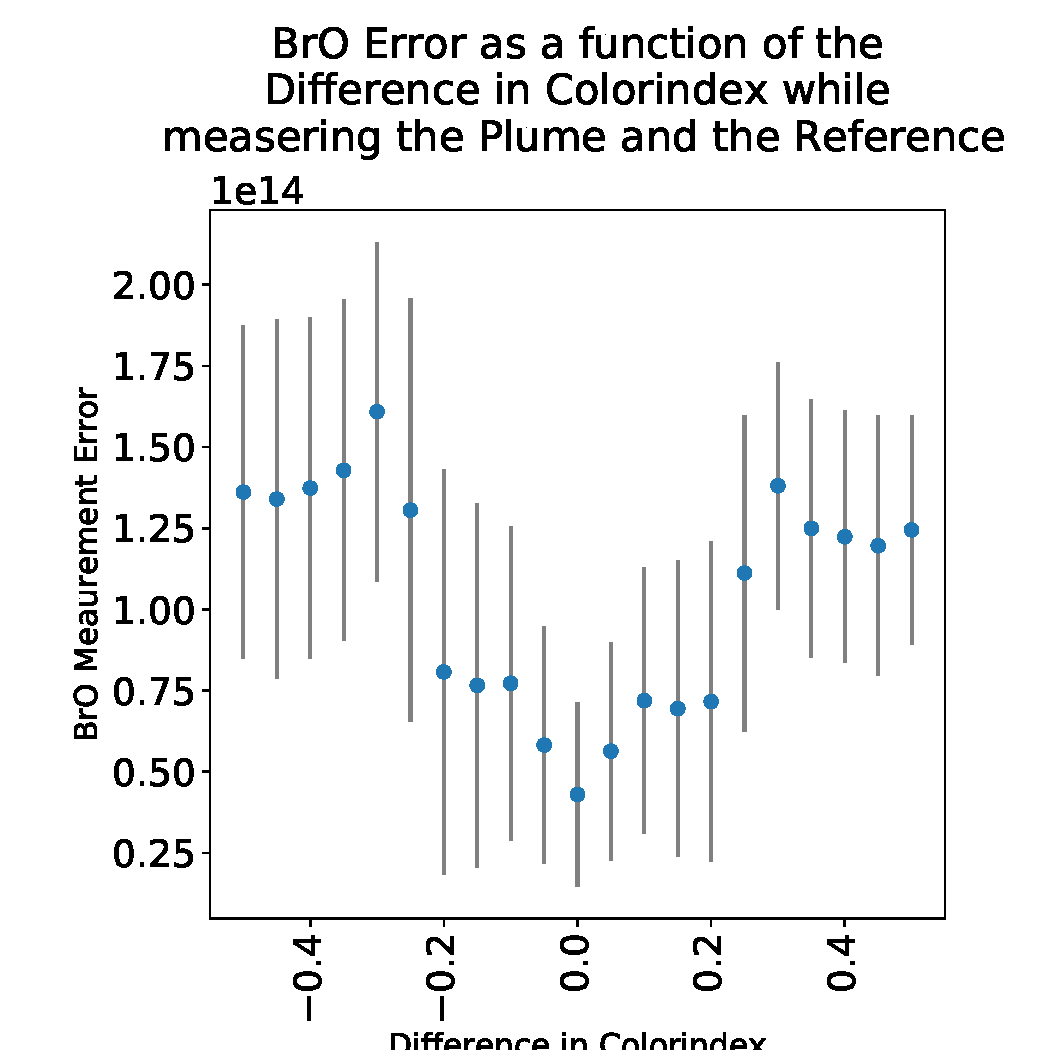
\includegraphics[width=0.49\textwidth]{Bilder/DiffColidx_Nevad}}
		\caption{The BrO Measurement Error as a function of the difference of colorindex between measuring the reference and the plume are shown. To evaluate the plume spectra all reference spectra with a temporal distance of no longer than two weeks are used. A increase of the BrO Error with the distance in colorindex is observably.}
		\label{fig:diffcolidx}
	\end{figure}
	Clouds  have  a  strong  influence  on  the  atmospheric  radiative  transfer  and  thus  affect  the  interpretation  and  analysis of DOAS - observations \cite{wagner2014cloud}.
	
	Clouds can be identified by several measurement quantities that they influence.
	As Mie scattering is dominant in clouds the wavelength of the light that is scattered is different than the Rayleigh sky. Thus, clouds can be easily identified by their white color.
	Therefore, the cloudiness of the sky can be quantified in a scalar measure defined by the ratio of the measured intensity at two wavelengths, the so-called colour index.
	\cite{wagner2014cloud} showed that for a zenith-looking instrument the measured radiation intensity is enhanced by clouds. Thus, clouds can cause large errors for the retrieved gas column density and the corresponding uncertainties. 
	Cloud effects are especially severe if the cloudiness for the recorded plume and reference spectra strongly defer. Also for broken clouds the described effect can be observed as measurements at some elevation angles might be influenced by clouds while others are not.
	In this work the Colour Index (CI) is the ratio between the intensities at 320nm and 360 nm.
	These two wavelengths are as far apart as the filter used for stray-light prevention in the spectrometers allows.
	%% I don’t understand 	
	On the other hand, the lower wavelength avoids the deep UV range where \ce{SO2} and O3 absorption plays a dominant role.
	%% I don’t understand 	
	The Mie scattering in the clouds is responsible for the higher amount of radiation from larger wavelengths. This results in a decrease of the CI (\cite{lubcke2014optical}).
	\\
	We evaluated the CI at the zenith, to increase the stability of the fit we added in each cases 10 intensitys. Using always the zenith to evaluate the colour index makes the colour index more comparable, but if broken clouds occur, the CI of the reference and the plume could differ from the calculated CI of the zenith. This could be a reason for the large deviations of the mean \ce{BrO} error as function of the colour index (see \cref{fig:diffcolidx})

	\begin{itemize}
		\item 	The \ce{BrO} Error increases with the Colorindex differences as \\
		\begin{align*}
		\rightarrow&  BrO_{Error} = f(ext. P)+ 1.01\cdot10^{13}\cdot\frac{\Delta Cidx}{0.1} + \mathcal{O}\left(\right) & Tungurahua\\
		\rightarrow&  BrO_{Error} = f(ext. P)+  4\cdot10^{13}\cdot\frac{\Delta Cidx}{0.1} + \mathcal{O}\left(\right) & Nevado Del Ruiz\\
		\end{align*}
	\end{itemize}
	\subsection{Elevation Angle}
		\begin{figure}[h!]			
		\subfigure[Data of Tungurahua]{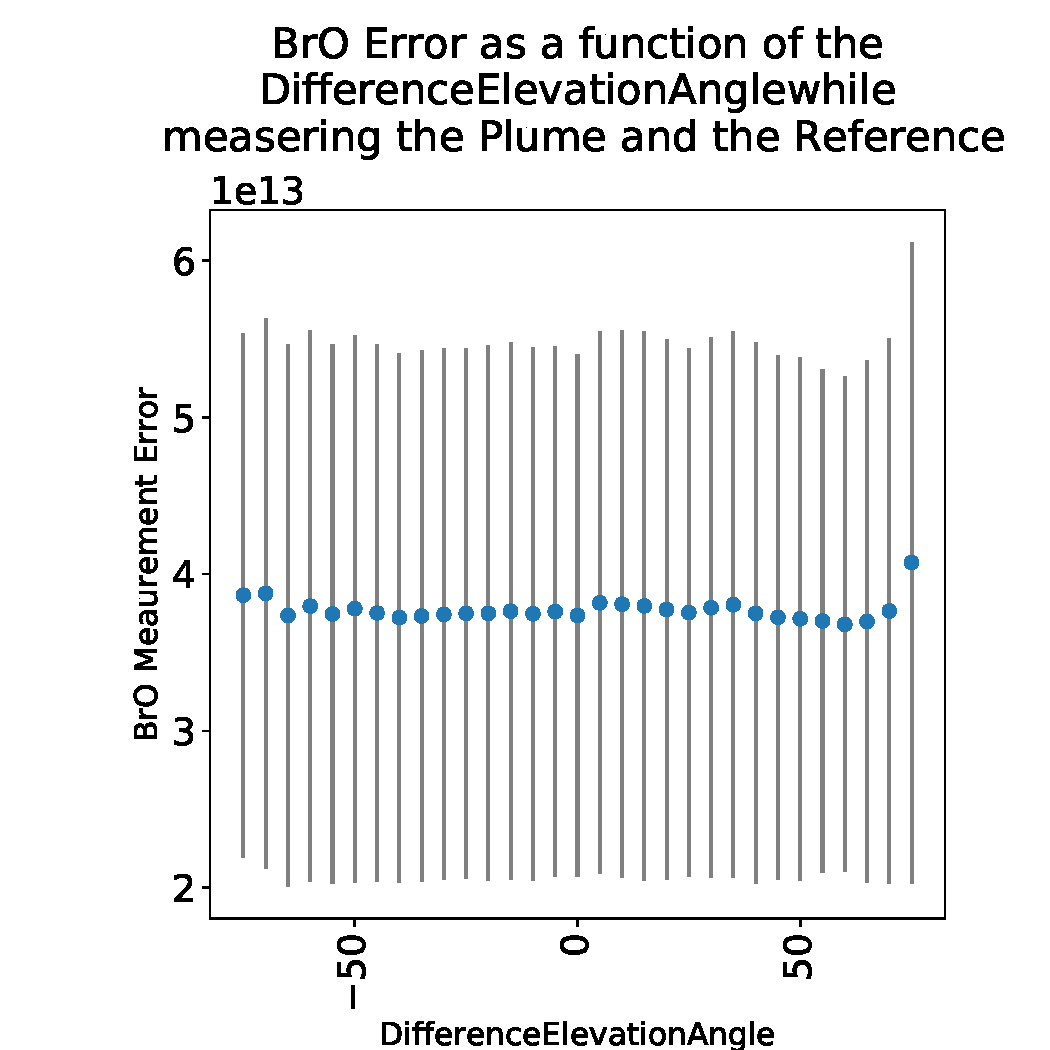
\includegraphics[width=0.49\textwidth]{Bilder/DiffElevAngle_Tungu}}
		\subfigure[Data of Nevado Del Riz]{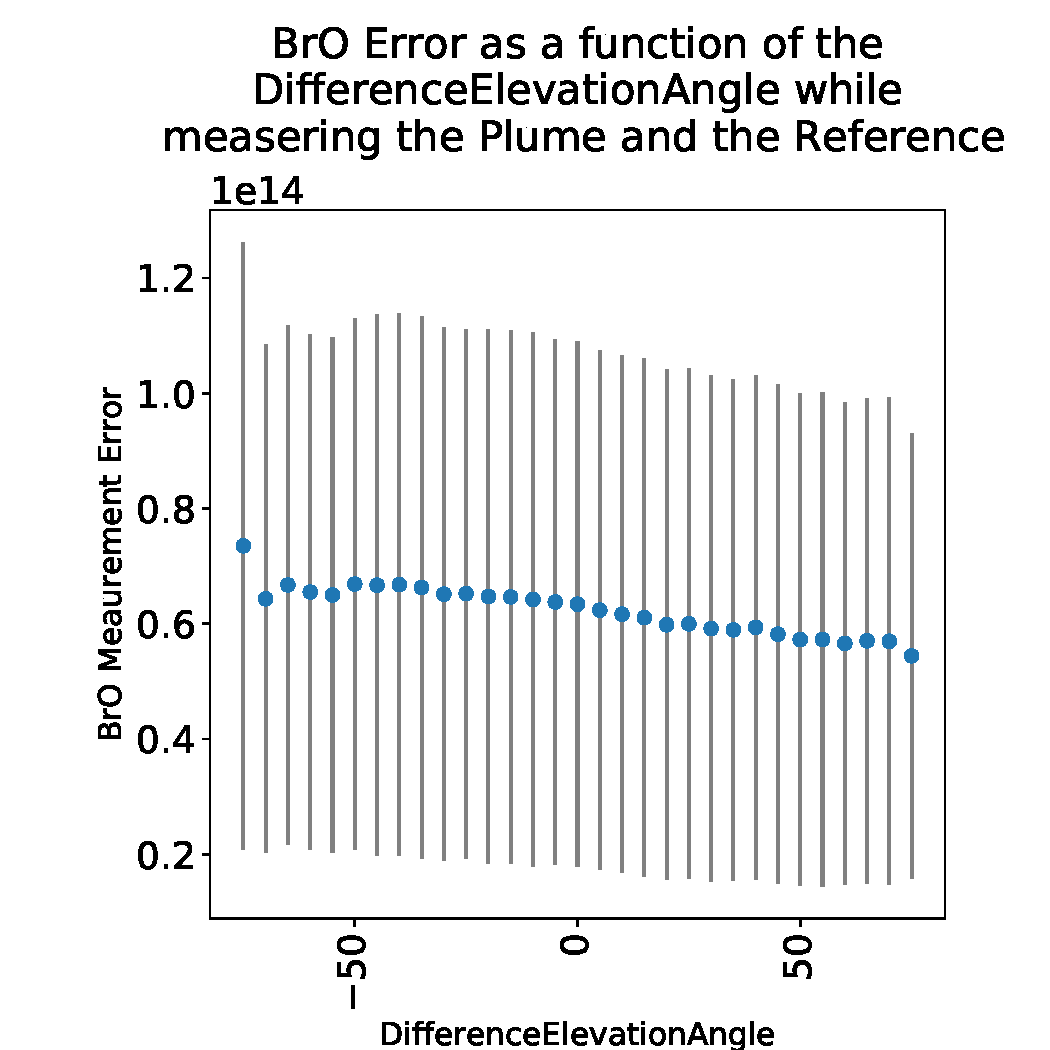
\includegraphics[width=0.49\textwidth]{Bilder/DiffElevAngle_Nevad}}
		\caption{The BrO Measurement Error as a function of the Elevation Angle. To evaluate the plume spectra all reference spectra with a temporal distance of no longer than two weeks are used. We can't see any significant correlation.}
	\end{figure}
	The elevation angle describes the angle between the horizon and the zenith. When using the plume spectrum and the reference spectrum of the same time, the difference in elevation angle cannot be zero, since the plume is always somewhere else than the reference located.\\
	The \ce{BrO} error doesn't depend significantly on the difference between the Elevation Angles. This could have several reasons. One problem is, that the Elevation Angle of Plume and Reference spectrum is not the same. This could also be a reason of uncertainty of the evaluations of the plume spectrum.




	\subsection{Exposure Time}
	\begin{figure}		
		\subfigure[Data of Tungurahua]{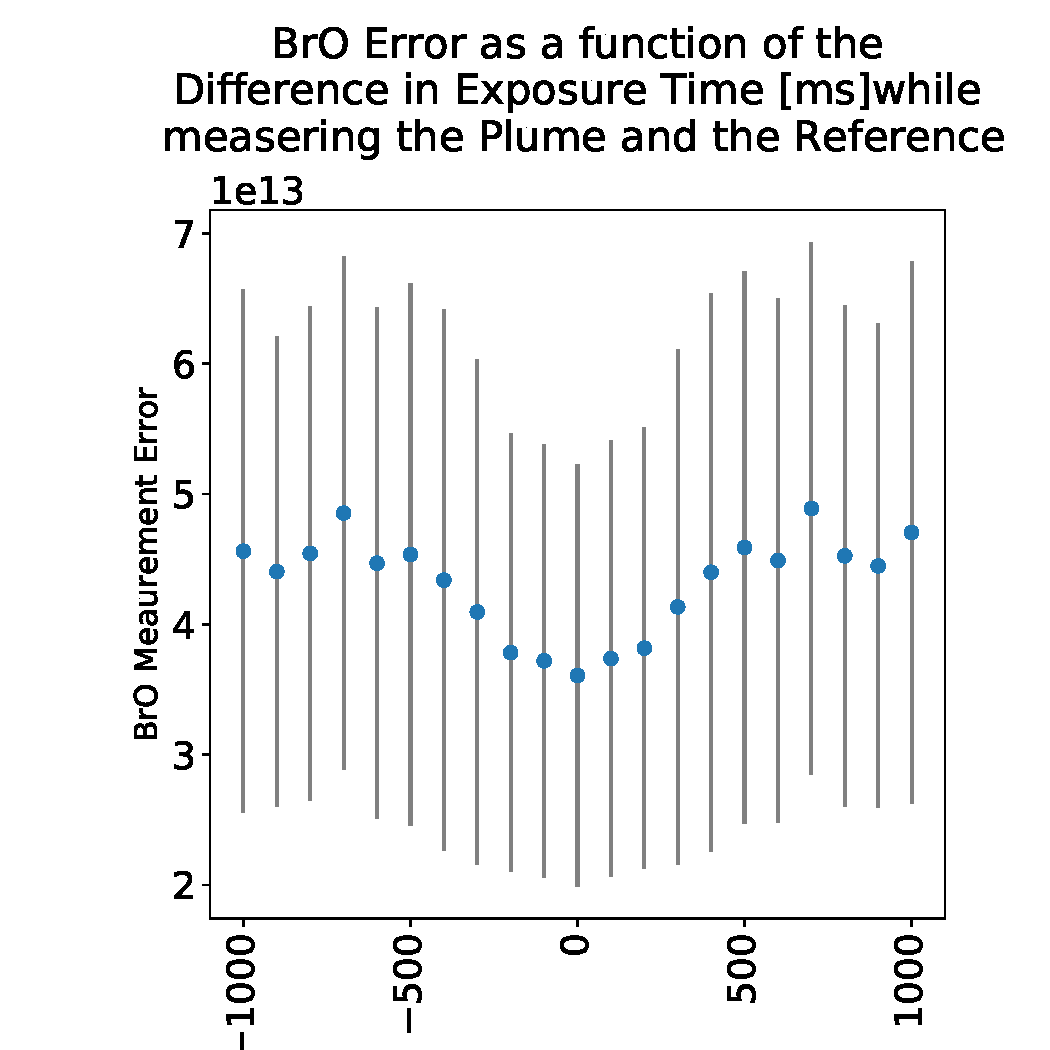
\includegraphics[width=0.49\textwidth]{Bilder/DiffExpTime_Tungu}}
		\subfigure[Data of Nevado Del Riz]{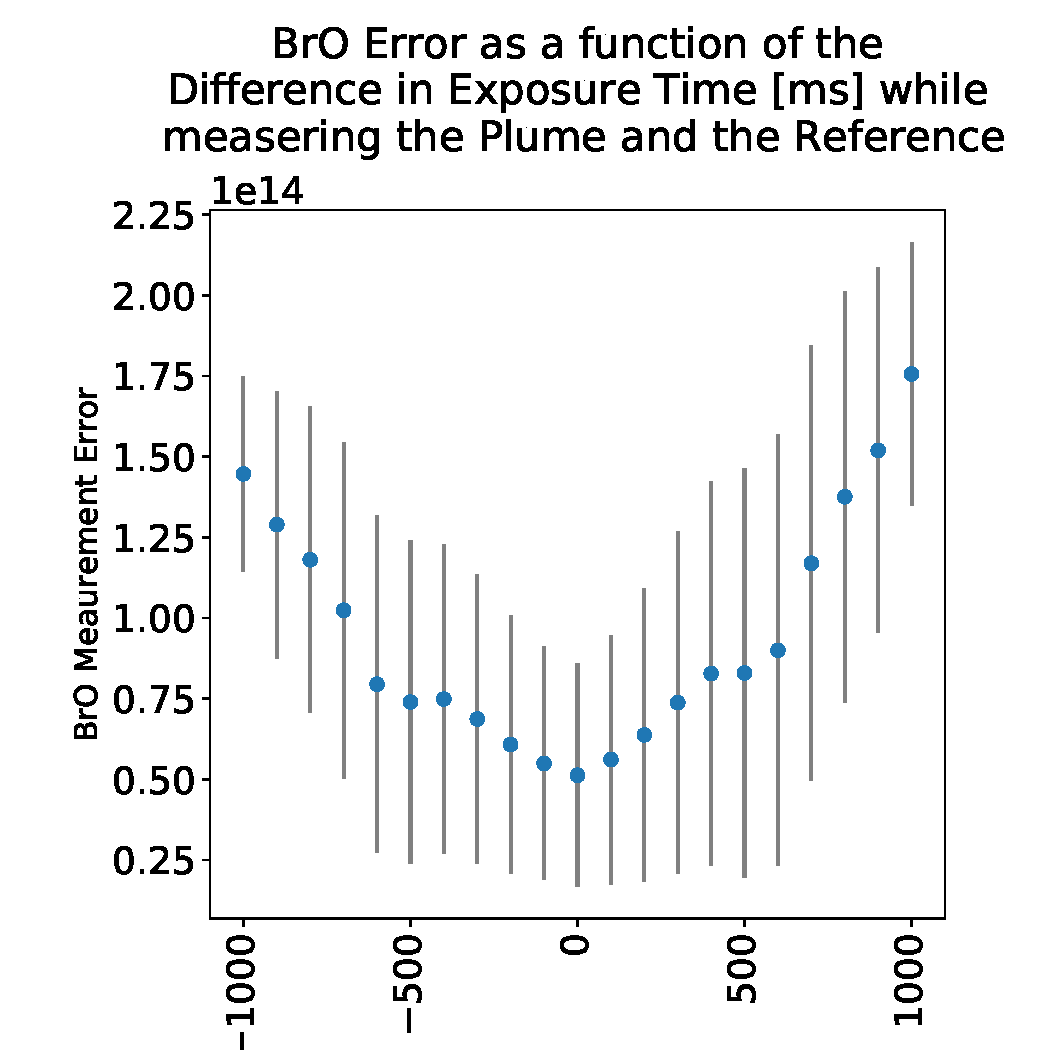
\includegraphics[width=0.49\textwidth]{Bilder/DiffExpTime_Nevad}}
		\caption{The BrO Measurement Error as a function of the difference of exposure time between measuring the reference and the plume are shown. To evaluate the plume spectra all reference spectra with a temporal distance of no longer than two weeks are used. A increase of the BrO Error with the distance in exposure time is observably.}
		\label{fig:diffexptime}
	\end{figure}
	The Exposure Time is a degree of sky lightness.The  exposure time is the length of time the sensor of the NOVAC instrument is exposed to light. The amount of light that reaches the film or image sensor is proportional to the exposure time. The exposure time is adjusted in the way that the maximum intensity does not overly the capacity of the sensor.\\
	We can observe an small dependency of the \ce{BrO} error on the Exposure time at Tungurahua and Nevado Del Ruiz as it is shown in \cref{fig:diffexptime}
	

	\begin{itemize}
		\item The \ce{BrO} Error increases with the exposure time differences as\\
		\begin{align*}
		\rightarrow&  BrO_{Error} = f(ext. P)+ 1.92\cdot10^{12}\cdot\frac{\Delta ET}{10^{-2}s} + \mathcal{O}\left(\right) & Tungurahua\\
		\rightarrow&  BrO_{Error} = f(ext. P)+ 1.0\cdot10^{13}\cdot\frac{\Delta T}{10^{-2}s} + \mathcal{O}\left(\right) & Nevado Del Ruiz\\
		\end{align*}
	\end{itemize}
	\subsection*{Dependency of external parameters on each other}
		\textbf{Difference of Temperature on  Difference of Exposure Time}
		\begin{equation}
		\Delta T =  -26.32\cdot \Delta ExpTime + 2\cdot 10^{-15}
		\end{equation}
		
		\textbf{Difference of Temperature on  Difference of colorindex}
		\begin{equation}
		\Delta T = 0.0022\cdot \Delta ColIdX +2\cdot 10^{-19}
		\end{equation}
		
				\textbf{Difference of Temperature on  Difference of Day time}
		\begin{equation}
		\Delta T =0.262\cdot \Delta daytime -4\cdot 10^{-17}
		\end{equation}
		
						\textbf{Difference of Temperature on  Difference of Elevation angle}
		\begin{equation}
		\Delta T =1.08\cdot \Delta Elev Angle -1\cdot 10^{-16}
		\end{equation}

		\textbf{Difference of Exposure on  Difference of  Col Idx}
		\begin{equation}
		\Delta Exposure  =-6.22\cdot 10^{-5} \Delta Col Idx  +1\cdot 10^{-18}
		\end{equation}
		
				\textbf{Difference of  Exposure on  Difference of Day time}
		\begin{equation}
		\Delta Exposure  =-0.004\cdot \Delta daytime -1\cdot 10^{-17}
		\end{equation}
		
						\textbf{Difference of  Exposure  on  Difference ofElevation angle}
		\begin{equation}
		\Delta Exposure  =-0.047\cdot \Delta  ElevAngle +3\cdot 10^{-16}
		\end{equation}


		\textbf{Difference of  Colorindex  on  Difference of Day time}
		\begin{equation}
		\Delta ColIdX  =4.51\cdot \Delta daytime-1.2\cdot 10^{-15}
		\end{equation}
		
		\textbf{Difference of  Colorindex  on  Difference of Elevation angle}
		\begin{equation}
		\Delta ColIdX  =-52\cdot \Delta ElevAngle+ 1.45\cdot 10^{-14}
		\end{equation}
		
				\textbf{Difference of  Colorindex  on  Difference of Elevation angle}
		\begin{equation}
		\Delta ColIdX  =3.5\cdot \Delta ElevAngle-6\cdot 10^{-16}
		\end{equation}
	\begin{figure}
			\subfigure[I2J8546\_0]{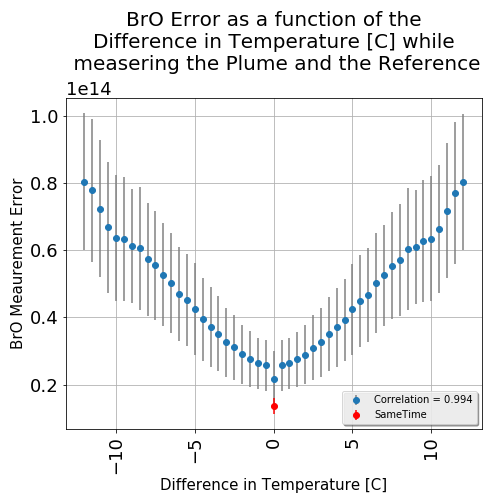
\includegraphics[width=0.3\linewidth]{Bilder/BrOError_onVariables_050218/I2J8546_0DiffTemp_Tungu}}
			\subfigure[I2J8548\_0]{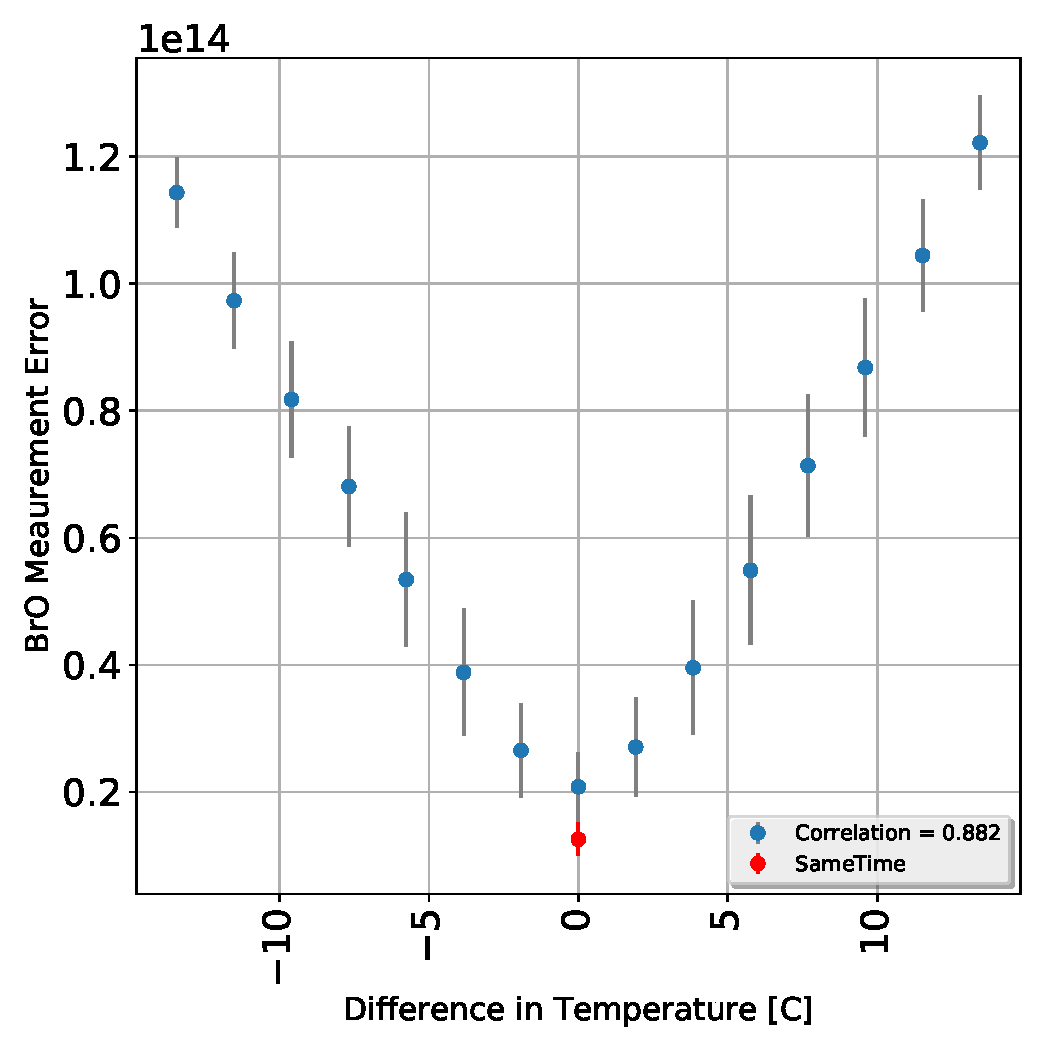
\includegraphics[width=0.3\linewidth]{Bilder/BrOError_onVariables_050218/I2J8548_0DiffTemp_Tungu}}
			\subfigure[D2J2140\_0]{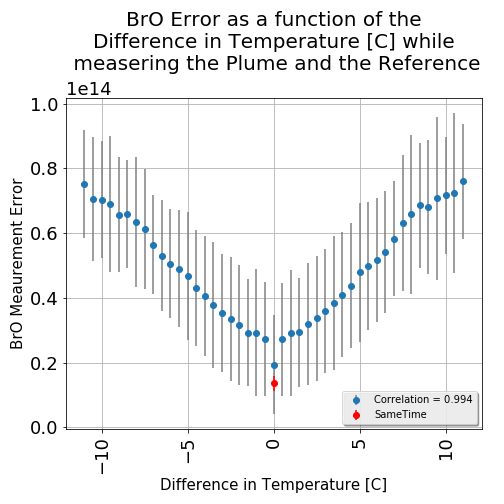
\includegraphics[width=0.3\linewidth]{Bilder/BrOError_onVariables_050218/D2J2140_0DiffTemp_Tungu}}
			\caption{DiffTemp at Tungurahua}
			\label{fig:DiffTemptunge}
	\end{figure}
	\begin{figure}
		\subfigure[I2J8546\_0]{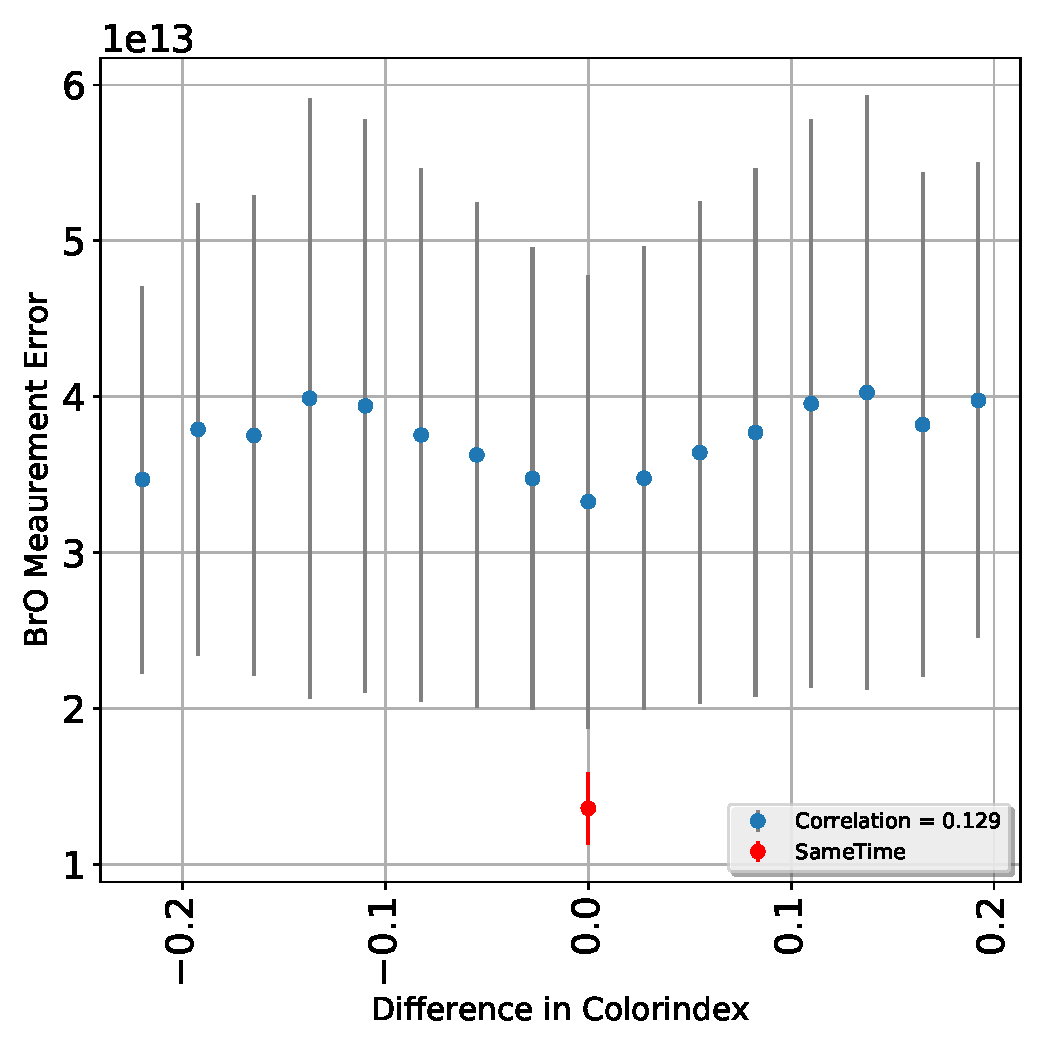
\includegraphics[width=0.3\linewidth]{Bilder/BrOError_onVariables_050218/I2J8546_0DiffColidx_Tungu}}
		\subfigure[I2J8548\_0]{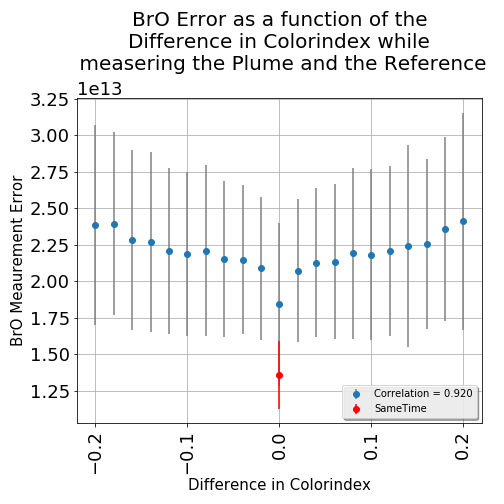
\includegraphics[width=0.3\linewidth]{Bilder/BrOError_onVariables_050218/I2J8548_0DiffColidx_Tungu}}
		\subfigure[D2J2140\_0]{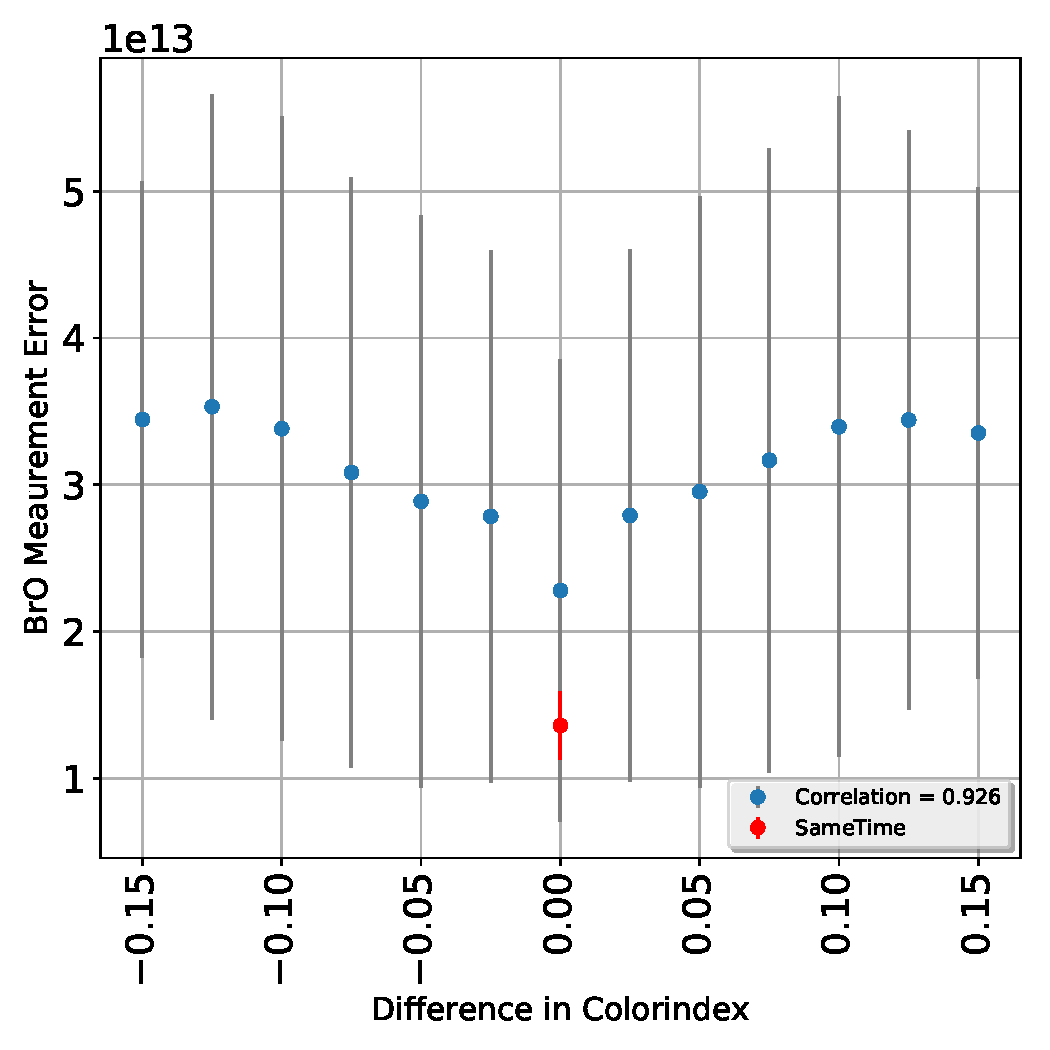
\includegraphics[width=0.3\linewidth]{Bilder/BrOError_onVariables_050218/D2J2140_0DiffColidx_Tungu}}
		\caption{Colorindex at Tungurahua}
		\label{fig:diffcolidxtungu}
	\end{figure}
	\begin{figure}
		\subfigure[I2J8546\_0]{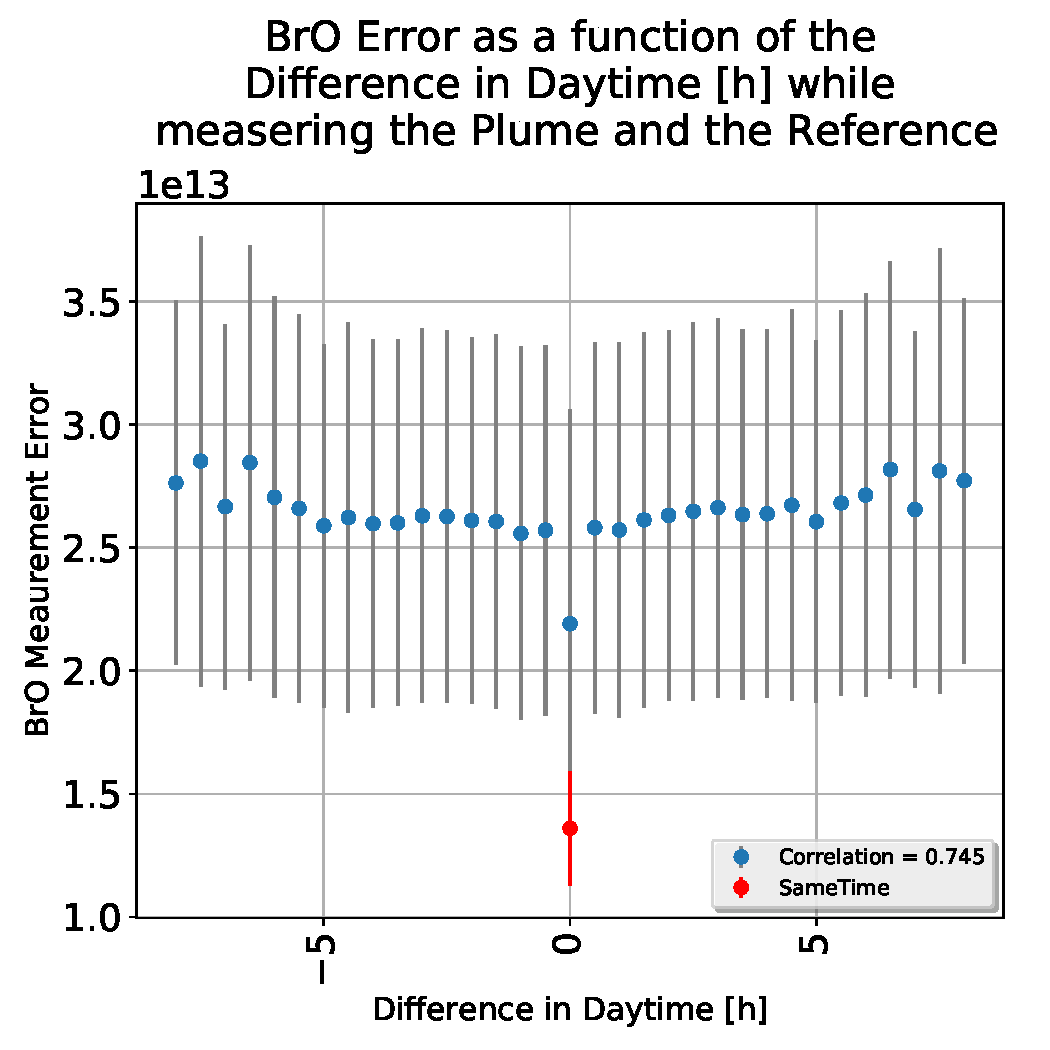
\includegraphics[width=0.3\linewidth]{Bilder/BrOError_onVariables_050218/I2J8546_0DiffDaytime_Tungu}}
		\subfigure[I2J8548\_0]{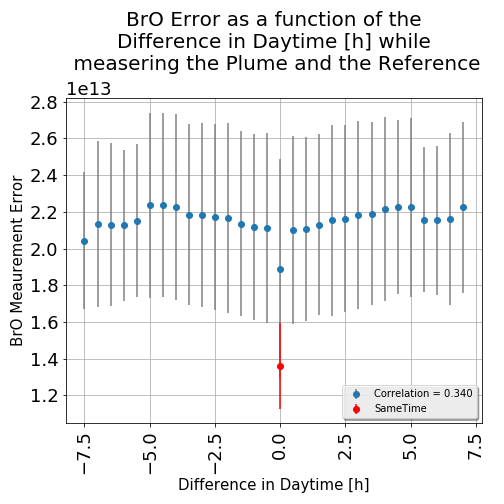
\includegraphics[width=0.3\linewidth]{Bilder/BrOError_onVariables_050218/I2J8548_0DiffDaytime_Tungu}}
		\subfigure[D2J2140\_0]{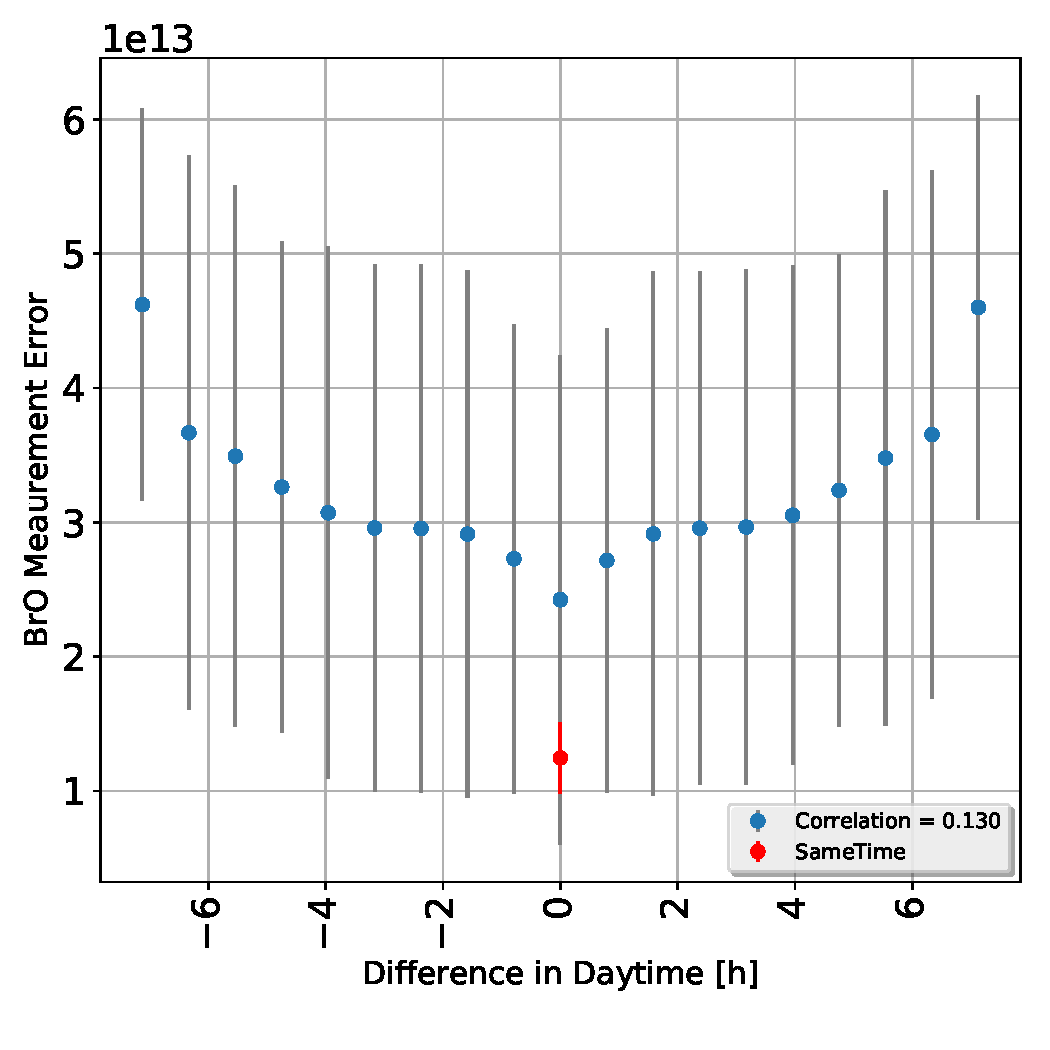
\includegraphics[width=0.3\linewidth]{Bilder/BrOError_onVariables_050218/D2J2140_0DiffDaytime_Tungu}}
		\caption{Colorindex at Tungurahua}
		\label{fig:DiffDaytime}
	\end{figure}
	\begin{figure}
		\subfigure[I2J8546\_0]{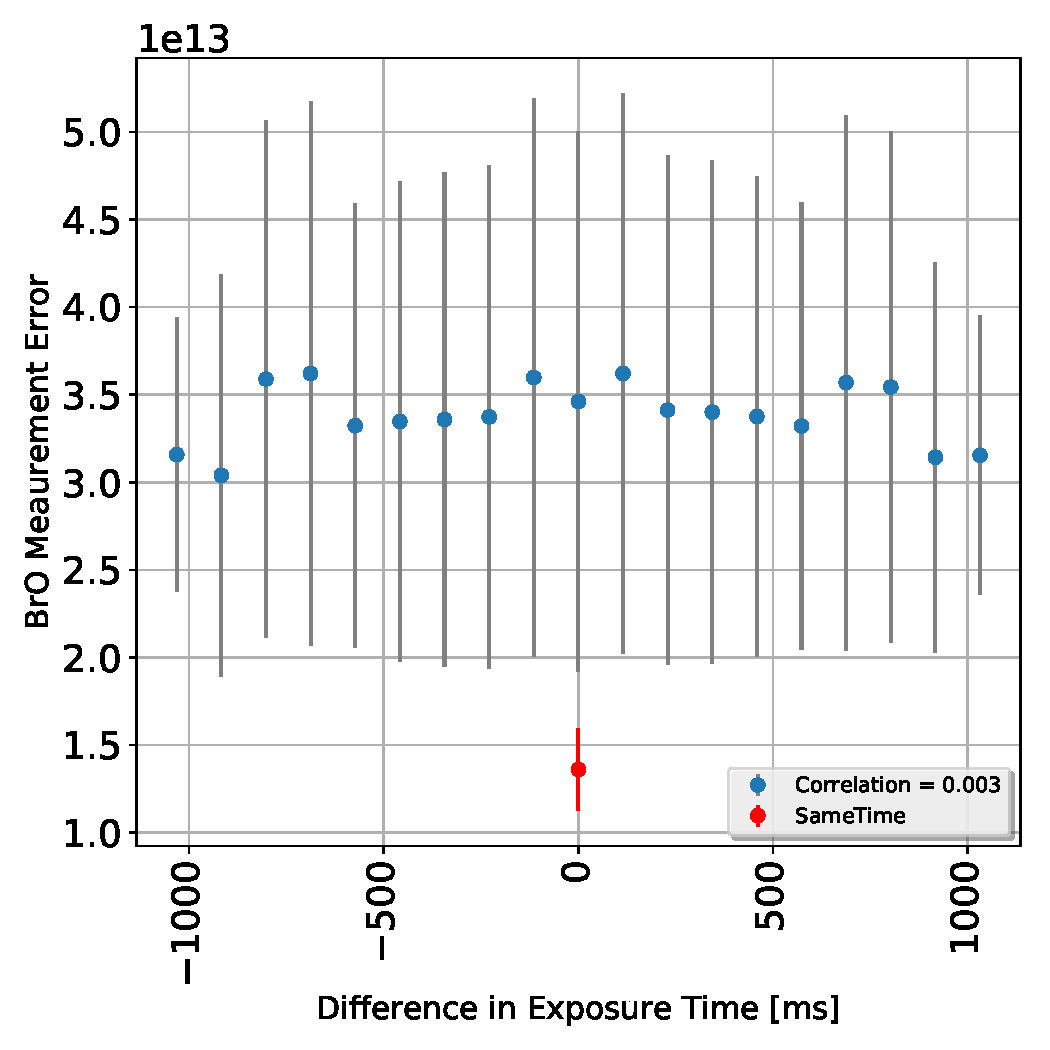
\includegraphics[width=0.3\linewidth]{Bilder/BrOError_onVariables_050218/I2J8546_0DiffExpTime_Tungu}}
		\subfigure[I2J8548\_0]{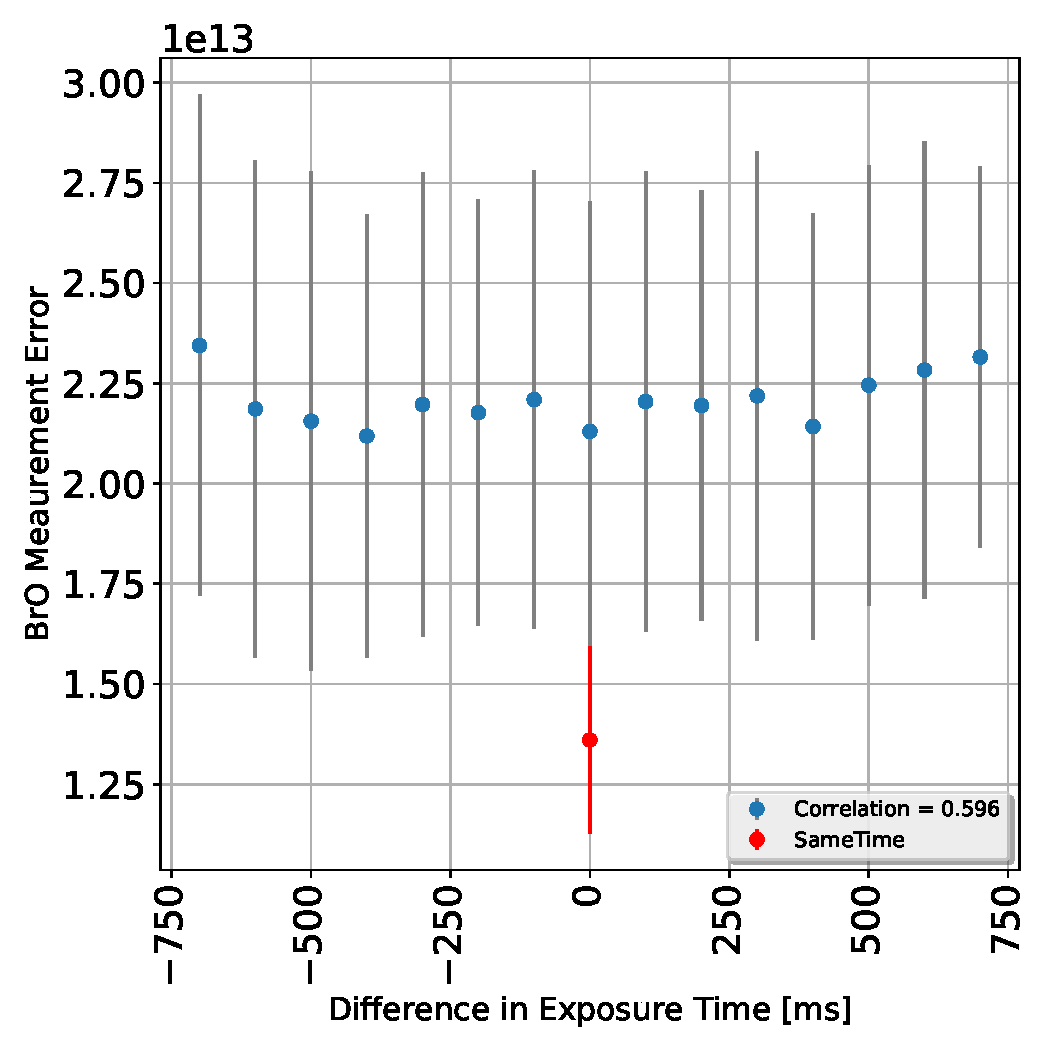
\includegraphics[width=0.3\linewidth]{Bilder/BrOError_onVariables_050218/I2J8548_0DiffExpTime_Tungu}}
		\subfigure[D2J2140\_0]{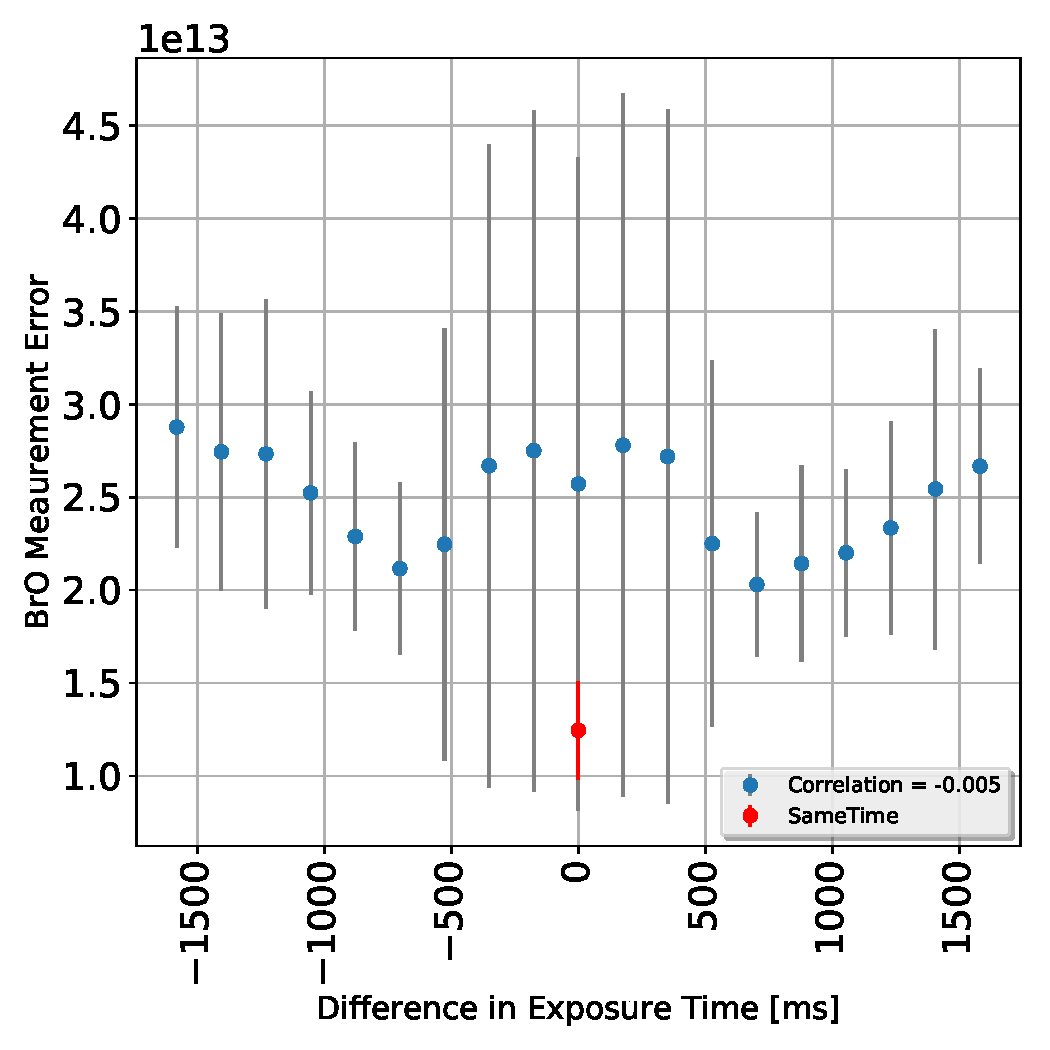
\includegraphics[width=0.3\linewidth]{Bilder/BrOError_onVariables_050218/D2J2140_0DiffExpTime_Tungu}}
		\caption{DiffExpTime at Tungurahua}
		\label{fig:DiffExpTime}
	\end{figure}
	
	%--------------------------------------------------------------------------------------------------------------
	\chapter{Method}
	Based on the findings about the influence of external parameters on the \ce{BrO} error we developed an algorithm which is able to pick an appropriate volcanic-trace-gas free reference.\\ 
	The first step is, to evaluate every reference with solar atlas spectrum, to check for contamination.	A Spectrum is treated as contaminated if the \ce{SO2} column density of the reference (evaluated with a solar atlas spectrum) is larger as 2$\cdot 10^{17}\frac{molec}{cm^2}$.\\
	\\
	If the reference is contaminated:
	\begin{figure}
\centering
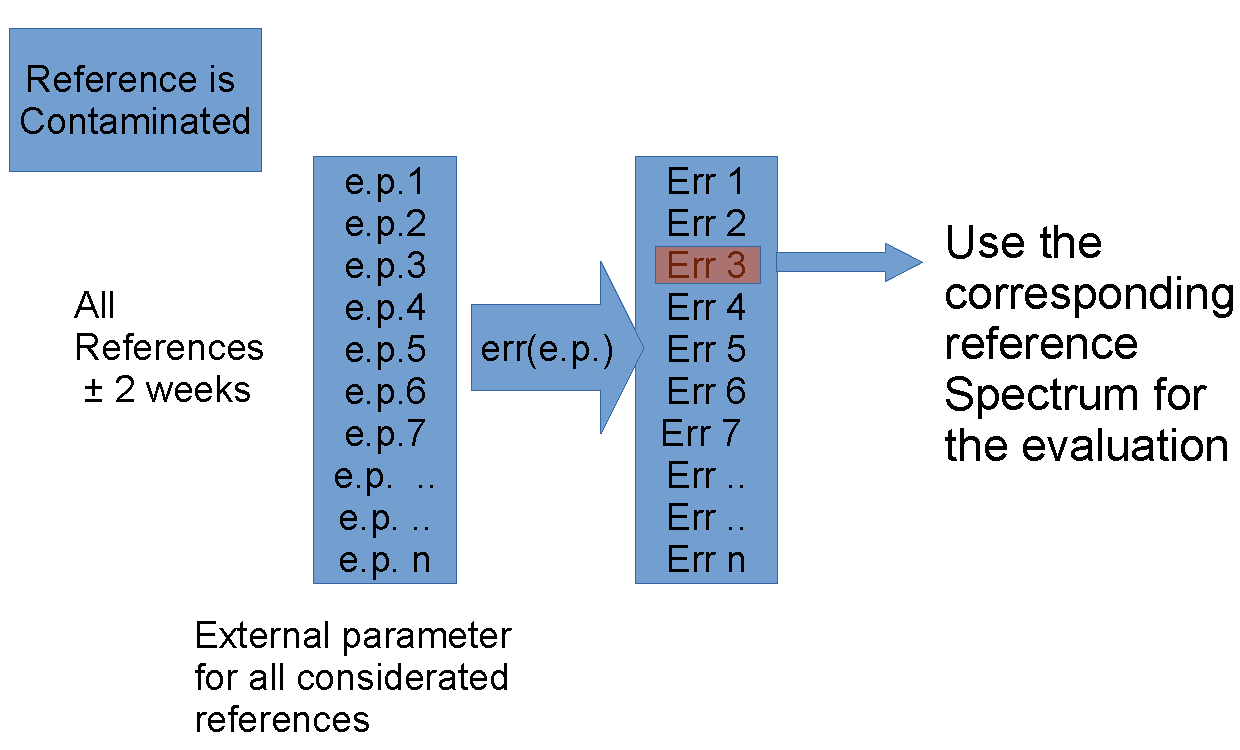
\includegraphics[width=0.7\linewidth]{Bilder/Cont}
\caption{}
\label{fig:Cont}
\end{figure}

	\begin{itemize}
		\item We have a list of possible references where all references are not contaminated and the temporal distance to the plume date is no longer than 14 days.
		\item we calculate of all possible references the differences in the external parameters
		\item We use the analysis of external parameters described above to estimate the \ce{BrO} error of all references
		\item We choose the reference with the smallest estimated \ce{BrO} error as new reference
		\item We evaluate the plume spectra with the new reference.
	\end{itemize}

	%
	The assumption is, that the \ce{BrO} error $\epsilon_{BrO}$ can be described as the sum of $\epsilon_{0}$ and the deviation of $\epsilon_{BrO}$ with respect to all external parameters. $\epsilon_{0}$ is the \ce{BrO} error when evalute the plume spectrum with the "same-time-reference", it is determined due to the accurateness of the NOVAC-instruments.
	\begin{align}
		\epsilon_{BrO} &=  \epsilon_{0}+\frac{d\epsilon}{dt}+\frac{d\epsilon}{d ^{\circ}}+\frac{d\epsilon}{dT}+\frac{d\epsilon}{ddt} +\frac{d\epsilon}{dc} + \mathcal{O}\left(OE\right) \\
		\rightarrow \Delta \epsilon_{BrO} &= \epsilon_{BrO} - \epsilon_{0} =\frac{d\epsilon}{dt}+\frac{d\epsilon}{d ^{\circ}}+\frac{d\epsilon}{dT}+\frac{d\epsilon}{ddt} +\frac{d\epsilon}{dc} + \mathcal{O}\left(OP\right) 
		\label{calc:err}
	\end{align}
	With $\epsilon_{BrO}$ describes the \ce{BrO} Error, t: time between plumetime and referencetime, T, temperaure; dt: daytime, c: colorindex, OP: other excluded external parameters\\
	The task occurring at this stage is to find the best representation for the deviations. An then find the reference which minimize $\Delta \epsilon_{BrO} $\\
	%
	\\
	%
	The easiest way is to just calculate the \ce{BrO} error of all possible references for every plume. Using this method we would be able to just choose the reference where the \ce{BrO} error is minimal. But this takes to much time since the evaluation would be proportional to the number of possible references because the evaluation need to be done for every plume-reference pair. Doing the evaluation for every plume-reference pair would make it impossible to do the evaluation in real, or near real time.\\
	%
	But we use this optimal evaluation to rate our model and compare them among each other. The optimal evaluation always choose the reference with the smallest absolute error. We don't use the relative error due to his vulnerability. Using the relative error could lead to a less preciseness.\\
	%
	\\
	Hier ein Bild, das eine Plume gegen viele referencen auswertet und hier die Abweichungen zeigt\\
	\\
	%
	The results of the algorithm which chooses the reference automatically are described relative to an optimal evaluation. If the relative error is larger than 5 we don't use the data.\\
	\\
	We tried several methods for choosing the best reference based on the analysis of external parameters. Fitting the data with a first order polynomial brought the best results.
	
	
	\section{Fit data}
	When looking at the analysis of the external parameters (see fig. \ref{fig:difftemp}-\ref{fig:diffexptime}) we can observe curves which are symmetric to the zero position. Therefore we conclude that it makes no difference whether the difference of a specific external parameter is positiv or negativ. Thus we take the absolute values for our calculations.\\
	\\
	%
	If we assume that all differentiations are linear, than we can write \cref{calc:err}
	as:  
	
	\begin{equation}
		\Delta \epsilon_{BrO} = a_{t}\cdot\Delta t+a_{^{\circ}}\cdot\Delta ^{\circ}+a_{T}\cdot\Delta T+a_{dt}\cdot\Delta dt +a_{c}\cdot\Delta c + \mathcal{O}\left(OP\right)
		\label{calc:delterr}
	\end{equation}
	%
	We used the same data as in \cref{fig:difftemp}-\ref{fig:diffexptime} to get the coefficients $a_{x}$ of \cref{calc:delterr}. We used on ordinary least square linear regression to get the coefficients $a_{x}$. In particular we used the python function LinearRegression from the library sklearn \cite{SKlearn}.  
	
	In \cref{Chap:BROErr} the dependency of the BrO error on external parameters are discussed. The question occurring here is, which parameters should we use for the algorithm which choose the reference automatic?
	To answer this question for the fitting routine we evaluated data of Tungurahua and Nevado Del Ruiz with different combinations of the external parameter described in \cref{Chap:BROErr}. Since we could not observe any correlation between the BrO Error and the Elevation angle the external parameter elvation angle was neglected in this analysis. To rate the results for the single instruments (three at Tungurahua and two at Nevado Del Ruiz) the difference to the "optimal evaluation" (explained in \ref{optimal evaition}) was used. Hereby the factor x, a quantity which describes the distinction between the optimal-Method and the contamination based method serves as indicator:
	\begin{equation}
	X = \frac{1}{n}\sum_{k}^{n} \frac{EContBased_{ k}}{EOpt_{ k}}
	\end{equation}
	$n$ is the total amount of contaminated spectra, $EOpt$ is the BrO error, in the optimal-evaluation, $EContBased$ is the BrO error, in the contamination based-evaluation. 
	\Cref{fig:WelcheEP} shows the calculations of the x factor for th e Tungurahua and the Nevado Del Ruiz volcano. The x-axis shows the external parameter used for the factor X. The y-axis shows the added factors x for every instrument at the volcanoes. The x factors were weighted with the percentage amount of data. We can see, that for both volcanoes the x factor is minimal for the combination of the following external parameters:\\
	\textit{$\bullet$ Temperature  $\bullet$ Daytime  $\bullet$ Exposure Time  $\bullet$ Temporal Difference}
	The factors X change from instrument to instrument. The results for every instrument can be seen in the appendix (\cref{fig:I2J8548}). The factors X range from xxxxxxx to xxxxxxxxxxxx.
	\begin{figure}
		\subfigure[Nevado Del Ruiz]{
		\includegraphics[width=0.5\linewidth]{"Bilder/WelcheEP/Nevado Del Ruiz"}}
		\subfigure[Tungurahua]{
		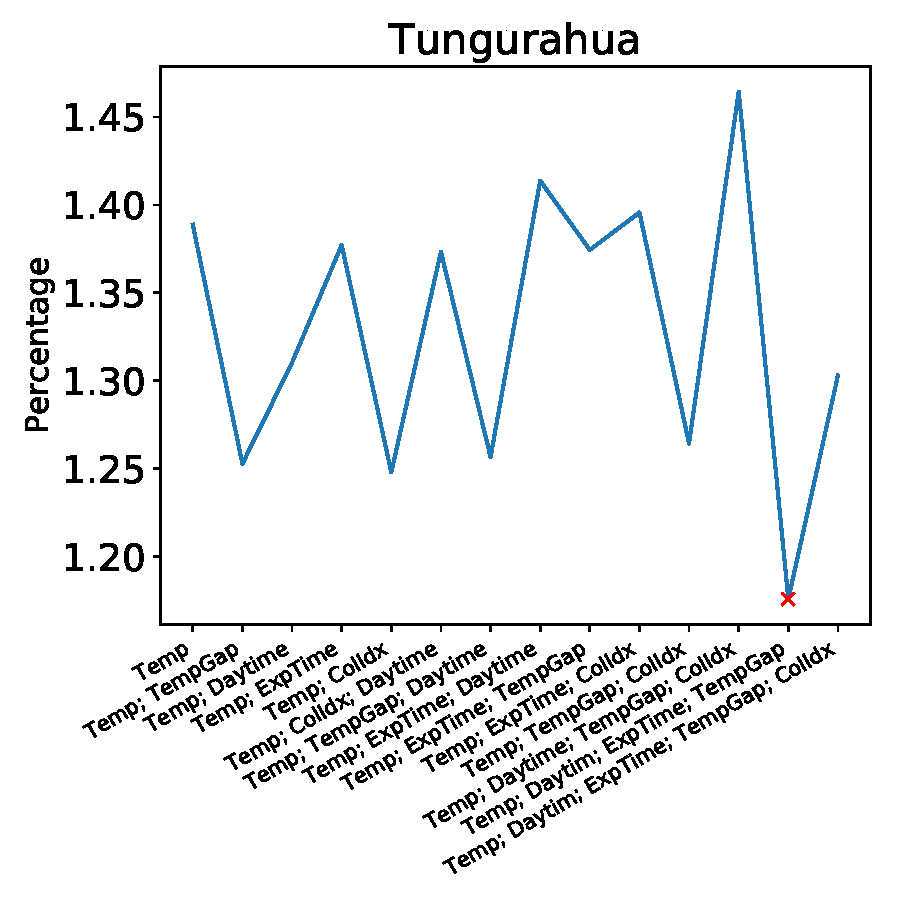
\includegraphics[width=0.5\linewidth]{Bilder/WelcheEP/Tungurahua}}
		\caption{}
		\label{fig:WelcheEP}
	\end{figure}

	

	

		
		The constants for Tungurahua and Nevado Del Ruiz are:
		\begin{table}
			\subfigure[Data of Nevado Del Riz D2J2201\_0]{
			\begin{tabular}{c|c|c}
				\toprule
				Constant &value & importance\\
				\toprule
				$a_{T}$&  7.338e+12&0.840\\
				\midrule
				$a_{ET}$&1.545e+10&0.045\\
				\midrule
				$a_{t}$&-2.6e+09& 0.0\\
				\midrule
				$a_{dt}$&1.805e+12&0.091\\
				\midrule
				$a_{c}$&2.301e+13& 0.031\\
				\bottomrule
			\end{tabular}}
			%	\caption{Data from Nevado Del Ruiz from the D2J2201\_0 instrument. All external parameter where taken into account. $\epsilon_{0} = =  5.404e+12$}
			\qquad
			\subfigure[Data of Nevado Del Riz D2J2200\_0]{
			\begin{tabular}{c|c|c}
				\toprule
				Constant &value & importance \\
				\toprule
				$a_{T}$& 1.162e+13&0.908 \\
				\midrule
				$a_{ET}$&2.811e+10& 0.046\\
				\midrule
				$a_{t}$&-1.7e+09& 0.0\\
				\midrule
				$a_{dt}$&1.076e+12&0.034\\
				\midrule
				$a_{c}$& 3.587e+13& 0.016\\
				\bottomrule
			\end{tabular}}
					\subfigure[Data of Nevado Del Both Instruments]{
			\begin{tabular}{c|c|c}
				\toprule
				Constant &value & importance \\
				\toprule
				$a_{T}$& 1.073e+13&0.973 \\
				\midrule
				$a_{ET}$&3.478e+10&  0.070\\
				\midrule
				$a_{t}$&-9.1e+08& 0.0\\
				\midrule
				$a_{dt}$& 1.523e+11&0.006\\
				\midrule
				$a_{c}$& -6.811e+13& -0.047\\
				\bottomrule
		\end{tabular}}
			\caption{(a)Data from Nevado Del Ruiz from the D2J2201\_0 instrument. All external parameter where taken into account. $\epsilon_{0} = =  5.404e+12$
				(b)Data from Nevado Del Ruiz from the D2J2200\_0 instrument. All external parameter where taken into account. $\epsilon_{0} = =  1.105e+13$ (c) Data from Nevado Del Ruiz from both instrument. All external parameter where taken into account. $\epsilon_{0} = 1.260e+13$}
		\label{tab:coef}
		\end{table}	


	\begin{itemize}
	
		\item Plume data are reliable if the \ce{SO2} column density is larger as 7 $\cdot 10^{17} \frac{molec}{cm^2}$
		\item Data are above the detection limit if the column density as two times larger than the fit error.
		\item If the reference is contaminated:

	\end{itemize}
	\begin{figure}
		\centering
%		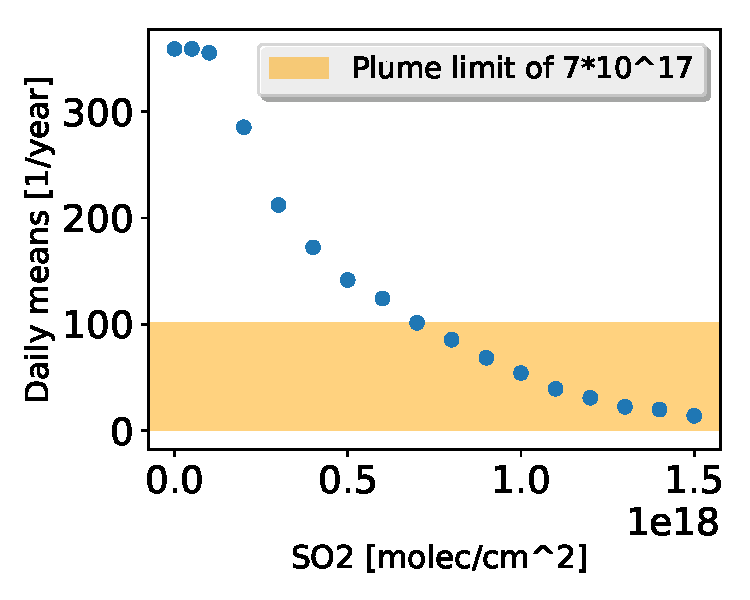
\includegraphics[width=0.7\linewidth]{E:/Masterarbeit/Analyse_minSO2/percentage_minSO2}
		\caption{}
		\label{fig:percentageminso2}
	\end{figure}
	\begin{figure}
		\centering
%		\includegraphics[width=0.7\linewidth]{E:/Masterarbeit/Analyse_minSO2/data_minSO2}
		\caption{}
		\label{fig:dataminso2}
	\end{figure}
			\begin{table}[h]
		%		\begin{tabular}{|p{2cm}|p{2.5cm}|p{1.5cm}|p{1.5cm}||p{1cm}|}
		%		%	\toprule
		%			&& Error & Amount of Data&davon gültig\\
		%			\toprule
		%			\multirow{2}{5em}{All Variables} 
		%				& independent& 1.51 & 95$\%$&10,5$\%$\\
		%				& dependent & 1.40&176 &14\\
		%			\midrule
		%			\multirow{2}{5em}{Exposure Time}
		%					&  independent &1.47&174&18\\
		%					& All &1.39&176&13\\
		%			\midrule
		%			\multirow{2}{5em}{Exp.Time u Coloridx}
		%					&  independent &1.4&175&20\\
		%					& All &1.35&176&13\\
		%			\bottomrule
		%		\end{tabular}
		\begin{tabular}{|p{2cm}|p{2.5cm}|p{1.5cm}|p{1.5cm}||p{1cm}|}
			%	\toprule
			&& Error & Amount of Data&valid data\\
			\toprule
			\multirow{2}{5em}{All Variables} 
			& independent& 1.51 & 95$\%$&10,5$\%$\\
			& dependent & 1.40&98$\%$ &8$\%$\\
			\midrule
			\multirow{2}{5em}{Exposure Time}
			&  independent &1.47&97$\%$&10$\%$\\
			& All &1.39&98$\%$&7$\%$\\
			\midrule
			\multirow{2}{5em}{Exp.Time u Coloridx}
			&  independent &1.40& 98$\%$&11\\
			& All & 1.35& 98$\%$&7$\%$\\
			\bottomrule
		\end{tabular}
	\end{table}


	\begin{table}[h]
		\centering
		{Evaluation of all contaminated data from Nevado Del Ruiz}
		\vspace*{1cm}
		\begin{tabular}{|p{2.2cm}|p{4.4cm}|p{5.0cm}|}
			\toprule
			Instrument& Dev from opt eval. (mean/median) & valid data\\
			\toprule
			$D2J2201\_0$ &1.14 / 0.82293& 128/283 = 45.2\%\\
			\midrule
			$D2J2200\_0$ &1.5 / 0.89965&954/1109 = 86.0\%\\
			\midrule 
			Both &1.26/0.847&1073/1392 = 77.1\%\\
			\bottomrule
		\end{tabular}
	\caption{Data from Nevado Del Ruiz from the D2J2201\_0 instrument. All external parameter where taken into account. $\epsilon_{0} = =  5.404e+12$}
	\end{table}
	\section{Other approaches}

	$\bullet$ In the optimal results are 15$\%$ valid data
	\begin{itemize}
		\item We also tried other possibilities than fitting to find the reference where the \ce{BrO} error is minimal. In the following we present two additional possibilities but compared to fitting the results are not as good.
	\end{itemize}
	\subsection{Nearest neighbours}
	\begin{itemize}
		\item Description of the Nearest Neighbours Method
	\end{itemize}
		\textcolor{red}{Nearest neighbor search (NNS), as a form of proximity search, is the optimization problem of finding the point in a given set that is closest (or most similar) to a given point. Closeness is typically expressed in terms of a dissimilarity function: the less similar the objects, the larger the function values. Formally, the nearest-neighbor (NN) search problem is defined as follows: given a set S of points in a space M and a query point q$\in$ M, find the closest point in S to q. Donald Knuth in vol. 3 of The Art of Computer Programming (1973) called it the post-office problem, referring to an application of assigning to a residence the nearest post office. A direct generalization of this problem is a k-NN search, where we need to find the k closest points.	
		Most commonly M is a metric space and dissimilarity is expressed as a distance metric, which is symmetric and satisfies the triangle inequality. Even more common, M is taken to be the d-dimensional vector space where dissimilarity is measured using the Euclidean distance, Manhattan distance or other distance metric. However, the dissimilarity function can be arbitrary. One example are asymmetric Bregman divergences, for which the triangle inequality does not hold.}
	\subsection{Iterative}
	\begin{itemize}
		\item Description of the iterative Method
	\end{itemize}
	The idea of the iterative method was, that the importance of the individual external parameters are very different, that means if we have the list of possible references, we took all referenes where the temperature difference is minimal, so we get a new, much smaller list of possible referenecs. From this list we choose all references where the next external parameter for example the daytime is minimal and get again a new list. We proceed this way with the following external parameters. We experiment with the sequence of the parameters, to increase the success of the method. The final sequence was:
	\begin{equation*}
	Temperature \bullet ................
	\end{equation*} 
	
	\chapter{Comparison with NOVAC Evaluation}
	This chapter shows and discuss the difference of the BrO, SO2 and BrO/So2 ratio data when evaluating with the NOVAC-Method, or with the contamination based method.
	The aim is to discover the systematic differences between the different retrievals and to discuss the reliability of the data.\\
	The following external parameter where used for the evaluation:
	\begin{itemize}
		\item Temperature
		\item Daytime
		\item Colorindex
		\item check das noch mal
	\end{itemize}
	To obtain the reference with minimal expected  BrO error the calculation of \cref{calc:delterr} and the corresponding coefficients from \cref{tab:coef} were used. The maximal temporal difference between measuring the reference and the plume is two weeks.
	\Cref{fig:diffNovac} shows a comparison of the data when evaluating with the NOVAC-method and the contamination based method. The x axis shows the column density calculated with NOVAC-method, the y axis shows the column density calculated the the contamination based method. Only data are used where the corresponding SO2 column density lies above the plume limit ($SO2\_SCD>7\cdot 10^{17}$). Meaning the column densities evaluated with the contamination based method. The corresponding SO2 SCD's evaluated with NOVAC could be below $7\cdot 10^{17}$.
	The plots at the left side show the results from the Tungurahua volcano while the plots at the right side show the results from Nevado Del Ruiz volcano. The black solid line shows a linear fit of the data, the dotted line indicates where the both evaluation are equivalent. The BrO data are visualized in the plots at the top of \cref{fig:diffNovac}. \\
	\\
	Beschreibung\\
	\\
	In the middle of \cref{fig:diffNovac} are the results of SO2 visualized:\\
	\\
	Beschreibung\\
	\\
	The BrO/SO2 ratio is visualized at the bottom of \cref{fig:diffNovac}:\\
	\\
	Beschreibung\\
	\\
	Another interesting question is, whether the change in the gas column density respectively the ratio depends on the amount evaluated with the NOVAC-method. To check this dependency \cref{fig:diffcontbase} was plotted. The data used for this figure are the same as for \cref{fig:diffNovac}. 
	

	\begin{itemize}
		\item Results only for contaminated data
		\begin{itemize}
			\item Difference in \ce{SO2} data evaluated with NOVAC-method and contamination-based evaluation
			\item Difference in \ce{BrO} data evaluated with NOVAC-method and contamination-based evaluation
			\item Difference in \ce{BrO}/\ce{SO2} Ratio data evaluated with NOVAC-method and contamination-based evaluation
		\end{itemize}
		\item Amount of \ce{BrO} data more than before (valid and not valid and above dection limit)
		\item Amount of \ce{SO2} data more than before (valid and not valid and above dection limit)
		\item Amount of \ce{BrO}/\ce{SO2} data more than before (valid and not valid and above dection limit)
		\item More \ce{BrO} data: 51\%
		\item  More valid \ce{BrO} data: 38\%
		\item Compare the dayly means: how many more data? due to higher S02 values
		\item 
	\end{itemize}
	
	\begin{figure}[h]		
		\subfigure[Data of Tungurahua]{\includegraphics[width=0.49\textwidth]{Bilder/Tungurahua_Pic/tung_bro_novac_conbased}}
		\subfigure[Data of Nevado Del Riz]{\includegraphics[width=0.49\textwidth]{Bilder/NevadoDelRuiz_Pic/bro_novac_conbased}}
		\subfigure[Data of Tungurahua]{\includegraphics[width=0.49\textwidth]{Bilder/Tungurahua_Pic/tung_so2_novac_conbased}}
		\subfigure[Data of Nevado Del Riz]{\includegraphics[width=0.49\textwidth]{Bilder/NevadoDelRuiz_Pic/so2_novac_conbased}}
%		\subfigure[Data of Tungurahua]{\includegraphics[width=0.49\textwidth]{Bilder/Tungurahua_Pic/tung_ratio_novac_conbased}}
%		\subfigure[Data of Nevado Del Riz]{\includegraphics[width=0.49\textwidth]{Bilder/NevadoDelRuiz_Pic/ratio_novac_conbased}}
		\caption{The dependency of the Difference between contamination based data and NOVAC to the data evaluated with the NOVAC data }
		\label{fig:diffNovac}
	\end{figure}
		\begin{figure}[h]		
			\subfigure{\includegraphics[width=0.49\textwidth]{Bilder/Tungurahua_Pic/tung_ratio_novac_conbased}}
			\subfigure{\includegraphics[width=0.49\textwidth]{Bilder/NevadoDelRuiz_Pic/ratio_novac_conbased}}
			\subfigure{\includegraphics[width=0.49\textwidth]{Bilder/Tungurahua_Pic/tung_ratio_diff_novac_conbased}}
			\subfigure{\includegraphics[width=0.49\textwidth]{Bilder/NevadoDelRuiz_Pic/ratio_diff_novac_conbased}}
		\end{figure}
	%
\begin{figure}
	\centering
	\includegraphics[width=0.7\linewidth]{Bilder/BarPlot}
	\caption{}
	\label{fig:barplot}
\end{figure}

	\chapter{Results}
	Interpretation of the \ce{BrO}/\ce{SO2} ratio time-series
	\section{Tungurahua}
	\begin{figure}
		\centering
		\includegraphics[width=0.7\linewidth]{Bilder/Results/Results_Tungurahua}
		\caption{}
		\label{fig:resultstungurahua}
	\end{figure}
	
	\begin{small}	
	\begin{align*}
	&Menge an Daten insgesamt: &5883 &\equiv &1\\
	&\hspace*{1cm} Davon: (NOVAC Auswertung) über plume limit&712 &\equiv & 0.121\\
	&\hspace*{1cm}Davon: Menge an Daten, die nicht Kontaminiert sind: &5504 &\equiv & 0.936\\
	&\hspace*{2cm}Davon im Plume-limit:  &599   &\equiv & 0.102\\
	&\hspace*{2cm}Davon über dem Detection Limit:&36  &\equiv & 0.006\\
	&\hspace*{1cm}Davon sind kontaminiert:  &379  &\equiv & 0.064\\
	&\hspace*{2cm}Davon (mit NOVac ausgewertet) über plume limit: &114  &\equiv &0.301 \\
	&\hspace*{2cm}Davon (Neue Auswertung) über plume limit &185  &\equiv &0.488\\
	\end{align*}	
	Dh in den kontaminierten daten sind mit NOVAC ausgewerteten daten \underline{2.485} häufiger über dem plume limit\\	

	\end{small}
	\section{Nevado Del Ruiz}
		\begin{figure}
		\centering
		\includegraphics[width=0.7\linewidth]{"Bilder/Results/Results_NevadoDelRuiz (1)"}
		\caption{}
		\label{fig:resultsnevadodelruiz-1}
	\end{figure}
	\begin{small}	
	\begin{align*}
		&Menge an Daten insgesamt:  &8962 &\equiv &1\\
		&\hspace*{1cm} Davon: (NOVAC Auswertung) über plume limit&142  &\equiv &0.016\\
		&\hspace*{1cm} Davon: nicht kontaminierte daten: &8596 &\equiv &0.959\\
		&\hspace*{2cm} Davon im Plume-limit:   &123  &\equiv &0.014\\
		&\hspace*{2cm} Davon über dem Detection Limit: &53   &\equiv &0.006\\
		&\hspace*{1cm} Davon sind kontaminiert:  &366  &\equiv &0.041\\
		&\hspace*{2cm} Davon (mit NOVac ausgewertet) über plume limit: &20   &\equiv &0.055\\
		&\hspace*{2cm} Davon  (Neue Auswertung) über plume limit&179 &\equiv &0.489\\
		\end{align*}
	Dh in den kontaminierten daten sind mit NOVAC ausgewerteten daten \underline{3.449} häufiger über dem plume limit\\
 	
 \end{small}
	\chapter{Issues of our method}
	
	\section{Contamination of the plume}
	\begin{itemize}
		\item As discussed above it might occur, that, that the reference is contaminated for example by the plume of the day before. If that happens, we underestimate the gas amount by using a contaminated reference. But another possibility is, that the plume is also contaminated. This might be the case if the volcanic gas of the volcano is not taken away by the wind, but accumulates in the plume. If this is the case, using an other reference would lead to an overestimation of the column density of gases.
	\end{itemize}

	\chapter{Conclusion}
	....
	
	
	



  \part{Appendix}
  \begin{appendix}
	\begin{figure}
		\subfigure[]{\includegraphics[width=0.45\linewidth]{Bilder/WelcheEP/D2J2140}}
		\subfigure[]{\includegraphics[width=0.45\linewidth]{Bilder/WelcheEP/D2J2200_0}}
		\subfigure[]{\includegraphics[width=0.45\linewidth]{Bilder/WelcheEP/D2J2200_1}}
		\subfigure[]{\includegraphics[width=0.45\linewidth]{Bilder/WelcheEP/D2J2201_0}}
		\subfigure[]{\includegraphics[width=0.45\linewidth]{Bilder/WelcheEP/I2J8546}}
		\subfigure[]{\includegraphics[width=0.45\linewidth]{Bilder/WelcheEP/I2J8548}}
		\caption{}
		\label{fig:I2J8548}
		\end{figure}

    \chapter{Lists}
    \listoffigures
    \listoftables
    \bibliography{references}{}
    \citestyle{egu}
    \bibliographystyle{plainnat}
    \setlength{\parindent}{0em}

Erkl\"{a}rung:\par
\vspace{3\baselineskip}
Ich versichere, dass ich diese Arbeit selbstst\"{a}ndig verfasst habe und keine
anderen als die angegebenen Quellen und Hilfsmittel benutzt habe.\par
\vspace{5\baselineskip}
Heidelberg, den (Datum)\hspace{3cm}\dotfill

  \end{appendix}
\end{document}




